%\documentclass[draftdoc]{JSBMLdoc}
\documentclass{JSBMLdoc}
\usepackage{dirtree}
\usepackage{makeidx}
\usepackage[font=small,totoc]{idxlayout}

\makeindex

%%%%%%%%%%%%%%%%%%%%%%%%%%%%%%%%%%%%%%%%%%%%%%%%%%%%%%%%%%%%%%%%%%%%%
% 
% A collection of useful macros that facilitat maintaining the JSBML
% documentation.
%
% Author: Andreas Dr\"ager
%%%%%%%%%%%%%%%%%%%%%%%%%%%%%%%%%%%%%%%%%%%%%%%%%%%%%%%%%%%%%%%%%%%%%

% A
\newcommand{\AbstractNamedSBase}{\texttt{AbstractNamedSBase}\index{SBase@\texttt{SBase}!\texttt{AbstractNamedSBase}}}
\newcommand{\ASTtype}{\texttt{AST\_TYPE\_*}\index{ASTNode@\texttt{ASTNode}!\texttt{AST\_TYPE\_*}}}
\newcommand{\ASTNode}{\texttt{ASTNode}\index{ASTNode@\texttt{ASTNode}}}

% C
\newcommand{\CallableSBase}{\texttt{CallableSBase}\index{JSBML!CallableSBase@\texttt{CallableSBase}}\index{SBase@\texttt{SBase}!CallableSBase@\texttt{CallableSBase}}}
\newcommand{\Compartment}{\texttt{Compartment}\index{SBML!Compartment@\texttt{Compartment}}}

% H
\newcommand{\History}{\texttt{History}\index{annotation!\texttt{History}}}

% K
\newcommand{\KineticLaw}{\texttt{KineticLaw}\index{KineticLaw@\texttt{KineticLaw}}}

% M
\newcommand{\Model}{\texttt{Model}\index{model!Model@\texttt{Model}}}
\newcommand{\ModelCreator}{\texttt{ModelCreator}\index{annotation!\texttt{ModelCreator}}}
\newcommand{\ModelHistory}{\texttt{ModelHistory}\index{annotation!\texttt{ModelHistory}}}

% N
\newcommand{\NamedSBase}{\texttt{NamedSBase}\index{SBase@\texttt{SBase}!\texttt{NamedSBase}}}

% S
\newcommand{\SBase}{\texttt{SBase}\index{SBase@\texttt{SBase}}}
\newcommand{\SBML}{SBML\index{SBML}}
\newcommand{\SBMLDocument}{\texttt{SBMLDocument}\index{SBML!SBMLDocument@\texttt{SBMLDocument}}}
\newcommand{\Serializable}{\texttt{Serializable}\index{Serializable@\texttt{Serializable}}}
\newcommand{\Species}{\texttt{Species}\index{SBML!Species@\texttt{Species}}}

% T
\newcommand{\TreeNode}{\texttt{TreeNode}\index{TreeNode@\texttt{TreeNode}}} 

% U
\newcommand{\UnitDefinition}{\texttt{UnitDefinition}\index{Unit!UnitDefinition@\texttt{UnitDefinition}}}

\hyphenation{
AST-Node
Boo-lean
Cell-De-sig-n-er
Call-able-S-Base
Event-Listener
Event-Hand-l-er
Event-Object
get-Ex-po-nent
get-Ex-po-nent-As-Double
get-Spatial-Di-men-sions
get-Spatial-Di-men-sions-As-Double
J-SB-ML
Ki-ne-tic-Law
lib-SBML-Constants
Lib-SB-ML-Reader
Local-Pa-ra-meter
Plug-in-Action
plug-in
Property-Change-Event
SBML-Document
Tree-Node
Tree-Node-Change-Event
Tree-Node-Change-Listen-er
Tree-Node-With-Change-Support
time-Units
Tree-Node
}


\hypersetup{
  bookmarksopenlevel={1},
  bookmarksnumbered={true},
  breaklinks={true},
  pdfpagemode={UseOutlines},
  pdftitle={User guide for JSBML},
  pdfauthor={Andreas Dr\"ager} {Nicolas Rodriguez} {Alex Thomas} {Marine Dumousseau}
 {Alexander D\"orr} {Clemens Wrzodek} {Finja B\"uchel}
{Florian Mittag} {Nicolas Le Nov{\`e}re} {Andreas Zell} {Michael Hucka},
  pdfsubject={Software guide},
  pdfkeywords={JSBML} {libSBML} {Java} {SBML} {API} {LaTeX} {documentation}
{manual} {guide} {code examples},
  pdfview={FitV},
  pdffitwindow={true},
  pdfstartview={FitV},
  pdfnewwindow={false},
  pdfdisplaydoctitle={true},
  pdfhighlight={/P},
  plainpages={false},
  unicode={true}
}

% -----------------------------------------------------------------------------
\begin{document}

\title{\textls[20]{User Guide for JSBML}}

\version{1.0 \\[0.5em]{\normalsize Document version: 24 October 2014}}

\newcommand{\where}[1]{\,\textsuperscript{#1}}
\newcommand{\divider}[1]{\multicolumn{3}{c}{\emph{#1}:}}

\author{%
  \setlength{\tabcolsep}{20pt}%
  \begin{tabular}{@{}ccc@{}}
    \divider{Authors}\\[0.75em]
    Andreas Dr\"ager\where{a,b}   & Nicolas Rodriguez\where{c,d} & Alex Thomas\where{a}\\
    Marine Dumousseau\where{d}    & Alexander D\"orr\where{b}    & Clemens Wrzodek\where{b}\\
    Finja B\"uchel\where{b}       & Florian Mittag\where{b}      & Michael Hucka\where{e}\\[2em]
    \divider{Principal investigators}\\[0.75em]
    Bernhard \O. Palsson\where{a} & Andreas Zell\where{b}        & Nicolas Le Nov\`ere\where{c,d}\\
                                  & Michael Hucka\where{e}\\[2em]
    \divider{Institutional affiliations}\\[0.5em]
  \end{tabular}
  \\
  \begin{normalsize}
  \where{a\,}Systems Biology Research Group, University of California, San Diego, La Jolla, CA, USA
  \\[0.25em]
  \where{b\,}Center for Bioinformatics Tuebingen, University of Tuebingen, T\"ubingen, Germany
  \\[0.25em]
  \where{c\,}The Babraham Institute, Babraham Campus, Cambridge, UK
  \\[0.25em]
  \where{d\,}European Bioinformatics Institute, Wellcome Trust Genome Campus, Hinxton, Cambridge, UK
  \\[0.25em]
  \where{c\,}Computing and Mathematical Sciences, California Institute of Technology, Pasadena, CA, USA
  \end{normalsize}
}

\frontNotice{SBML (the Systems Biology Markup Language) is an XML-based
  format for storing and exchanging computational descriptions of
  biological processes.  To read, write, manipulate, and perform
  higher-level operations on SBML files and data streams, software
  applications need to map SBML entities to suitable software objects.
  JSBML provides a pure Java library for this purpose.  It supports all
  Levels and Versions of SBML, and provides many powerful features,
  including facilities to help migrate from the use of libSBML (a popular
  library for SBML that is not written in Java).
  \\ \\
  This document provides an introduction to JSBML and its use.  It is aimed
  at both developers writing new Java-based applications as well as those
  who want to adapt libSBML-based applications to using JSBML.  This user
  guide is a companion to the JSBML API documentation.
  \\ \\
  \centerline{The JSBML home page is \url{http://sbml.org/Software/JSBML/}.}\\
  \centerline{The JSBML discussion group is \url{http://sbml.org/forums/jsbml-development}.}
}


\maketitlepage
\maketableofcontents
\clearpage


\chapter{Getting started with JSBML}
\label{chp:getting-started}

JSBML is a Java\TTra library that will help you to read, write and
manipulate SBML files~\cite{Draeger2011a, Draeger2011b}. This chapter
provides information for quickly getting started with using JSBML.

Before you can use JSBML, you will need to obtain a copy of the library.
\sec{sec:obtaining-jsbml} below describes different ways of doing
this, and explains which additional libraries you may need. JSBML also
requires the use of a Java Runtime Environment (JRE) version~1.5 or
later~\cite{JavaDownloadURL}. \index{Java Runtime Environment (JRE)} In the
rest of this document, we assume that you have already installed a suitable
JRE or Java Development Kit (JDK), and know how to configure the Java class
path on your system. \index{Java Development Kit (JDK)}

It is also essential to \emph{understand SBML} in order to be able to use
it (and JSBML) properly. If you are not already familiar with SBML, a good
starting point for learning about it is the latest SBML
specification~\cite{SBMLspecs}. You can find answers to many questions in
the SBML FAQ~\cite{SBMLFAQ} and optionally by asking on one of the SBML
discussion lists~\cite{SBMLforums}.

% -*- TeX-master: "User_guide"; fill-column: 75 -*-

\section{Obtaining and using JSBML}
\label{sec:obtaining-jsbml}

We provide four options for obtaining a copy of JSBML: (1) download the JAR
file distribution for JSBML complete with dependencies, that is, packaged
with third-party Java libraries needed by JSBML; (2) download the JAR file
distribution for JSBML \emph{excluding} dependencies; (3) download the
source code distribution; and (4) obtain the source code directly from the
project's Subversion repository. These four options are described below.


\subsection{The JSBML archive with dependencies}

The version of the archive that includes dependencies is a merged JAR file
that contains all of JSBML's required third-party libraries. You can
download it from the JSBML area on SourceForge~\cite{JSBMLdownload}. Once
you have installed the JAR file on your computer, it is sufficient to add
it to your Java build and/or class path in order to use JSBML.

\subsection{The JSBML archive without dependencies}

\begin{table}[b]
  \caption{List of other, third-party libraries needed by JSBML.}
  \label{tab:dependencies}
  \centering
  \rowcolors{2}{sbmlrowgray}{}
  \renewcommand{\arraystretch}{1.1}
  \begin{tabular}{>{\ttfamily}lp{2.26in}l}
    \toprule
    \textbf{\sffamily Library name} & \textbf{Purpose} & \textbf{Source URL} \\
    \midrule
    biojava-ontology-4.0.0.jar
    & biojava ontology-related classes~\citep{Holland2008}.
    \index{Ontology}
    & \href{http://biojava.org}{biojava.org} \\

    junit-4.8.jar
    & Unit-test support library; only needed if you \mbox{intend} to
    run the tests in the \code{tests} folder.
    & \href{http://www.junit.org}{www.junit.org} \\

    stax2-api-3.1.4.jar
    & Used for reading and writing XML.
    & \href{http://docs.codehaus.org/display/WSTX/StAX2}{docs.codehaus.org/display/WSTX/StAX2} \\

    woodstox-core-5.0.1.jar
    & Used for reading and writing XML.
    & \href{http://woodstox.codehaus.org}{woodstox.codehaus.org} \\
    
    staxmate-2.3.0.jar
    & Used for reading and writing XML. Provides a more user-friendly StAX
    interface.
    & \href{http://staxmate.codehaus.org}{staxmate.codehaus.org} \\

    xstream-1.3.1.jar
    & Used for reading and writing XML, specifically parsing results from
    the SBML validator.
    & \href{http://xstream.codehaus.org}{xstream.codehaus.org} \\

    jigsaw-dateParser.jar
    & Portion of the \emph{Jigsaw} library (version from
    Dec. 2010), containing classes for date manipulation. 
    & \href{http://jigsaw.w3.org}{jigsaw.w3.org} \\

    log4j-1.2-api-2.3.jar 
    & Libraries for logging errors and other diagnostics.
    & \href{http://logging.apache.org/log4j}{logging.apache.org/log4j} and \href{http://www.slf4j.org}{slf4j.org} \\

    log4j-api-2.3.jar \\ log4j-core-2.3.jar \\ log4j-slf4j-impl-2.3.jar \\ slf4j-api-1.7.21.jar \\

    \bottomrule
  \end{tabular}
\end{table}

The version of the JSBML archive that excludes dependencies is a JAR file
that contains only JSBML classes. You can download it from the JSBML area
on SourceForge~\cite{JSBMLdownload}. Since it does not include the
third-party libraries needed by JSBML to operate, you will need to obtain
and download those libraries separately. \tab{tab:dependencies} lists
what they are. Once you have installed the JSBML JAR file \emph{and} these
third-party libraries on your computer, you will need to add them
\emph{all} to your Java build and/or class path in order to use JSBML.


\subsection{Maven dependencies}

JSBML can also be obtained through Apache Maven~\citep{ApacheMaven}.
If you are already using Maven in your project, you can add JSBML
as a dependency, just add the following lines into your pom.xml:

\begin{example}[language=XML, title={Maven instructions to add to your pom.xml.}]
  <repositories>
    <repository>
      <id>ebi-repo</id>
      <name>The EBI repository</name>
      <url>http://www.ebi.ac.uk/~maven/m2repo</url>
      <releases><enabled>true</enabled></releases>
    </repository>
  </repositories>

  <dependencies>
    <dependency>
      <groupId>org.sbml.jsbml</groupId>
      <artifactId>jsbml</artifactId>
      <version>|\jsbmlversion|</version>
    </dependency>
  </dependencies> 
\end{example}

The jsbml artifact will include jsbml-core plus all L3 packages. Like this
there is not need to list all the packages by hand and when
a new one is developed, you will get it without having to make too much change to your
pom files. 

If you want to pick which package to include, you can list them one by one, there are
further instructions at \url{http://sbml.org/Software/JSBML/docs/Maven_Configuration}.


\subsection{The JSBML source archive}
\label{sec:jsbml-source-archive}

The source distribution for JSBML is similar to the JAR distribution that
excludes third-party dependency libraries, except that the JSBML files are
not compiled into class files; you must compile them yourself. As with the
other options described above, the source distribution is available from
the JSBML area on SourceForge~\cite{JSBMLdownload}, as an archive file in
ZIP format.

Download whichever format is more convenient for you and unpack the archive
on your computer somewhere.  The act of unpacking the archive will create a
folder on your computer named after the distribution version; for
example, this may be ``\code{jsbml-}\jsbmlversion''.  Next, you will need to compile
the Java source code.  JSBML comes with a \emph{build file} (i.e., scripted
instructions in a specialized format) for Apache Ant~\citep{ApacheAnt};
you can use other approaches for compiling the JSBML classes and
performing other tasks, but Ant provides an especially convenient approach.
For the rest of the instructions below, we use Ant.  Here is an example of
how to compile the JSBML class files after you have unpacked the source
code archive:

\begin{example}[style=bash, title={Compiling JSBML with Ant; this example
    uses Bash shell syntax.}] 
cd jsbml-|\jsbmlversion|
ant compile
\end{example}

Next, if you wish to run the self-tests included with JSBML, you can do so by
running the following command:

\begin{example}[style=bash, title={Running the unit tests provided with JSBML.}]
ant test
\end{example}

Finally, if you want to produce a JAR file containing all the JSBML
compiled class files, run the following command:

\begin{example}[style=bash, title={Creating a JAR file.}]
ant jar
\end{example}



\subsection{The JSBML source code repository}
\label{sec:SourceDistribution}

The fourth approach to obtaining a copy of JSBML is to retrieve it directly
from the Subversion repository~\cite{JSBMLSVN}.  Here is an example of how
to retrieve the latest version of the JSBML sources:

\newcommand{\dirname}{\code{\emph{\color{winered}jsbml}}\xspace}

\begin{example}[style=bash, title={Downloading the latest JSBML 
    sources from the JSBML project's Subversion repository.}]
svn co https://svn.code.sf.net/p/jsbml/code/trunk |\dirname|
cd |\dirname|
\end{example}

(The name you give to the copy on your computer is up to you.  We used
``\dirname'' in this example, but you could name the folder something else
if you wish.)  Once you have retrieved the folder from the Subversion
repository, you can compile the source files and create a JAR file.  Please
refer to the instructions in \sec{sec:jsbml-source-archive}.

The Subversion repository contains copies of all the third-party libraries
listed in \tab{tab:dependencies} and needed by JSBML.  They are
located in the folder ``\dirname''\code{/core/lib}.


\subsection{Setting up Eclipse}
\label{sec:SettingUpEclipse}

To set up Eclipse to work with JSBML, first add the \texttt{src},
\texttt{test} and \texttt{resources} folder of the JSBML distribution to your
Eclipse build path, and add all of the \texttt{.jar} files found in the
\texttt{lib} folder.

Next, you need to do an extra step to configure the annotation processor,
because the different parsers in JSBML are registered automatically using
Java annotations.  To configure the annotation processor in Eclipse, follow
the instructions found on the web page
\url{https://github.com/niko-rodrigue/spi/blob/wiki/EclipseSettings.md}.
 The jar file of the annotation processor is located in the jsbml source tree at
 ``\dirname''\code{/core/lib/spi-full-0.2.4.jar}. If you checkout 
the full trunk (and not just the core), you can find a folder dev, which 
contains a README.txt file that has also these instructions and further 
important information.

Finally, you can run the \code{ParserManager} class to check that the list of
parsers are not empty and that they contain the parsers you need.


\subsection{Optional extensions, modules and examples available for JSBML}
\label{sec:dependencies}

JSBML provides a number of additional extensions, modules and example
programs that you may find useful in your work.  The \emph{extensions} are
optional add-ons that implement support for SBML Level~3 Packages; these
packages extend SBML syntax to support, for example, storing the layout of
a model's graphical diagram directly in the SBML file.  The JSBML
\emph{modules} provide additional features and interfaces, for example, to
allow CellDesigner~\cite{Funahashi2003} plugins to use JSBML.  Finally, the
JSBML \emph{examples} are full-fledged applications that demonstrate the
use of JSBML in actual running software.  Each of these optional components
of JSBML is available from the project's code repository (and in some
cases, from the download area on SourceForge~\cite{JSBMLdownload}).  In the
subsections below, we explain how to obtain copies of them from the
repository.


\subsubsection{JSBML Extensions}

The JSBML repository's \code{extensions} folder contains a separate
subfolder for each currently-implemented JSBML extension. You can either
retrieve a copy of each extension separately, or obtain the complete
\code{extensions} portion of the repository.  Here we explain the latter.

First, find a suitable location on your computer where you would like to
place the JSBML extensions folder.  (We suggest placing it side-by-side at
the same level as your JSBML core folder, e.g., next to the folder
``\dirname'' discussed above.)  Then, perform the following step:

\begin{example}[style=bash, title={Downloading the latest JSBML extensions
    source folder from the project's Subversion repository.}] 
svn co https://svn.code.sf.net/p/jsbml/code/trunk/extensions jsbml-extensions
\end{example}

Each of the extensions has its own Ant build script, located in a file
named (as per Ant conventions) ``\code{build.xml}'' within the extension's
subfolder.  To build, for example, the \code{layout} extension, you could
do the following:

\begin{example}[style=bash, title={Compiling the ``\code{layout}'' extension.}]
cd extensions/layout
ant compile
\end{example}


\subsubsection{JSBML Modules}
\label{sec:jsbml-modules}

JSBML currently provides six additional modules.  Each provides features
for task-specific purposes. Binary versions of the modules can be found at
the download site of JSBML~\cite{JSBMLdownload}; here we explain how you
can obtain the most recent versions of the modules directly from the source
code repository.  (Note: at the time of this writing, only the
\code{tidy}, \code{CellDesigner} and the \code{libSBMLio} module have been extensively
tested.)

First, find a suitable location on your computer where you would like to
place the JSBML modules folder.  We suggest creating a folder named
``\code{modules}'' placed side-by-side at the same level as your JSBML core
folder, e.g., next to the folder ``\dirname'' discussed above.

\begin{example}[style=bash, title={Creating a folder for the modules.}]
mkdir modules
cd modules
\end{example}

\newcommand{\modulename}{\code{\emph{\color{winered}modulename}}\xspace}

Next, perform the following operation, once for each of the modules you
would like to obtain, where the variable \modulename is one of the names
listed in the first column of \tab{tab:jsbml-modules}:

\begin{example}[style=bash, title={Obtaining a JSBML module.}]
svn co https://svn.code.sf.net/p/jsbml/code/trunk/modules/|\modulename| |\modulename|
\end{example}

(In other words, if you would like to obtain both the Android and libSBMLio
modules, execute the command above twice, once with \code{android} in place
of \modulename and a second time with \code{libSBMLio} in place of
\modulename.)  Once they're downloaded, please check inside each module
directory for information about how to use them.

\begin{table}[thb]
  \caption{JSBML modules available today.}
  \label{tab:jsbml-modules}
  \centering
  \rowcolors{2}{sbmlrowgray}{}
  \begin{tabular}{>{\ttfamily}lp{5.25in}}
    \toprule
    \textbf{\sffamily Module name} & \textbf{Purpose} \\
    \midrule
    android
    & Support for writing JSBML-based programs for Android OS.
    \\
    celldesigner
    & A bridge module that supports writing JSBML-based
    plugins for CellDesigner~\cite{Funahashi2003}
    \\
    compare
    & Facilities for doing comparisons between libSBML and JSBML
    \\
    libSBMLcompat
    & A module that allows easier switching between libSBML and JSBML by
    providing wrapper classes replicating much of libSBML's API in JSBML (in development)
    \\
    libSBMLio
    & A libSBML communications layer.
    \\
    tidy
    & A warper around the SBMLWriter class that use the jtidy library~\cite{jtidy} (a Java port of HTML Tidy) to
    format properly the resulting XML.
    \\
    \bottomrule
  \end{tabular}
\end{table}

You can find more information and explanation about JSBML's modules in \sec{sec:jsbml-modules-details}.


\subsubsection{JSBML Examples}
\label{sec:jsbml-repo-examples}

The JSBML repository's \code{examples} folder contains a separate
subfolder for each sample application.  To obtain them, first, find a
suitable location on your computer where you would like to place the JSBML
examples folder.  We suggest creating a folder named ``\code{examples}''
placed side-by-side at the same level as your JSBML core folder.

\begin{example}[style=bash, title={Creating a folder for the examples.}]
mkdir examples
cd examples
\end{example}

Next, retrieve the examples you would like to obtain.  At the time of this
writing, there is only one example available:

\begin{example}[style=bash, title={Retrieving the \emph{SBML Bar Graph}
    example application.}] 
svn co https://svn.code.sf.net/p/jsbml/code/trunk/examples/sbmlbargraph sbmlbargraph
\end{example}

Finally, please read the ``\code{README.txt}'' file in the freshly-obtained
\code{sbmlbargraph} folder to learn more about how to get started with the
example application.



% -*- TeX-master: "User_guide"; fill-column: 75 -*-

\section[Writing your first JSBML application]{\emph{Hello World}: writing your first JSBML applications}
\label{sec:hello-world}

In this section, we present two examples of using JSBML. The first is a
program that reads a file containing an SBML document and displays its
components in a Java \JTree graphical object. The second example
illustrates the creation of an object representing an SBML document (which,
in JSBML, is represented programmatically using an object of class
\SBMLDocument), as well as writing that object to a file. These basic
examples should help serve as a foundation for writing your own, more
elaborate programs.


\subsection{Reading and visualizing an \codeNC{SBMLDocument} object}

\fig{fig:JSBMLvisualizer-source} shows the listing of a simple program
called ``\code{JSBMLvisualizer}''.  The source is included in the JSBML
distribution, in the ``\texttt{doc/user\_guide/src}'' subdirectory.  As
with most simple JSBML-based programs, to compile and execute
``\code{JSBMLvisualizer}'', you would execute the following sequence of
commands:

\newcommand{\classpath}{\code{\emph{\color{winered}classpath}}\xspace}

\begin{example}[style=bash, title={Compiling and executing the example program.}]
  javac -classpath |\classpath|JSBMLvisualizer.java
  java -classpath |\classpath|JSBMLvisualizer
\end{example}

\begin{wrapfigure}[24]{r}{2.55in}
  \centering
  \vspace*{-1.8em}
  \setlength{\captionmargin}{1.8em}
  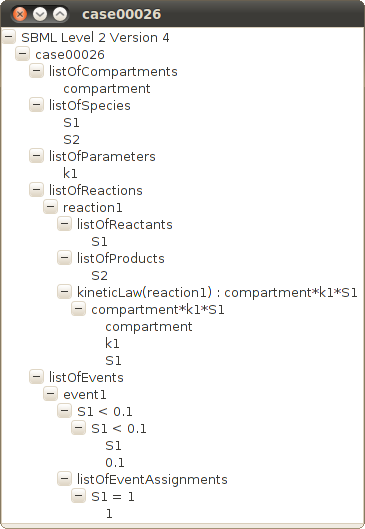
\includegraphics[width=.32\textwidth]{%
    ../posters/2010_ICSB_and_COMBINE/JSBMLvisualizerTransparent.png}
  \caption[Tree representation of an SBML file]{Tree representation of
    the contents of the SBML test file ``\code{case00026}.xml''. In JSBML,
    the hierarchically structured \SBMLDocument can be traversed
    recursively because all instances of \SBase, the parent class,
    implement the interface \TreeNode.}
  \label{fig:JSBMLvisualizer-output}
\end{wrapfigure}
In the example commands above, replace the placeholder text \classpath with
the actual Java class path for the JSBML libraries and its dependencies on
your particular computer; we do not show an exact value here because it
depends on where you have installed the JAR files for JSBML and the
third-party libraries.

When run, the program expects to be given the pathname of a valid SBML
file as \index{SBML!XML file} its sole argument. It uses the static method
\code{read()} defined by the JSBML object class \SBMLReader to read the
file; \SBMLReader returns an object of class \SBMLDocument, the main SBML
document container in JSBML.  Next, the program constructs a new
\code{JSBMLvisualizer} object, which is derived from the standard Java
\JFrame class. It invokes the class constructor (line 9) with the
identifier of the model in the SBML file, obtained by calling
\code{getModel().getId()} on the \SBMLDocument object; this sets the
\JFrame's title to the identifier of the model.  Since JSBML's \SBase
object (and all objects derived from it) implement the \TreeNode interface,
it is possible to create a \JTree directly from the information in an
\SBMLDocument object instance.  (To keep our examples short and focused on
the essentials of using JSBML, we have omitted error checking steps.  A
real application program should guard against various situations, such as
\code{getModel()} or \code{getId()} returning \code{null}, and take steps
to deal with them appropriately. You might also like to read SBML files in
a separate thread and monitor the progress of reading the file in some
progress bar.)

\begin{figure}[ht]
  \exampleFile[style=java, firstline=35, caption={}]{src/org/sbml/jsbml/gui/JSBMLvisualizer.java}
  \caption{Parsing and visualizing the content of an SBML file.}
  \vspace*{-1.5em}
  \label{fig:JSBMLvisualizer-source}
  \index{graphical user interface!\code{JFrame}}
\end{figure}


\fig{fig:JSBMLvisualizer-output} shows the example output when
applying the program to an SBML test model. \index{SBML!test cases} Each
element in the model shows up as an item in the hierarchy displayed by the
Java \JTree object. In the working application, the user can click on the
control boxes (i.e., the boxed ``+'' and ``-'' symbols next to the element
names) to collapse or expand the views of the substructures of an SBML
model.

We hasten to add that this simple program lacks many features that a proper
application should possess.  We kept this example purposefully as simple as
possible so that it is easier to focus on the main point of the example
(which is, how to read an SBML file).  Perhaps the most important missing
aspect is checking for and handling errors that may be encountered when
trying to read and parse the file given as argument to the program.  Not
all SBML files are valid, owing to the unfortunate reality that \emph{not
  all software tools in the world produce syntactically and semantically
  correct SBML}. The JSBML library is flexible and attempts to carry on in
the face of problems, because it is the responsibility of the calling
application to decide when and how problems should be handled. A realistic
application should be coded defensively: it should be prepared for the
possibility of receiving badly-formed input, check for any warnings and
errors reported by \SBMLReader when it attempts to read the SBML file, and
deal with them appropriately. Elsewhere in this document, we provide
examples of checking for errors.

Reading a file is nice, but what about writing an SBML file?  That is the
topic of the next example.

% FIXME tell people where to find the source code to the examples.


\subsection{Creating and writing an \codeNC{SBMLDocument} object}

Our next example, shown in \fig{fig:JSBMLexample-source},
illustrates how to construct an in-memory representation of an SBML model
and write it to a file. The program first creates an \SBMLDocument object,
then attaches a \Model object to it, and then to the \Model adds one
\Compartment, two \Species, and one \Reaction objects. To write the
contents to a file named ``\code{test.xml}'', the program uses a static
method on the JSBML class \SBMLWriter. 

This program also illustrates the preferred approach to the creation of JSBML object instances. 
The only constructor you should need to use is the constructor of the \SBMLDocument, specifying
the SBML Level and Version you want to use. Each JSBML class should have  
\code{create\emph{XYZ}} methods, where \code{\emph{XYZ}} is the subclass name. 
For example, you may have \code{model.createSpecies(String)}, \code{model.createReaction(String)}
or \code{reaction.createReactant()}. These methods will guarantee that callers create a proper
representation of the SBML model.  

\begin{figure}[bht]
  \vspace*{-1ex}
  \exampleFile[style=java, caption={}, firstline=32]{src/org/sbml/jsbml/demo/JSBMLexample.java}
  \vspace*{-1ex}
  \caption{An example of Creating a new \code{SBMLDocument} object and
    writing its content into a file.  (This file is available as
    ``\texttt{doc/user\_guide/src/org/sbml/jsbml/demo/JSBMLexample.java}''
    in the JSBML distribution.)}
  \label{fig:JSBMLexample-source}
  \vspace*{-1em}
\end{figure}




\chapter{Differences between JSBML and libSBML}
\label{chp:jsbml-libsbml-diffs}

Prior to the availability of JSBML, the most widely-used API library for
SBML offering a Java interface has been libSBML~\cite{Bornstein2008}. As a
result, many Java application developers working with SBML are already
accustomed to the classes, methods and general approach provided by
libSBML. This chapter discusses the main differences between these two
libraries, and is aimed at current libSBML users who want to transition to
using JSBML. We also provide some programming examples and hints for how
to use and work with JSBML. In addition, we provide an overview of the type hierarchy 
and API of JSBML.

\section{Introduction}

The intention of implementing a pure Java\texttrademark{}
Application Programming Interface (API) for working with SBML files was not to
re-implement the existing Java API of libSBML
\index{application programming interface!libSBML}%
\citep{Bornstein2008}.
From the very beginning, JSBML
\index{application programming interface!JSBML}%
has been designed based on the SBML specifications \citep{Hucka2003, Hucka2008,
Hucka2010a} but with respect to naming conventions of methods and variables from
libSBML. Similarly to the SBML specifications,
\index{SBML!specification}%
the libSBML library has grown historically. The implementation of JSBML
permitted to entirely re-design the type hierarchy of the SBML elements and the
way to implement what is specified in the SBML documents. However, it is
important to keep in mind that SBML is a language that defines how to store of
biological processes and how to exchange these models between
\index{model!storage and exchange}%
different software tools. It
does not specify how to represent its elements in memory. Furthermore, during
the evolution of SBML some elements or properties of elements have become
obsolete.
\index{deprecation}%
It is therefore up to an implementing library to
decide how to deal with those constructs. To facilitate switching from libSBML
to JSBML and the other way around, JSBML has been designed to behave similarly
to libSBML but, due to the different background of both libraries and the fact
that libSBML is based on \texttt{C}
\index{C@\texttt{C}}%
and \texttt{C++}
\index{C++@\texttt{C++}}%
code, some differences are unavoidable. In cases of doubt JSBML tries to mirror
the SBML specifications rather than libSBML. Finally, JSBML has also been
developed as a library that does not ``only" provide reading, manipulating, and
writing abilities for SBML files. It is intended to be directly used as a
flexible internal data structure for numerical computation, visualization and
much more. With the help of its modules JSBML can also be used as a
communication layer between applications. For instance, JSBML facilitates the
implementation of plugins for the program know as CellDesigner
\citep{Funahashi2003}. The following sections will not only give a detailed
overview about the most important differences between JSBML and libSBML, but
also provide some programming examples and hints about how to use and work with
JSBML.


\section{An extended type hierarchy}

\begin{sidewaysfigure}[p]
\centering
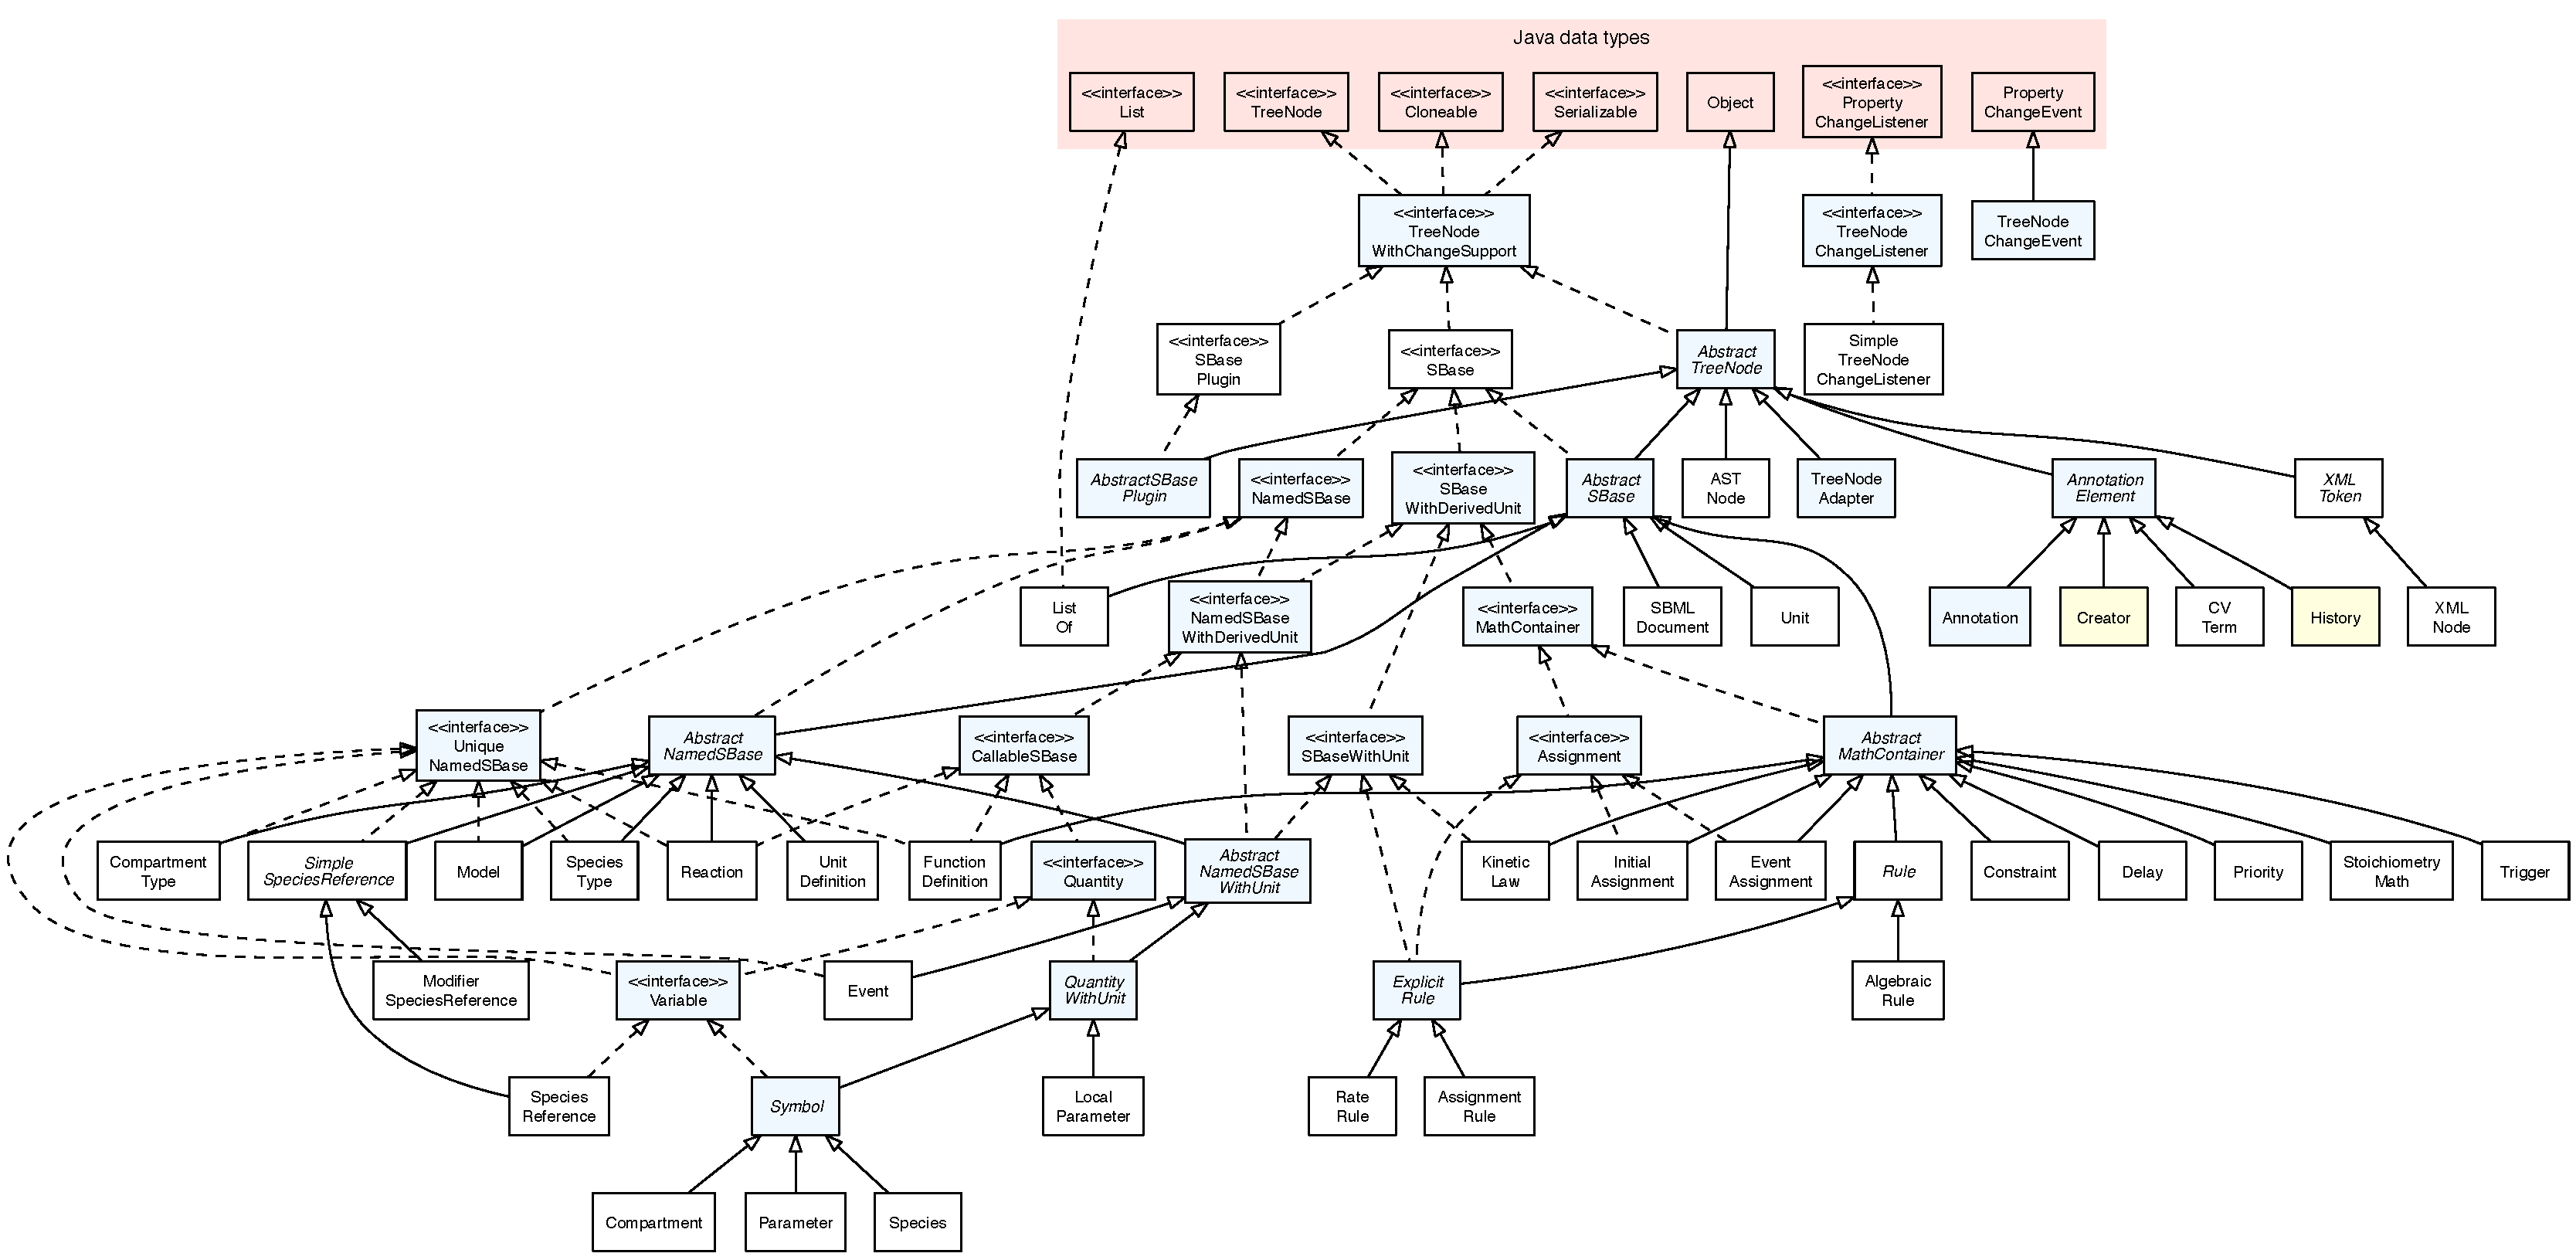
\includegraphics[width=\textwidth]{../img/FullTypeHierarchy.pdf}
\caption[The type hierarchy of the main SBML constructs in JSBML]{The type
hierarchy of the main SBML constructs in JSBML. With letting \texttt{SBase}
extend the interface \texttt{TreeNodeWithChangeSupport} that in turn extends the
Java interfaces \texttt{Cloneable}, \texttt{Serializable}, and
\texttt{TreeNode}, all derived elements of \texttt{SBase} also implement these
types. In this way, derivatives of \texttt{SBase} can be used wherever an
instance of \texttt{TreeNode} is requested. Furthermore, SBML elements that do
not extend \texttt{SBase} are also derived from the identical base type
\texttt{TreeNodeWithChangeSupport}, hence sharing several common methods and
attributes. Elements colored in blue have been introduced as additional, in most
cases abstract, data types in JSBML but do not have a corresponding element in
libSBML. The yellow types \texttt{Creator} and \texttt{History} correspond to
\texttt{ModelCreator} and \texttt{ModelHistory} in libSBML.}
\label{fig:TypeHierarchy}
\end{sidewaysfigure}
\begin{figure}[p]
 \centering
 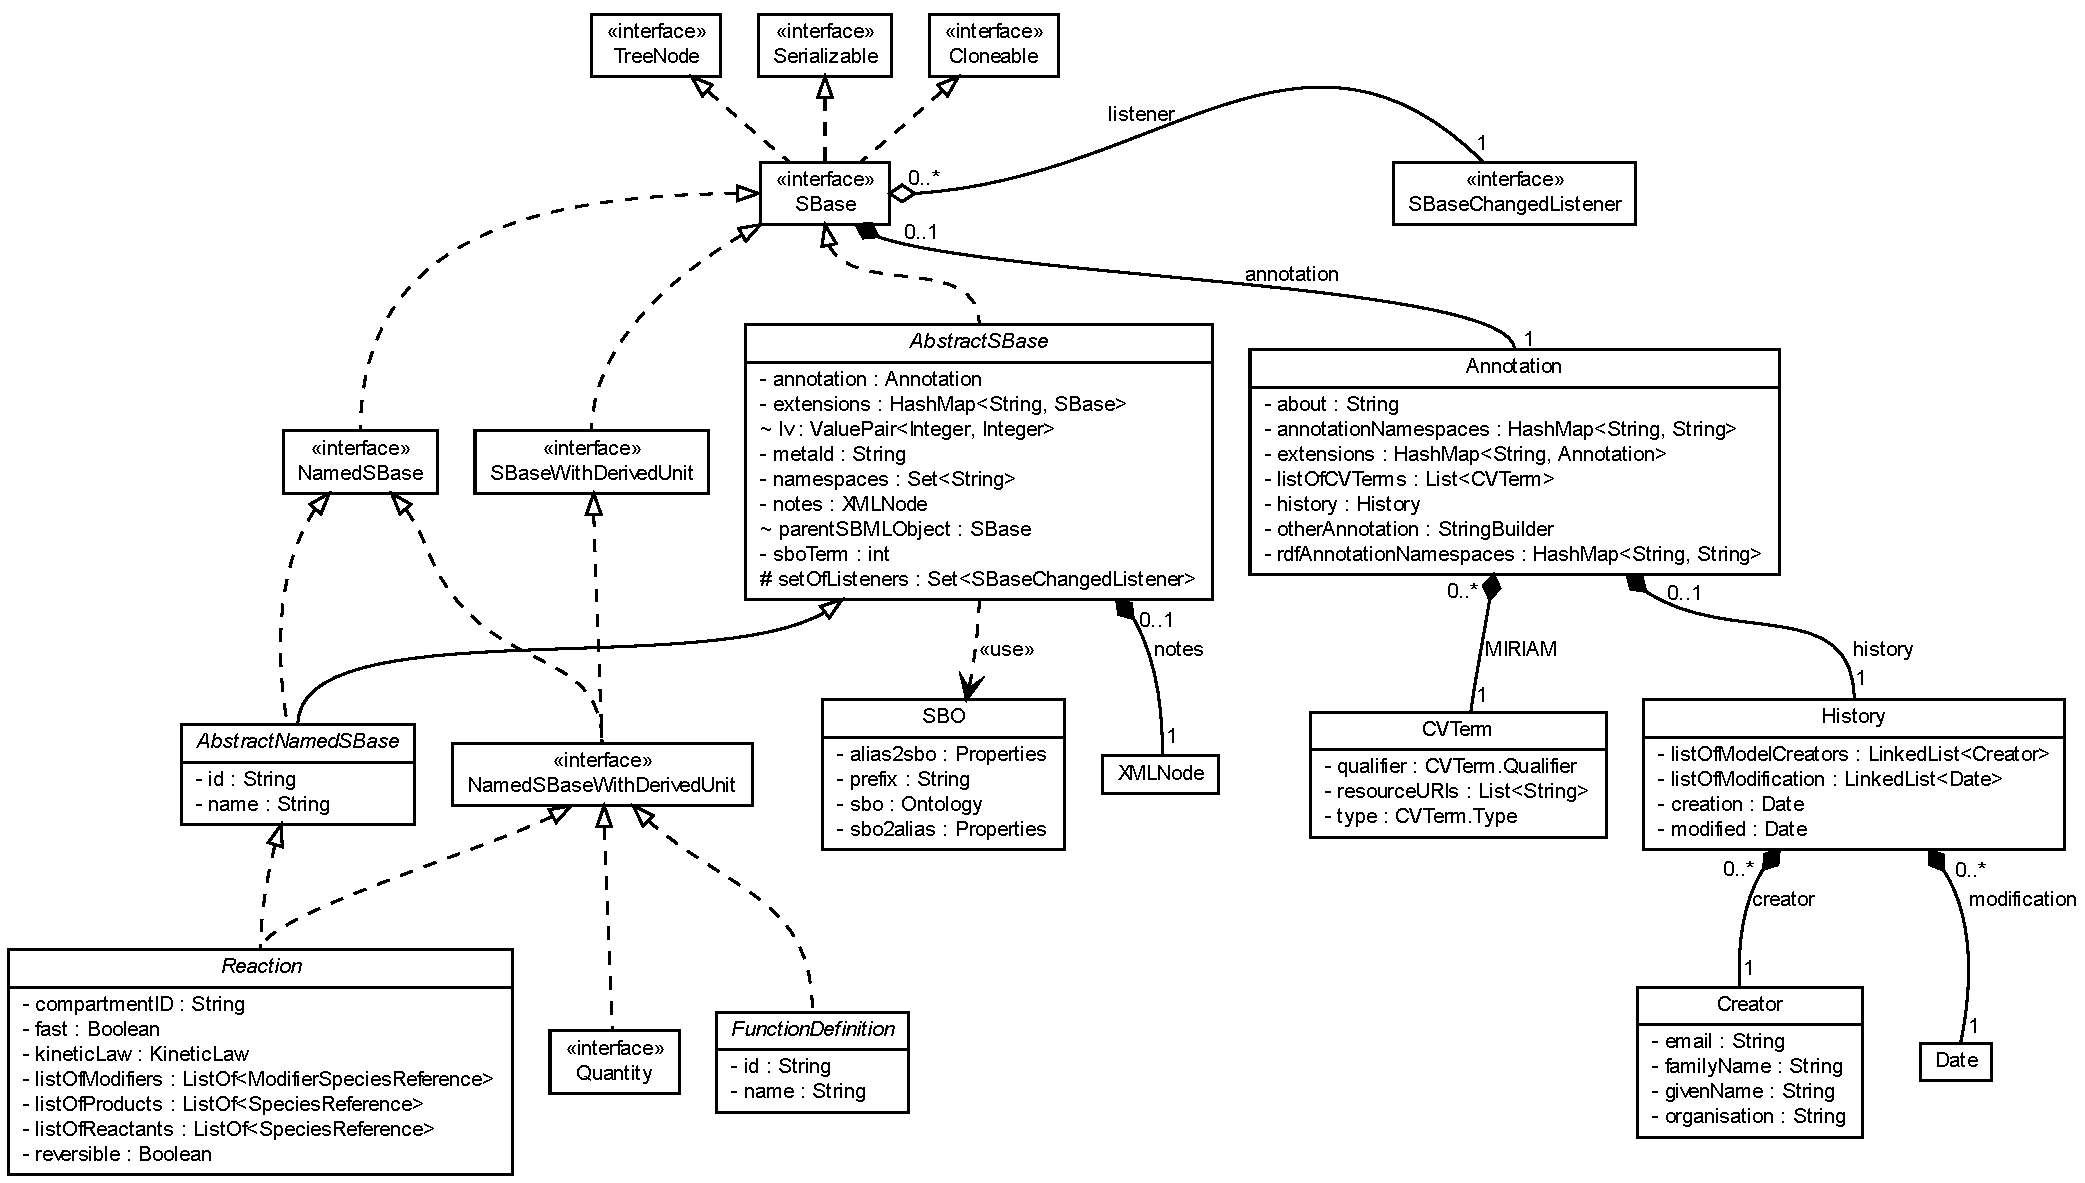
\includegraphics[width=\textwidth]{img/SBase.pdf}
 % SBase.pdf: 1001x568 pixel, 72dpi, 35.31x20.04 cm, bb=0 0 1001 568
 \caption[The interface \texttt{SBase}]{The interface \texttt{SBase}. 
This figure displays the most important top-level data
structures of JSBML with main focus on the differences to libSBML. All data
types that represent SBML constructs in JSBML extend \texttt{AbstractTreeNode}. 
Derivatives of \texttt{SBase} extend either one of the two abstract classes
\texttt{AbstractSBase} or \texttt{AbstractNamedSBase}, which inturn also extend
\texttt{AbstractTreeNode}. The class \texttt{SBO} parses the ontology file
provided on the SBO web site (\url{http://www.ebi.ac.uk/sbo/main/}) in OBO
format (Open Biomedical Ontologies) using a parser provided by the BioJava
project \citep{Holland2008}. For the sake of a clear arrangement, this figure
omits all methods in the UML diagram. \texttt{SBO} stores its ontology in the
classes \texttt{Term} that are interrelated in \texttt{Triples} consisting of
subject, predicate, and object (each being an instance of \texttt{Term}).}
 \label{fig:SBase}
\end{figure}
\begin{figure}[p]
 \centering
 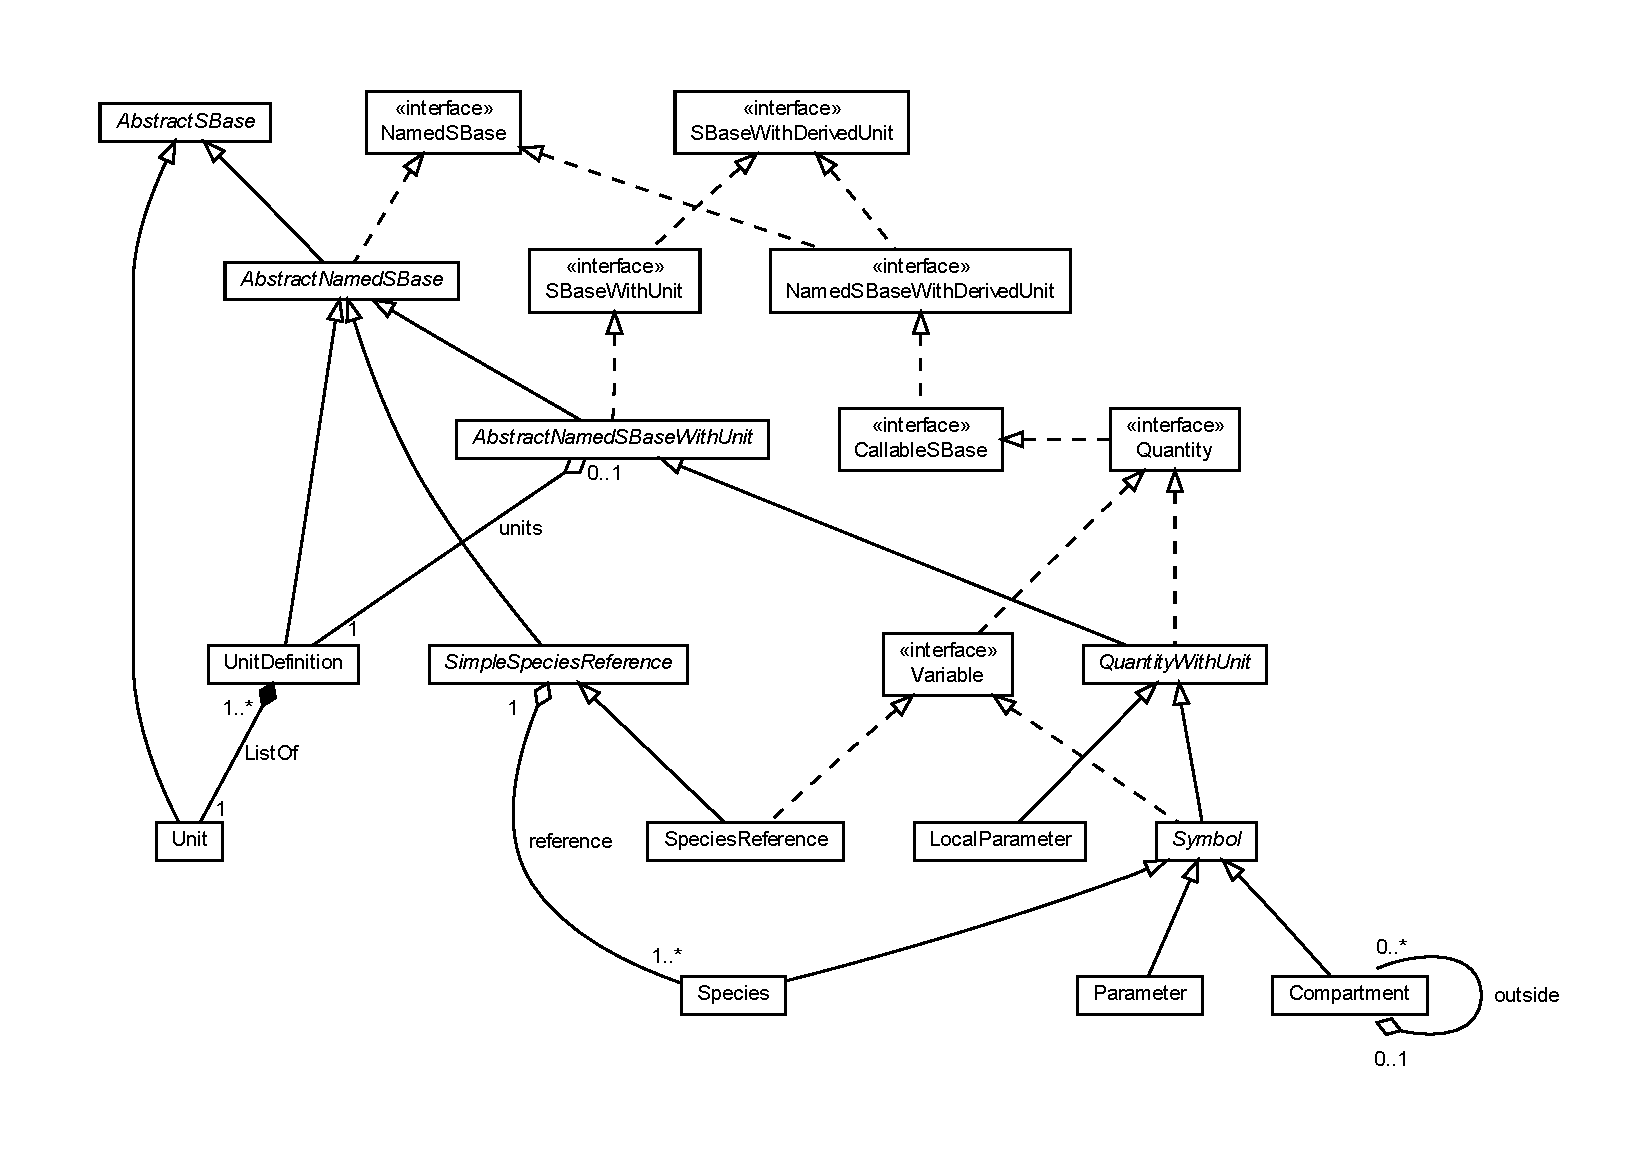
\includegraphics[width=\textwidth]{img/Symbol.pdf}
 % Symbol.pdf: 596x587 pixel, 72dpi, 21.03x20.71 cm, bb=0 0 596 587
 \caption[The interface \texttt{Variable}]{The interface \texttt{Variable}.
 JSBML refers to those components of a model that may change their value during
 a simulation as \texttt{Variable}s. The class \texttt{Symbol} serves as the
 abstract superclass for variables that can also be equipped with a unit.
 Instances of \texttt{Parameter} do not contain any additional field. In
 \texttt{Species}, a Boolean switch decides whether its value is to be
 interpreted as an initial amount or as an initial concentration. In contrast
 to \texttt{Variable}s, \texttt{LocalParameter}s represent constant unit-value
 pairs that can only be accessed within their declaring
 \texttt{KineticLaw}.}
 \label{fig:Variable}
\end{figure}
\begin{figure}[p]
 \centering
 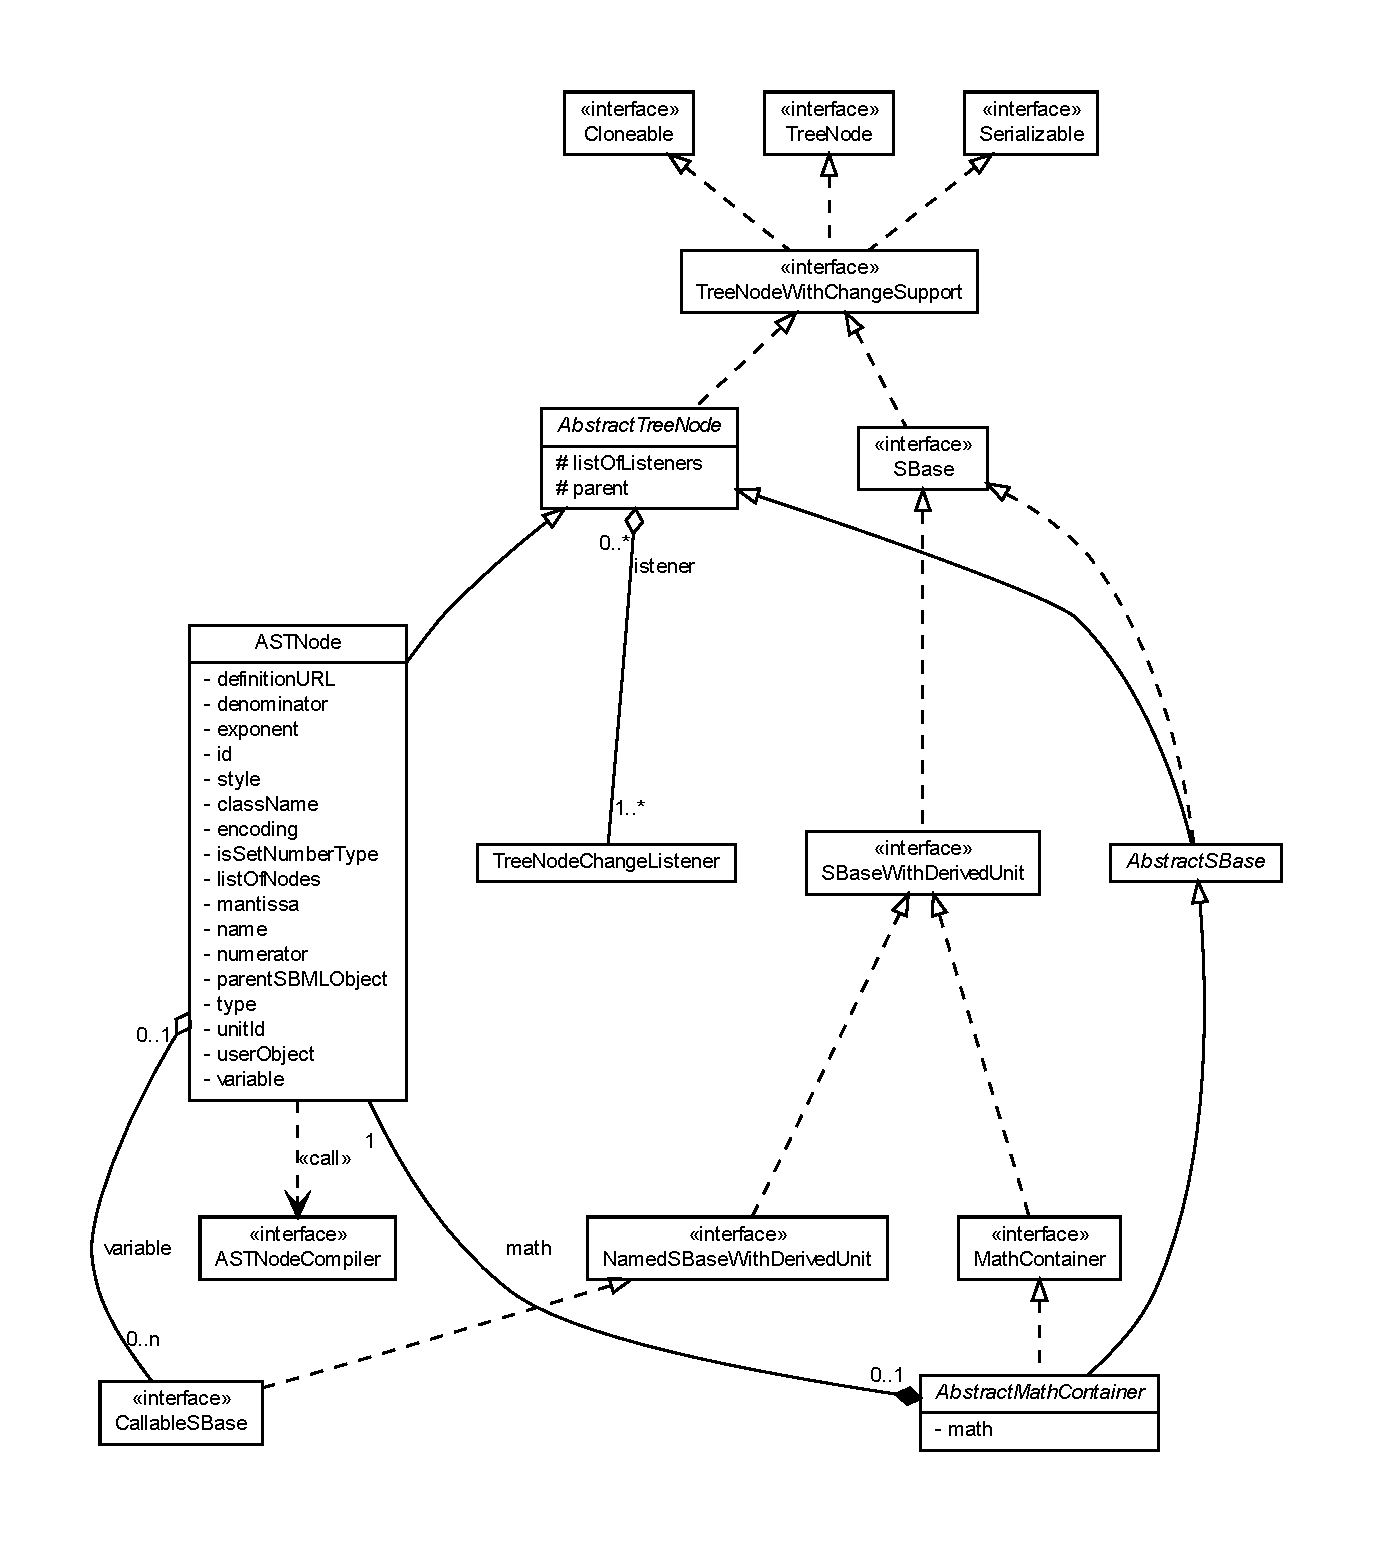
\includegraphics[width=.8\textwidth]{img/ASTNode.pdf}
 % MathContainerClass.pdf: 557x396 pixel, 72dpi, 19.65x13.97 cm, bb=0 0 557 396
 \caption[Abstract syntax trees]{Abstract syntax trees. The class
 \texttt{AbstractMathContainer} serves as the superclass for several model
 components in JSBML. It provides methods to manipulate and access an instance 
 of \texttt{ASTNode}, which can be converted to or read from \texttt{C}-like
 formula \texttt{String}s. Internally, \texttt{AbstractMathContainer}s only
 deal with instances of \texttt{ASTNode}. It should be noted that these
 abstract syntax trees do not implement the \texttt{SBase} interface, but
 extend \texttt{AbstractTreeNode}.}
 \label{fig:MathContainer}
\end{figure}
\begin{sidewaysfigure}[htbp]
 \centering
 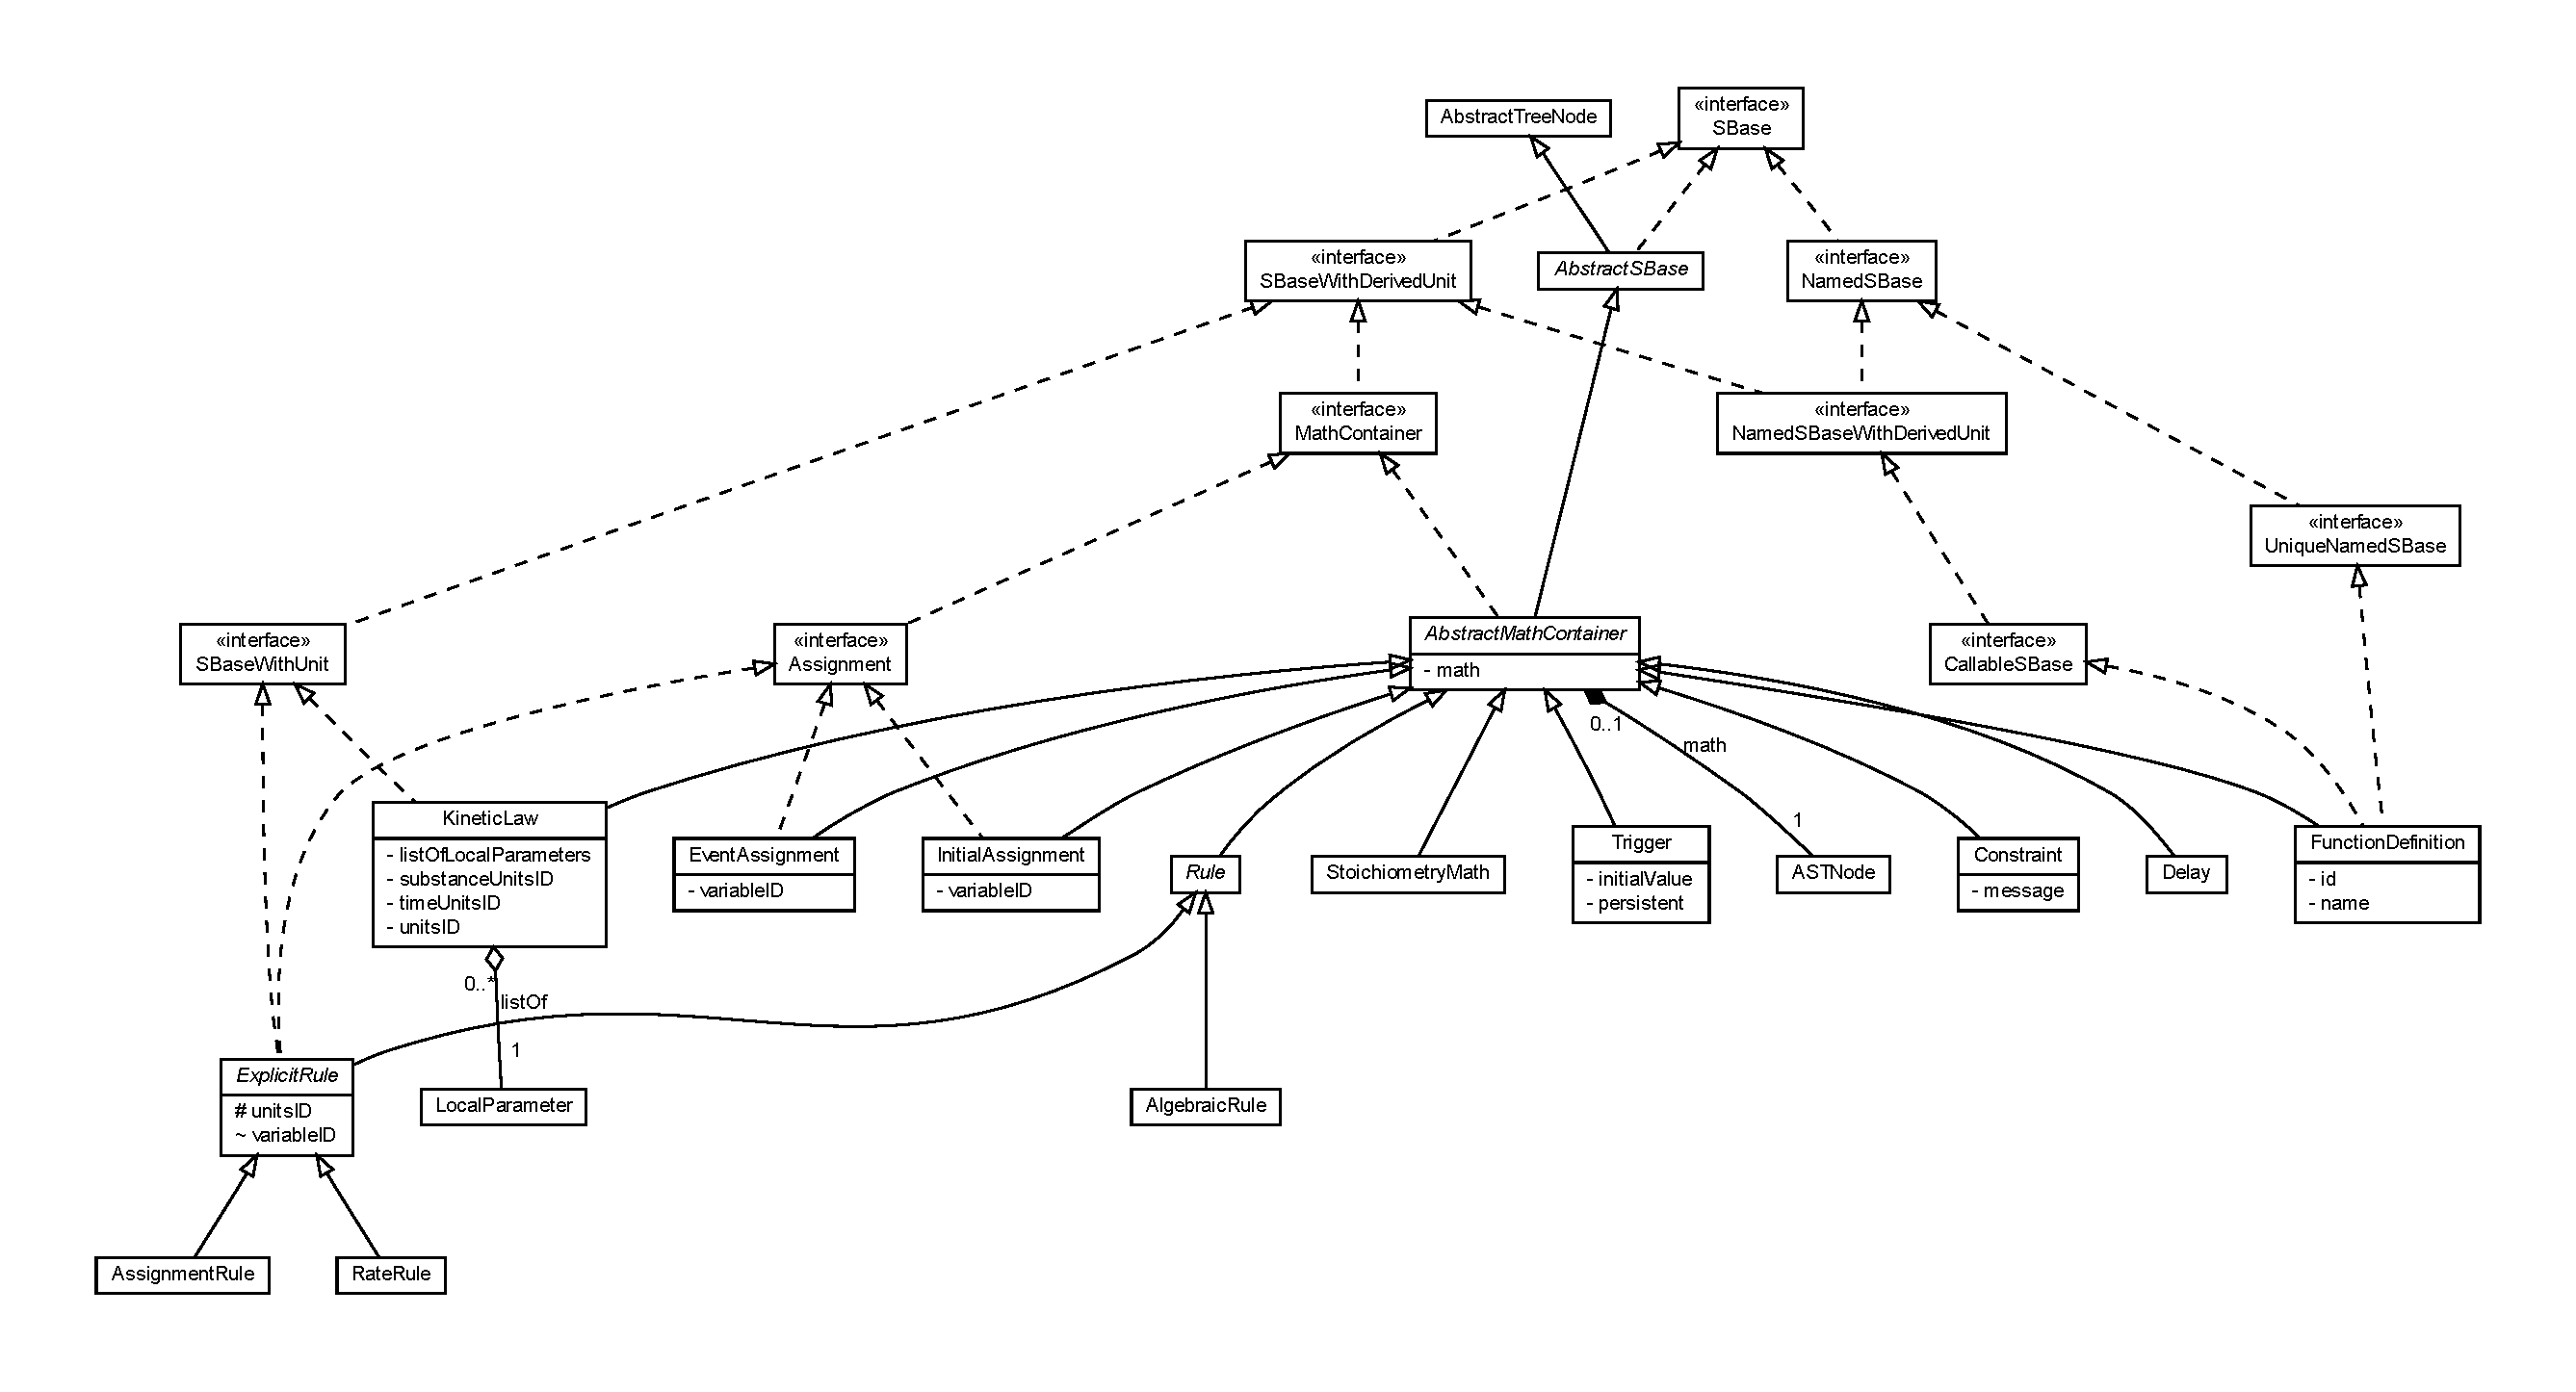
\includegraphics[width=\textwidth]{img/MathContainer.pdf}
 % MathContainerClass.pdf: 557x396 pixel, 72dpi, 19.65x13.97 cm, bb=0 0 557 396
 \caption[Containers for mathematical expressions]{Containers for mathematical
 expressions. The interface \texttt{MathContainer}, particularly
 its directly derived class \texttt{AbstractMathContainer}, constitutes the
 superclass for all elements that store and manipulate mathematical formulas in
 JSBML, which is done in form of \texttt{ASTNode} objects. These can be
 evaluated using an implementation of \texttt{ASTNodeCompiler}. Note that some
 classes that extend \texttt{AbstractMathContainer} do not contain any own
 fields or methods: \texttt{Delay}, \texttt{Priority},
 \texttt{StoichiometryMath}, or \texttt{AlgebraicRule}.}
 \label{fig:MathContainerHierarchy}
\end{sidewaysfigure}
Whenever multiple elements defined in at least one of the SBML
\index{SBML}%
specifications
\index{SBML!specification}%
share some attributes, JSBML
\index{JSBML!type hierarchy}%
provides a common superclass or at least a common interface that gathers methods
for the manipulation of the shared properties. In this way, the type hierarchy
of JSBML
\index{application programming interface!JSBML}%
has become quite complex (see
Figs.~\vrefrange{fig:TypeHierarchy}{fig:MathContainerHierarchy}). Just as in
libSBML,
\index{application programming interface!libSBML}%
all elements extend the abstract type \texttt{SBase},
\index{SBase@\texttt{SBase}}%
but in JSBML, \texttt{SBase} has become an interface. This allows more complex
relations between derived data types. In contrast to libSBML, \texttt{SBase} in
JSBML extends the interface \texttt{TreeNodeWithChangeSupport}%
\index{TreeNodeWithChangeSupport@\texttt{TreeNodeWithChangeSupport}} 
that in turn extends three other interfaces: \texttt{Cloneable},
\texttt{Serializable}, \index{Serializable@\texttt{Serializable}}% and \texttt{TreeNode}. As all elements defined in JSBML
\index{cloning}%
override the \texttt{clone()} method from the class \texttt{java.lang.Object},
\index{Object@\texttt{Object}}%
all JSBML elements can be deeply copied and are therefore \emph{clone-able}. By
extending the interface \texttt{Serializable},
\index{Serializable@\texttt{Serializable}}%
it is possible to store JSBML
\index{application programming interface!JSBML}%
elements in binary form without explicitly writing them to an SBML file.
\index{SBML!XML file}%
In this way, programs can easily load and save their in-memory objects or send
complex data structures through a network connection without the need of
additional file encoding and subsequent parsing. The third interface,
\texttt{TreeNode}%
\index{TreeNode@\texttt{TreeNode}} 
is actually defined in Java's \texttt{swing}
\index{graphical user interface!\texttt{swing}}%
package.
\texttt{TreeNode} is a type that is independent of any graphical information. It
basically defines recursive methods on hierarchically structured data types,
such as iteration over all of its successors. In this way, all instances of
JSBML's \texttt{SBase}\index{SBase@\texttt{SBase}}%
interface can be directly passed to the \texttt{swing}
\index{graphical user interface!\texttt{swing}}%
class \texttt{JTree}
\index{graphical user interface!\texttt{JTree}}%
and can hence be easily visualized. Listing~\vref{lst:Visualization}
demonstrates in a simple code example how to parse an SBML file
\index{SBML!XML file}%
and to immediately display its content on a \texttt{JFrame}.
\index{graphical user interface!\texttt{JFrame}}%
\ifthenelse{\boolean{includeCodeExample}}{%
  \lstinputlisting[language=Java,float,caption={Parsing and visualizing the
  content of an SBML file},label=lst:Visualization]{%
../posters/2010_ICSB_and_COMBINE/org/sbml/gui/JSBMLvisualizer.java}
  Fig.~\vref{fig:Visualization} shows an example output when applying the
  program to an SBML test model\index{SBML!Test cases}.
  \begin{SCfigure}[][t]
  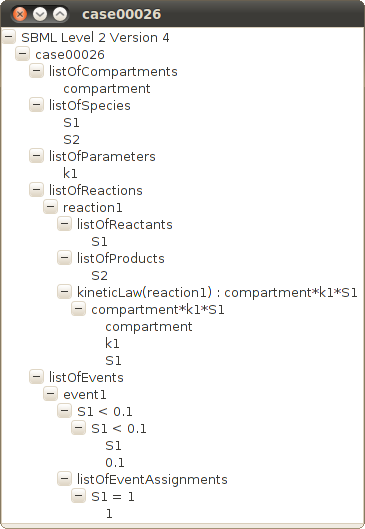
\includegraphics[width=.35\textwidth]{%
../posters/2010_ICSB_and_COMBINE/JSBMLvisualizerTransparent}
  \caption[Tree representation of an SBML file]{A tree representation of the
    content of SBML test model \texttt{case00026}. In JSBML, the hierarchically
    structured \texttt{SBMLDocument} can be traversed recursively because all
    instances of \texttt{SBase} implement the interface \texttt{TreeNode}.}
  \label{fig:Visualization}
  \end{SCfigure}
}{%
}%
The \texttt{ASTNode} class in JSBML\index{ASTNode@\texttt{ASTNode}} is also
derived from all these three interfaces and can hence be cloned, serialized, and
visualized in the same way.

However, it is important to note that JSBML does not depend on any particular
graphical user interface because no other classes from \texttt{swing} are
initialized when loading the interface
\texttt{TreeNode}\index{TreeNode@\texttt{TreeNode}}.

\subsection{\texttt{AbstractTreeNode}}%
\index{TreeNode!AbstractTreeNode@\texttt{AbstractTreeNode}}

When looking at the SBML specification, one may notice that SBML defines a data
structure in an an entirely tree-based manner. Besides
\texttt{SBase}\index{SBase@\texttt{SBase}}, SBML contains also other kinds of
tree nodes that are hierarchically linked within the \texttt{SBMLDocument}. 
In order to unify the programming interface, JSBML defines abstract data types
as top-level ancestors for its \texttt{SBase} implementation as well as all
other hierarchical elements, such as \texttt{Annotation},
\texttt{ASTNode}\index{ASTNode@\texttt{ASTNode}},
\texttt{Creator}\index{annotation!Creator@\texttt{Creator}},
\texttt{CVTerm}\index{annotation!CVTerm@\texttt{CVTerm}},
\texttt{History}\index{annotation!History@\texttt{History}}, and
\texttt{XMLNode}\index{XML!XMLNode@\texttt{XMLNode}} (for notes in
XHTML\index{XHTML} format).

First, the interface \texttt{TreeNodeWithChangeSupport}%
\index{TreeNodeWithChangeSupport@\texttt{TreeNodeWithChangeSupport}}
defines a \emph{cloneable} and \emph{serializable} version of
\texttt{TreeNode}. In addition, it also provides methods to notify dedicated
\texttt{TreeNodeChangeListener}s%
\index{TreeNodeChangeListener@\texttt{TreeNodeChangeListener}}
about any changes within the data structure.

Its abstract implementation, \texttt{AbstractTreeNode}, does already implement
many of the methods inherited from \texttt{TreeNodeWithChangeSupport} and also
maintains a list of \texttt{TreeNodeChangeListener}s. Furthermore, this class
contains a basic implementation of the methods \texttt{equals} and
\texttt{hashCode}, which both already make use of a recursive call over all
descendants within the hierarchical SBML data structure. Based on this class,
the implementation of all derived data types has become much simpler. The
abstract implementation of \texttt{SBase} is also an instance of
\texttt{AbstractTreeNode}.


\subsection{Characteristic features of \texttt{SBase}s}

The SBML\index{SBML} specifications define the data type
\texttt{SBase}\index{SBase@\texttt{SBase}}\index{SBML!specification} as the
supertype for all other SBML elements. In JSBML, \texttt{SBase} has become an
interface and most elements therefore extend its abstract implementation
\texttt{AbstractSBase}\index{SBase@\texttt{SBase}!\texttt{AbstractSBase}}.

In contrast to libSBML, the Level and Version of such an \texttt{AbstractSBase}
is stored in a special generic object, a \texttt{ValuePair}.
\index{JSBML!ValuePair@\texttt{ValuePair}}%
The class \texttt{ValuePair} takes two values of any type that both implement
the interface \texttt{Comparable}.
\index{Comparable@\texttt{Comparable}}%
Storing the Level/Version combination in such a \texttt{ValuePair}, which itself
implements the \texttt{Comparable} interface, allows users to perform checks for
an expected Level/Version combination of an element more easily, as the example
in Listing~\vref{lst:LevelVersionCheck} demonstrates.
\begin{lstlisting}[language=Java,float=h,caption={Check for a minimal expected Level/Version combination},label={lst:LevelVersionCheck}]
if (mySBase.getLevelAndVersion().compareTo(Integer.valueOf(2),
        Integer.valueOf(2)) < 0) {
  throw new IllegalArgumentException(String.format(
          "Cannot create a %s with Level = %s and Version = &s.",
          mySBase.getElementName(), getLevel(), getVersion()));
}
\end{lstlisting}
The method \texttt{getLevelAndVersion()} in \texttt{AbstractSBase}
\index{SBase@\texttt{SBase}!\texttt{AbstractSBase}}%
delivers an instance of \texttt{ValuePair}
\index{JSBML!ValuePair@\texttt{ValuePair}}%
with the Level and Version combination for the respective element.

Some types derived from \texttt{SBase} contain an identifier, a so-called
\texttt{id}. JSBML gathers all these elements under the common interface
\texttt{NamedSBase}. The class \texttt{AbstractNamedSBase}, which extends
\texttt{AbstractSBase}, implements this interface.
\index{SBase@\texttt{SBase}!\texttt{NamedSBase}}%
\index{SBase@\texttt{SBase}!\texttt{AbstractNamedSBase}}%
The interface \texttt{UniqueNamedSBase} markes all those elements whose
identifier must be unique within the model, i.e., no other element within the
model may have the same identifier. The identifiers of all instances of
\texttt{NamedSBase} must be unique if these are defined. The Boolean method
\texttt{isIdMandatory()} in \texttt{NamedSBase} indicates if an identifier must
be defined for an element in order to create a valid SBML data structure. The
only two elements with not-unique identifiers are
\texttt{UnitDefinition}s\index{unit!UnitDefinition@\texttt{UnitDefinition}},
whose identifiers exist in a separate namespace, and
\texttt{LocalParameter}s\index{parameter!LocalParameter@\texttt{LocalParameter}},
whose identifiers may shaddow the identifiers of global elements.

Many SBML elements represent some quantitative value, which is associated with a
unit. However, the value does not necessarily have to be defined explicitly. In
many cases, it needs to be computed from a formula contained in the instance of
\texttt{SBase} in form of an abstract syntax tree, i.e., \texttt{ASTNode}.
\index{ASTNode@\texttt{ASTNode}}%
Therefore, also the associated unit may not be set explicitly but can be derived
when evaluating the formula. In JSBML, the interface
\texttt{SBaseWithDerivedUnit}
\index{SBase@\texttt{SBase}!\texttt{SBaseWithDerivedUnit}}%
unifies all those elements
that either explicitly or implicitly contain some unit. If these elements can
also be addressed using an identifier, they also implement the interface
\texttt{NamedSBaseWithDerivedUnit}.
\index{SBase@\texttt{SBase}!\texttt{NamedSBaseWithDerivedUnit}}%
Within formulas, i.e., \texttt{ASTNode}s,
references can only be made to instances of \texttt{CallableSBase},
\index{JSBML!CallableSBase@\texttt{CallableSBase}}%
which is a special case of \texttt{NamedSBaseWithDerivedUnit}.
Fig.~\vref{fig:Variable} shows this part of JSBML's type hierarchy in more
detail.

As a special case, these elements may explicitly declare a unit. The interface
\texttt{SBaseWithUnit}
\index{SBase@\texttt{SBase}!\texttt{SBaseWithUnit}}%
serves as the supertype for all those elements that may
be explicitly equipped with a unit. The convenient class
\texttt{AbstractNamedSBaseWithUnit}
\index{SBase@\texttt{SBase}!\texttt{AbstractNamedSBaseWithUnit}}%
\index{SBase@\texttt{SBase}!\texttt{AbstractNamedSBase}}%
extends \texttt{AbstractNamedSBase} and
implements both interfaces \texttt{SBaseWithUnit} and
\index{SBase@\texttt{SBase}!\texttt{SBaseWithUnit}}%
\texttt{NamedSBaseWithDerivedUnit}.
\index{SBase@\texttt{SBase}!\texttt{NamedSBaseWithDerivedUnit}}%
All elements derived from this abstract class may therefore declare a unit and
can be addressed using an unambiguous identifier.

Furthermore, the interface \texttt{Quantity}
\index{JSBML!quantity@\texttt{Quantity}}%
describes an element that is associated with a value and at least a derived
unit. In addition, a \texttt{Quantity} can be addressed
using its unambiguous identifier. JSBML uses the term \texttt{QuantityWithUnit}
for a \texttt{Quantity} that explicitly declares its unit. In contrast to
\texttt{Quantity} that explicitly declares its unit. In contrast to
\texttt{Quantity}, the data type \texttt{QuantityWithUnit}
\index{JSBML!quantityWithUnit@\texttt{QuantityWithUnit}}%
is not an interface, but an abstract class.

If a \texttt{Quantity} provides a Boolean
\index{Boolean}%
switch to decide whether it describes a constant,
\index{constant}%
JSBML represents such a type in the interface \texttt{Variable}.
\index{JSBML!variable@\texttt{Variable}}%
Finally, JSBML refers to \texttt{Variable}s with a defined unit as a
\texttt{Symbol}
\index{JSBML!symbol@\texttt{Symbol}}%
and provides a corresponding abstract class. In this way, the
SBML elements \texttt{Compartment}, \texttt{Parameter}, and \texttt{Species}
\index{compartment!\texttt{Compartment}}%
\index{parameter!\texttt{Parameter}}%
\index{species!\texttt{Species}}%
are special cases of \texttt{Symbol} in JSBML. The specification of SBML Level~3
\index{SBML!Level~3}%
introduces another type of \texttt{Variable}, which does not explicitly declare
its unit: \texttt{SpeciesReference}. On the other hand, a
\texttt{LocalParameter}
\index{parameter!\texttt{LocalParameter}}%
is a \texttt{QuantityWithUnit},
\index{JSBML!quantityWithUnit@\texttt{QuantityWithUnit}}%
but not a \texttt{Variable}, because it is always constant.
\index{constant}%


\subsection{The \texttt{MathContainer} interface}

This interface gathers all those elements that may contain mathematical
expressions encoded in abstract syntax trees (instances of
\texttt{ASTNode}\index{ASTNode@\texttt{ASTNode}}).
The abstract class \texttt{AbstractMathContainer}
\index{JSBML!MathContainer@\texttt{MathContainer}}%
serves as actual superclass
for the majority of the derived types.
Figs.~\vrefrange{fig:MathContainer}{fig:MathContainerHierarchy} give a better
overview of how this data structure is intended to function.


\subsection{The \texttt{Assignment} interface}

JSBML
\index{JSBML!assignment@\texttt{Assignment}}%
unifies all those elements that may
change the value of some \emph{variable} in SBML\index{SBML} under the interface
\texttt{Assignment}. This interface uses the term \emph{variable}
for the element whose value is to be changed
depending on some mathematical expression that is also present in the
\texttt{Assignment} (because \texttt{Assignment} extends the interface
\texttt{MathContainer}).
\index{JSBML!MathContainer@\texttt{MathContainer}}%
Therefore,
an \texttt{Assignment} contains methods such as
\texttt{set}-/\texttt{getVariable(Variable v)} and also \texttt{isSetVariable()}
as well as \texttt{unsetVariable()}. In addition to that, JSBML also provides
the methods \texttt{set}-/\texttt{getSymbol(String symbol)} in the
\texttt{InitialAssignment}
\index{InitialAssignment@\texttt{InitialAssignment}}%
class to make sure that switching from libSBML
to JSBML is quite smoothly.
However, the preferred way in JSBML
\index{JSBML!variable@\texttt{Variable}}%
is to apply the methods \texttt{setVariable} either with \texttt{String}
\index{String@\texttt{String}!identifier}%
or \texttt{Variable} instances as arguments.
Fig.~\vref{fig:MathContainerHierarchy} displays the type hierarchy of the
\texttt{Assignment} interface in more detail.



\section{Differences in the abstract programming interface}

JSBML strives to attain an almost complete compatibility to libSBML. However,
the differences in the programming languages \texttt{C++}
\index{C++@\texttt{C++}}%
and Java\texttrademark{} lead to the necessity of introducing some differences.
In some cases, a direct ``translation" from \texttt{C++} and \texttt{C} code to
\index{C@\texttt{C}}%
Java would not be very elegant. JSBML wants to provide a Java API,
\index{application programming interface!Java}%
whose classes and methods are structured, named, and behave like classes and
methods in other Java libraries. In this section, we will discuss the most
important differences in the APIs of JSBML
\index{application programming interface!JSBML}%
and libSBML.
\index{application programming interface!libSBML}%


\subsection{Abstract syntax trees}

Both libraries define a class \texttt{ASTNode}\index{ASTNode@\texttt{ASTNode}}
for in-memory manipulation and evaluation of abstract syntax trees that represent
mathematical formulas and equations. These can either be parsed from a representation in \texttt{C}
language-like \texttt{String}s\index{String@\texttt{String}!formula}, or from a MathML\index{MathML} representation. The JSBML\index{ASTNode@\texttt{ASTNode}}
\texttt{ASTNode} provides various methods to transform these trees to other
formats, for instance, \LaTeX{}
\index{LaTeX@\LaTeX} \texttt{String}s. In JSBML, several static
methods allow easy creation of new syntax trees, for instance, the following
code
\begin{lstlisting}[language=Java,numbers=none]
ASTNode myNode = ASTNode.plus(myLeftAstNode, myRightASTNode);
\end{lstlisting}
creates a new instance of \texttt{ASTNode} which represents the sum of the two
other \texttt{ASTNode}s. In this way, even complex trees can be easily
manipulated.

In SBML, abstract syntax trees may refer to the following elements:
\texttt{Parameter}s, \texttt{LocalParameter}s, \texttt{FunctionDefinition}s,
\texttt{Reaction}s, \texttt{Compartment}s, \texttt{Species}, and, since Level~3,
also \texttt{SpeciesReference}s. JSBML gathers all these elements under the
common interface \texttt{CallableSBase},
\index{JSBML!CallableSBase@\texttt{CallableSBase}}%
\index{SBase@\texttt{SBase}!CallableSBase@\texttt{CallableSBase}}%
which extends the interface \texttt{NamedSBaseWithDerivedUnit}.
\index{JSBML!NamedSBaseWithDerivedUnit@\texttt{NamedSBaseWithDerivedUnit}}%
\index{SBase@\texttt{SBase}!%
NamedSBaseWithDerivedUnit@\texttt{NamedSBaseWithDerivedUnit}}%
In this way, JSBML ensures that only identifiers of those elements can be set in
instances of \texttt{ASTNode}.
\index{ASTNode@\texttt{ASTNode}}%
JSBML provides a set of convenient constructors and methods to work with
instances of \texttt{CallableSBase},
\index{JSBML!CallableSBase@\texttt{CallableSBase}}%
\index{SBase@\texttt{SBase}!CallableSBase@\texttt{CallableSBase}}%
of which we here give a short overview.
\begin{lstlisting}[language=Java,numbers=none,float=h,captionpos=t,
title={Getter and setter:}]
public void setVariable(CallableSBase variable) { ... }

public CallableSBase getVariable() { ... }
\end{lstlisting}
The set method allows users to change the type of an \texttt{ASTNode} to
\texttt{ASTNode.Type.NAME}
\index{ASTNode@\texttt{ASTNode}!ASTNode.Type@\texttt{ASTNode.Type}}%
and to directly set the name to the identifier of the
given \texttt{CallableSBase}.
\index{JSBML!CallableSBase@\texttt{CallableSBase}}%
\index{SBase@\texttt{SBase}!CallableSBase@\texttt{CallableSBase}}%
The \texttt{get} method directly looks for the corresponding element in the
\texttt{Model}\index{model!Model@\texttt{Model}}%
and returns this element. If no such element can be found or the type of the
\texttt{ASTNode} is something different from \texttt{ASTNode.Type.NAME}, an
\index{ASTNode@\texttt{ASTNode}!ASTNode.Type@\texttt{ASTNode.Type}}%
\index{ASTNode@\texttt{ASTNode}}%
exception will be thrown.

\begin{lstlisting}[language=Java,numbers=none,float=h,captionpos=t,
title={Some examples for convenient manipulation methods, of which some are static:}]
public static ASTNode frac(MathContainer container,
      CallableSBase numerator, CallableSBase denominator) {...}

public static ASTNode pow(MathContainer container,
      CallableSBase basis, CallableSBase exponent) { ... }

public ASTNode plus(CallableSBase nsb) { ... }
\end{lstlisting}
Methods like these above facilitate creating or manipulating complex abstract
syntax trees. Several static methods are available that directly create small
trees from given elements in memory, whereas some methods such as the
\texttt{plus} method changes the structure of existing syntax trees.

\begin{lstlisting}[language=Java,numbers=none,float=h,captionpos=t,
title={Some examples for convenient constructors:}]
public ASTNode(CallableSBase nsb) { ... }

public ASTNode(CallableSBase nsb, MathContainer parent) { ... }
\end{lstlisting}
With these constructors, dedicated single nodes can be created whose type
(from the enumeration \texttt{ASTNode.Type}) will be \texttt{NAME}
\index{ASTNode@\texttt{ASTNode}!ASTNode.Type@\texttt{ASTNode.Type}}%
and whose name will be set to the identifier of the given
\texttt{CallableSBase}.
\index{JSBML!CallableSBase@\texttt{CallableSBase}}%
\index{SBase@\texttt{SBase}!CallableSBase@\texttt{CallableSBase}}%


\subsection{The \texttt{ASTNodeCompiler} class}

This interface allows users to create customized interpreters for the
content of mathematical equations encoded in abstract syntax trees. It
is directly and recursively called from the \texttt{ASTNode} class and returns
an \texttt{ASTNodeValue}
\index{ASTNode@\texttt{ASTNode}!\texttt{ASTNodeValue}}%
\index{ASTNode@\texttt{ASTNode}!\texttt{ASTNodeCompiler}}%
object, which wraps the possible evaluation results of the interpretation.
JSBML\index{ASTNode@\texttt{ASTNode}} already provides several implementations of this
interface, for instance, \texttt{ASTNode} objects can be directly translated to
\texttt{C} language-like \texttt{String}s\index{String@\texttt{String}!formula},
\LaTeX,\index{LaTeX@\LaTeX} or MathML\index{MathML} for further processing.
Furthermore, the class \texttt{UnitsCompiler},
\index{unit!UnitsCompiler@\texttt{\texttt{UnitsCompiler}}}%
which JSBML uses to derive the unit of an abstract syntax tree, also implements
this interface.

\subsection{Cloning when adding child nodes to instances of \texttt{SBase}}

When adding elements such as a \texttt{Species}
\index{species!\texttt{Species}}%
to a \texttt{Model}\index{model!\texttt{Model}}, libSBML\index{cloning} will
clone the object and add the clone to the \texttt{Model}. In contrast,
JSBML\index{cloning} does
not automatically perform cloning. The advantage is that modifications on the
object belonging to the original pointer will also propagate to the element
added to the \texttt{Model}. Furthermore, this is more efficient with respect to
the run time and also more intuitive for Java programmers. If cloning is
necessary, users should call the \texttt{clone()} method manually. Since all
instances of \texttt{SBase}\index{SBase@\texttt{SBase}} and also
\texttt{Annotation}\index{annotation},
\texttt{ASTNode}\index{ASTNode@\texttt{ASTNode}},
\texttt{CVTerm}\index{annotation!\texttt{CVTerm}}, and
\texttt{History}\index{annotation!\texttt{History}} extend
\texttt{AbstractTreeNode}\index{AbstractTreeNode@\texttt{AbstractTreeNode}},
which inturn implements the interface \texttt{Cloneable}\index{cloning} (see
Fig.~\vref{fig:TypeHierarchy}), all these elements can be naturally cloned.
However, when cloning an object in JSBML\index{cloning}, such as an
\texttt{AbstractNamedSBase},
\index{SBase@\texttt{SBase}!\texttt{AbstractNamedSBase}}
% all children of this element will recursively be cloned before adding them to
% the new element. This is necessary, because the data structures specified in
% SBML \index{SBML!hierarchical structure}
define a tree, in which each element has exactly one parental node.

\subsection{Deprecation}

The intention of JSBML\index{JSBML!deprecation} is to provide a Java library
that supports the latest specifications of SBML\index{SBML}.
\index{SBML!specification}%
\index{deprecation}%
But we also want to support earlier specifications. So JSBML provides methods
and classes to cover elements and properties from earlier SBML specifications as
well, but these are often marked as being deprecated to avoid creating models
that refer to these elements. Furthermore, JSBML contains many methods just for
compatibility with libSBML, for instance, a method such as \texttt{getNumXyz()}
is not considered to be very Java-like, but very common
\texttt{C++}\index{C++@\texttt{C++}} programming style. Usually, Java
programmers would expect the method being called \texttt{getXyzCount()}
instead. In cases like this, JSBML provides alternative methods and marks these
methods that originate from libSBML as deprecated.


\subsection{Compartments}

In SBML Level 3
\index{SBML!Level~3}%
\citep{Hucka2010a}, the domain of the \texttt{spatialDimensions} attribute in
\texttt{Compartment}s was changed from $\lbrace 0, 1, 2, 3\rbrace$, which can be
represented with a \texttt{short} value in Java, to a value in $\mathbb{R}$,
i.e., a \texttt{double} value. For this reason, the method
\texttt{getSpatialDimensions()} in JSBML
always returns a \texttt{double} value. For consistency with libSBML, the
\texttt{Compartment} class in JSBML also provides the redundant method
\texttt{getSpatialDimensionsAsDouble()} that returns the identical value, but
that is marked as a deprecated method.
\index{compartment}%
\index{compartment!\texttt{getSpatialDimensions()}}%
\index{compartment!\texttt{getSpatialDimensionsAsDouble()}}%


\subsection{Exceptions}

In case of an error, JSBML
\index{exception}%
throws often an exception while libSBML\index{exception!error codes} methods
return some error codes instead. This behavior helps programmers and users to
avoid creating invalid SBML data structures already when dealing with these in
memory. Furthermore, exception handling is very well implemented in Java and it
is therefore a better programming style in this language. Methods can already
declare that these may potentially throw exceptions. In this way, programmers
can be aware of potential sources of problems already at the time of writing the
source code. Examples are the \texttt{ParseException}
\index{exception!\texttt{ParseException}}%
that may be thrown if a given formula cannot be parsed properly into an
\texttt{ASTNode}
\index{ASTNode@\texttt{ASTNode}}%
data structure, or \texttt{InvalidArgumentException}s
\index{exception!\texttt{InvalidArgumentException}}%
if inappropriate values are passed to methods. For instance,
\begin{itemize}
 \item An object representing a constant\index{constant} such as a
 \texttt{Parameter} whose \texttt{constant} attribute has been set to
\texttt{true} cannot be used as the \texttt{Variable} element in an
\texttt{Assignment}.
\index{JSBML!assignment@\texttt{Assignment}}%
\index{JSBML!variable@\texttt{Variable}}%
\index{parameter!\texttt{Parameter}}%
\index{parameter!\texttt{constant}}%
 \item An instance of \texttt{Priority}\index{event!\texttt{Priority}} can only
 be assigned to an \texttt{Event}s\index{event!\texttt{Event}} if its
 \texttt{level}\index{SBML!Level~3} attribute has at least been set to
 three.\index{SBase@\texttt{SBase}!\texttt{AbstractNamedSBase}}
 \item Another example is the \texttt{InvalidArgumentException} that
 is thrown when trying to set an invalid identifier \texttt{String} for an
 instance of \texttt{AbstractNamedSBase}.
 \item JSBML keeps track of all identifiers within a model. For each namespace
 it contains a separate set of identifiers within the
 \texttt{Model}\index{Model@\texttt{Model}}. It is therefore not possible to
 assign dupcliate identifiers in case of elements that implememt the interface
 \texttt{UniqueNamedSBase}\index{UniqueNamedSBase@\texttt{UniqueNamedSBase}}.
 For \texttt{UnitDefinition}s\index{Unit!UnitDefinition@\texttt{UnitDefinition}}
 and \texttt{LocalParameter}s separate sets are maintained. Since local
 parameters are only visible within the
 \texttt{KineticLaw}\index{KineticLaw@\texttt{KineticLaw}} containg these,
 JSBML will only prohibit having more than one local parameter within the same
 list that has the identical identifier. All these sets are updated upon any
 changes within the model. When adding an element with an already existing
 identifier for its namespace, or changing some identifier to a value that is
 already defined within this namespace, JSBML will throw an exception.
 \item Meta identifiers must be unique through the entire SBML file. To enusre
 that no duplicate meta identifiers are created, JSBML keeps a set of all meta
 identifiers on the level of the
 \texttt{SBMLDocument}\index{SBML!SBMLDocument@\texttt{SBMLDocument}}, which is
 updated upon any change of elements within the data structure. In this way, it
 is not possible to set the meta identifier of some element to an already
 exisitng value or to add nodes to the SBML tree that contain a meta identifier
 defined somewhere else within the tree. In both cases, JSBML will throw an
 exception. Since meta identifiers can be generated in a fully automatic way
 (method \texttt{nextMetaId()} on \texttt{SBMLDocument}), users of JSBML should
 not care about these identifiers at all. JSBML will automatically create meta
 identifiers where missing upon writing an SBML file.
\end{itemize}
Hence, you have to be aware of potential exceptions and errors when using JSBML,
\index{exception}%
on the other hand this will prevent you from doing obvious mistakes. The class
\texttt{SBMLReader} in JSBML catches those errors and exceptions. With the help
of the logging utility, JSBML notifies users about syntactical problems in SBML
files. JSBML follows the rule that illegal or invalid properties are not set.


\subsection{Model history}

In earlier versions of SBML\index{SBML}, only the model itself could be
associated with a history, i.e., a description about the person(s) who build
this model, including names, e-mail addresses, modification and creation dates.
Nowadays, it has become possible to annotate each individual construct of an
SBML model with such a history. This is reflected by naming the corresponding
object \texttt{History}\index{annotation!\texttt{History}}
in JSBML\index{annotation!\texttt{ModelHistory}}, whereas it is still called
\texttt{ModelHistory} in libSBML\index{annotation!\texttt{ModelHistory}}. Hence,
all instances of \texttt{SBase}\index{SBase@\texttt{SBase}} in JSBML
\index{annotation!\texttt{ModelHistory}} contain methods to access and
manipulate its \texttt{History}. Furthermore, you will not find the classes
\texttt{ModelCreator} and \texttt{ModelCreatorList} because
JSBML\index{annotation!\texttt{ModelCreator}}
gathers its \texttt{Creator} objects
in a generic \texttt{List<Creator>} in the
\texttt{History}\index{annotation!\texttt{History}}.


\subsection{Replacement of the interface \texttt{libSBMLConstants} by Java \texttt{enum}s}

You will not find an implementation corresponding to the interface
\texttt{libSBMLConstants} in JSBML. The reason is that the JSBML team decided to
encode constants
\index{constant!\texttt{enum}}%
using the Java construct \texttt{enum}. For instance, all the fields starting
with the prefix \texttt{AST\_TYPE\_*}
\index{ASTNode@\texttt{ASTNode}!\texttt{AST\_TYPE\_*}}%
have a corresponding field in the \texttt{ASTNode} class itself. There you can
find the \texttt{enum} \texttt{Type}.
\index{ASTNode@\texttt{ASTNode}!\texttt{ASTNode.Type}}%
Instead of typing \texttt{libSBMLConstants.AST\_TYPE\_PLUS}, you would therefore
type \texttt{ASTNode.Type.PLUS}.

The same holds true for \texttt{Unit.Kind.*} corresponding to the
\texttt{libSBMLConstants.UNIT\_KIND\_*}
\index{unit!UNIT\_KIND\_*@\texttt{UNIT\_KIND\_*}}%
fields.

\subsection{The classes \texttt{libSBML} and \texttt{JSBML}}

There is no class \texttt{libSBML} because this library is called JSBML.
\index{libSBML!libSBML@\texttt{libSBML}}%
You can therefore only find a class \texttt{JSBML}.
\index{JSBML!JSBML@\texttt{JSBML}}%
This class provides some similar methods as the \texttt{libSBML} class in
libSBML, such as \texttt{getJSBMLDottedVersion()}
\index{JSBML!version}%
to obtain the current version of the JSBML library, which is 1.0.* at the time of
writing this document. However, many other methods that you might expect
to find there, if you are used to libSBML, are located in the actual classes
that are related with the function. For instance, the method to convert between
a \texttt{String}
\index{String@\texttt{String}!unit}%
\index{unit!String@\texttt{String}}%
and a corresponding \texttt{Unit.Kind}
\index{unit!Unit.Kind@\texttt{Unit.Kind}}%
can be done by using the method
\begin{lstlisting}[language=Java,numbers=none]
Unit.Kind myKind = Unit.Kind.valueOf(myString);
\end{lstlisting}
In a similar way, the \texttt{ASTNode}\index{ASTNode@\texttt{ASTNode}} class
provides a method to parse \texttt{C}-like infix formula
\texttt{String}s\index{String@\texttt{String}!formula} according to the
specification of SBML Level~1\index{SBML!Level~1} \citep{Hucka2003} into an
abstract syntax tree\index{ASTNode@\texttt{ASTNode}}. Therefore, in contrast to
the \texttt{libSBML} class, the class \texttt{JSBML}\index{JSBML!JSBML@\texttt{JSBML}}
contains only a few methods.


\subsection{Various types of \texttt{ListOf*} classes}

% We have the method get(String) on the ListOf and libsbml does not have it on
% the main ListOf class, only on subclasses where it is possible to do it.

In JSBML, there is not a specific
\texttt{ListOf*}\index{ListOf*@\texttt{ListOf*}} class for each type of
\texttt{SBase}\index{SBase@\texttt{SBase}} elements. We used a generic
implementation \texttt{ListOf<?~extends SBase>} that allows us to use the same
class for each of the different \texttt{ListOf*} classes defined in libSBML
while keeping a type-safe class. We defined several methods that use the
\texttt{Filter} interface to search or filter a \texttt{ListOf} object. For
example, to query an instance of \texttt{ListOf} in JSBML for names or
identifiers or both, you can apply the following filter:
\begin{lstlisting}[language=Java,numbers=none]
NamedSBase nsb = myList.firstHit(new NameFilter(identifier));
\end{lstlisting}
This will give you the first element in the list with the given identifier.
Various filters are already implemented, but you can easily add your
customized filter. To this end, you only have to implement the \texttt{Filter}
\index{ListOf*@\texttt{ListOf*}!\texttt{Filter}}%
interface in \texttt{org.sbml.jsbml.util.filters}.
\index{ListOf*@\texttt{ListOf*}!\texttt{Filter}}%
There you can also find an \texttt{OrFilter} and an \texttt{AndFilter}, which
take as arguments multiple other filters. With the \texttt{SBOFilter} you can
query for certain SBO  annotations \citep{Novere2006,Novere2006b}
\index{annotation!SBO}%
in your list, whereas the \texttt{CVTermFilter} helps you to identify
\texttt{SBase}
\index{SBase@\texttt{SBase}}%
instances with a desired MIRIAM (Minimal Information Required In the Annotation
of Models) annotation\index{annotation} \citep{Novere2005}. For instances of
\texttt{ListOf<Species>} you can apply the \texttt{BoundaryConditionFilter} to
look for those species\index{species!boundary condition} that operate on the
boundary of the reaction system.


\subsection{Units and unit definitions}
\subsubsection{The exponent attribute of units}

Since SBML Level~3\index{SBML!Level~3} \citep{Hucka2010a} the data type of the
exponent attribute in the \texttt{Unit} class has been changed from \texttt{int}
to \texttt{double} values. JSBML
\index{unit!Unit@\texttt{Unit}}%
\index{unit!getExponent()@\texttt{getExponent()}}%
\index{unit!getExponentAsDouble()@\texttt{getExponentAsDouble()}}%
reflects this in the method \texttt{getExponent()} by returning \texttt{double}
values only. For a better compatibility with libSBML, whose corresponding method
still returns \texttt{int} values, JSBML also provides the method
\texttt{getExponentAsDouble()}. This method returns the value from the
\texttt{getExponent()} method and is therefore absolutely redundant.


\subsubsection{Predefined unit definitions}

A model in JSBML
\index{unit!predefined units}%
always also contains all predefined units in the model
if there are any, i.e., for models encoded with SBML versions before Level~3.
\index{SBML!Level~3}%
These can be accessed from an instance of \texttt{Model} by calling the method
\texttt{getPredefinedUnit(String unit)}.

MIRIAM annotations\index{annotation!MIRIAM} \citep{Novere2005} have become an integral part of SBML models
since Level~2 Version~2\index{SBML!Level~2 Version~2}. Recently, the Unit
Ontology\footnote{\url{http://www.obofoundry.org/cgi-bin/detail.cgi?id=unit}}
\index{annotation!unit ontology}%
(UO) has been included in the set of supported ontology and online resources of
MIRIAM. Since all the predefined units in SBML have corresponding entries in the
UO, JSBML
\index{unit!MIRIAM annotation}%
automatically equips those predefined units with the correct MIRIAM
URI in form of a controlled vocabulary term (\texttt{CVTerm}) if the
Level/Version combination of the model supports MIRIAM annotations.

Note that the \texttt{enum} \texttt{Unit.Kind}
\index{unit!Unit.Kind@\texttt{Unit.Kind}}%
also provides methods to directly obtain the entry from the UO that corresponds
to a certain unit kind and also contains methods to generate MIRIAM URIs
accordingly. In this way, JSBML facilitates the annotation of user-defined
units and unit definitions with MIRIAM-compliant\index{annotation!MIRIAM}
information.

\subsubsection{Access to the units of an element}

In JSBML, all SBML elements, that can be associated with some unit, implement
the interface \texttt{SBaseWithUnit}.
\index{SBase@\texttt{SBase}!\texttt{SBaseWithUnit}}%
This interface provides methods to directly
access an object representing their unit. Currently, the following elements
implement this interface:
\begin{itemize}
 \item \texttt{AbstractNamedSBaseWithUnit}
 \item \texttt{ExplicitRule}\index{rule!\texttt{ExplicitRule}}
 \item \texttt{KineticLaw}
 \index{KineticLaw@\texttt{KineticLaw}}
\end{itemize}
Fig.~\vref{fig:TypeHierarchy} provides a better overview about the relationships
between all the classes explained here. Note that
\texttt{AbstractNamedSBaseWithUnit} serves as the abstract superclass for
\texttt{Event}\index{event} and \texttt{QuantityWithUnit}.
\index{JSBML!quantityWithUnit@\texttt{QuantityWithUnit}}%
In the class \texttt{Event}, all methods
to deal with units are deprecated because the \texttt{timeUnits} attribute
was removed in SBML Level~2 Version~2\index{SBML!Level~2}. The same holds true
for instances of
\texttt{ExplicitRule}\index{rule!\texttt{ExplicitRule}}
and \texttt{KineticLaw},\index{KineticLaw@\texttt{KineticLaw}}
which both can only be explicitly populated with units in SBML
Level~1\index{SBML!Level~1} for \texttt{ExplicitRule} and before SBML in
Level~2, Version~3\index{SBML!Level~2} for \texttt{KineticLaw}. In contrast,
\texttt{QuantityWithUnit}
\index{JSBML!quantityWithUnit@\texttt{QuantityWithUnit}}%
serves as the abstract superclass for \texttt{LocalParameter}
\index{parameter!\texttt{LocalParameter}}%
and \texttt{Symbol},
\index{JSBML!symbol@\texttt{Symbol}}%
which is then again the super type of \texttt{Compartment}, \texttt{Species},
and (global) \texttt{Parameter}.
\index{compartment!\texttt{Compartment}}%
\index{species!\texttt{Species}}%
\index{parameter!\texttt{Parameter}}%

With \texttt{SBaseWithUnit}
\index{SBase@\texttt{SBase}!\texttt{SBaseWithUnit}}%
being a subtype of \texttt{SBaseWithDerivedUnit}
\index{SBase@\texttt{SBase}!\texttt{SBaseWithDerivedUnit}}%
users can access the units of such an element in two different ways:
\begin{description}
 \item[\texttt{getUnit()}] This method returns the
 \texttt{String}\index{String@\texttt{String}!unit}
 \index{unit!String@\texttt{String}}%
 of the unit kind or the unit definition in the model
 \index{model}%
 that has been directly set by the user
 during the life time of the element. If nothing has been declared, an empty
 \texttt{String} will be delivered.
 \item[\texttt{getDerivedUnit()}] This method gives either the same result as
 \index{unit!derived unit}%
 \texttt{getUnit()} if some unit has been declared explicitly, or it returns the
 predefined unit of the element for the given SBML Level/Version combination.
 Only if neither a user-defined nor a predefined unit is available, this method
 returns an empty \texttt{String}\index{String@\texttt{String}!empty}.
\end{description}
Both methods have corresponding methods to directly obtain an instance of
\texttt{UnitDefinition}
\index{unit!UnitDefinition@\texttt{UnitDefinition}}%
for convenience.

However, care must be taken when obtaining an instance of
\texttt{UnitDefinition}
\index{unit!UnitDefinition@\texttt{UnitDefinition}}%
from one of the classes implementing \texttt{SBaseWithUnit}
\index{SBase@\texttt{SBase}!\texttt{SBaseWithUnit}}%
because it might happen that the model\index{model} containing this
\texttt{SBaseWithUnit}
\index{SBase@\texttt{SBase}!\texttt{SBaseWithUnit}}%
does actually not contain the required instance of \texttt{UnitDefinition} and
the method returns a \texttt{UnitDefinition} that has just been created for
convenience from the information provided by the class. It might therefore be
useful to either check if the \texttt{Model}\index{model!\texttt{Model}}
contains this \texttt{UnitDefinition}
\index{unit!UnitDefinition@\texttt{UnitDefinition}}%
or to add it to the \texttt{Model}\index{model!\texttt{Model}}.

In case of \texttt{KineticLaw}
\index{KineticLaw@\texttt{KineticLaw}}%
it is even more difficult, because
SBML Level~1\index{SBML!Level~1} allows to separately set the substance unit and the time unit of
the element. To unify the API\index{application programming interface!JSBML}, we decided to also provide methods that allow
the user to simply pass one \texttt{UnitDefinition}
\index{unit!UnitDefinition@\texttt{UnitDefinition}}%
or its identifier to
\texttt{KineticLaw}.
\index{KineticLaw@\texttt{KineticLaw}}%
These methods then try to guess if a substance unit or time
unit is given. Furthermore, it is possible to pass a \texttt{UnitDefinition}
representing a variant of substance per time directly. In this case, the
\texttt{KineticLaw}
\index{KineticLaw@\texttt{KineticLaw}}%
will memorize a direct link to this \texttt{UnitDefinition}
in the model\index{model} and also try to save separate links to the time unit and the
substance unit. However, this may cause a problem if the containing
\texttt{Model}\index{model!\texttt{Model}} does not contain separate \texttt{UnitDefinition}s for both
entries.

Generally, this approach provides a more general way to access and to manipulate
units of SBML elements.

\section{Additional features of JSBML}

The JSBML library also provides some features that cannot be found in libSBML.
This section briefly introduces its most important additional capabilities.

\subsection{Change listeners}

JSBML introduces the possibility to listen to change events in the life of an
SBML document. To benefit from this advantage, simply let your class implement
the interface
\texttt{TreeNodeChangeListener}\index{event!\texttt{TreeNodeChangeListener}}
and add it to the list of listeners in your instance of
\texttt{SBMLDocument}\index{SBML!\texttt{SBMLDocument}}. You only have to
implement three methods
\begin{description}
 \item[\texttt{nodeAdded(TreeNode sbase)}] This method notifies the listener
 that the given \texttt{TreeNode}\index{TreeNode@\texttt{TreeNode}} has just
 been added to the \texttt{SBMLDocument}
 \item[\texttt{nodeRemoved(TreeNode sbase)}] The \texttt{TreeNode} instance
 passed to this method is no longer part of the \texttt{SBMLDocument} as it has
 just been removed.
 \item[\texttt{propertyChange(PropertyChangeEvent event)}] This method provides
 detailed information about some value change within the \texttt{SBMLDocument}.
 The object passed to this method is an
 \texttt{TreeNodeChangeEvent}\index{event!\texttt{TreeNodeChangeEvent}}, which
 provides information about the \texttt{SBase}\index{SBase@\texttt{SBase}} that
 has been changed, its property whose value has been changed (this is a
 \texttt{String}\index{String@\texttt{String}} representation of the name of
 the property), along with the previous value and the new value.
\end{description}
With the help of these methods, you can keep track of what your
\texttt{SBMLDocument}\index{SBML!\texttt{SBMLDocument}} does at any time.
Furthermore, one could consider to make use of this functionality in a graphical
user interface\index{graphical user interface}, where the user should be asked
if he or she really wants to delete some element or to approve changes before
making these persistent. Another idea of using this, would be to write log
files\index{logging!log file} of the model\index{model} building process
automatically. To this end, JSBML already provides the implementation
\texttt{SimpleTreeNodeChangeListener},
\index{event!\texttt{SimpleTreeNodeChangeListener}}%
which notifies a logger about each change.

Note that the class \texttt{TreeNodeChangeEvent}
\index{event!\texttt{TreeNodeChangeEvent}}%
extends the class
\texttt{java.util.EventObject}\index{event!\texttt{EventObject}}
and that the interface \texttt{TreeNodeChangeListener}
\index{event!\texttt{TreeNodeChangeListener}}%
\index{event!\texttt{TreeNodeChangeListener}}%
extends the interface \texttt{EventListener}
\index{event!\texttt{EventListener}}%
in the \texttt{java.util} package. In this way, the event and listener data
structures fit into the common Java\texttrademark{} API (Application Programming Interface)\index{application programming interface!Java} and
allow users also to make use of, e.g., \texttt{EventHandler}s\index{event!\texttt{EventHandler}} to deal with
changes in a model\index{model}. It should also be noted that \texttt{TreeNodeChangeListener}s
only keep track of changes in instances of \texttt{SBase} directly. This means
that changes inside of, e.g., \texttt{CVTerm}\index{annotation!\texttt{CVTerm}}
or \texttt{History}\index{annotation!\texttt{History}} may not be
traced with the current implementation.


\subsection{Determination of the variable in \texttt{AlgebraicRule}s}

The class \texttt{OverdeterminationValidator}
\index{JSBML!OverdeterminationValidator@\texttt{OverdeterminationValidator}}%
in JSBML provides methods to
determine if a model\index{model!over determination}
is over determined. This is done using the algorithm of \citet{Hopcroft1973}.
While doing that, it also determines the variable element for each
\texttt{AlgebraicRule}\index{rule!\texttt{AlgebraicRule}} if
possible. In JSBML, \texttt{AlgebraicRule} even provides a method
\texttt{getDerivedVariable()} to directly obtain a pointer to its free variable.


\subsection{\texttt{find*} methods}

JSBML provides users with several \texttt{find*} methods
\index{JSBML!\texttt{find*} methods}%
on a \texttt{Model}
\index{model!\texttt{Model}}%
to quickly query for elements, based on their identifier or name. Developers can
search for various instances of \texttt{SBase} (for instance,
\texttt{CallableSBase},
\index{SBase@\texttt{SBase}!\texttt{CallableSBase}}%
\texttt{NamedSBase},
\index{SBase@\texttt{SBase}!\texttt{NamedSBase}}%
\texttt{NamedSBaseWithDerivedUnit})
\index{SBase@\texttt{SBase}!\texttt{NamedSBaseWithDerivedUnit}}%
or use the methods \texttt{findLocalParameters}, \texttt{findQuantity},
\texttt{findQuantityWithUnit}, \texttt{findQuantityWithUnit},
\texttt{findSymbol}, and \texttt{findVariable} to search for the corresponding
element in the model. This enables a quick and easy way to work with SBML
models, without having to iterate through the elements of a \texttt{Model} again
and again.

\subsection{Utility classes provided by JSBML}

JSBML also provides some convenient additional utility classes. We here discuss
some of these classes in more detail, which are all gathered in
the package \texttt{org.sbml.jsbml.util}. There you can also find a growing
number of additional helpful classes.


\subsubsection{Pre-implemented mathematic functions and constants}

The class \texttt{org.sbml.jsbml.util.Maths}
\index{JSBML!Maths@\texttt{Maths}}%
contains several \texttt{static} methods for mathematic operations not provided
by the standard Java class \texttt{java.lang.Math}. Most of these methods are
basic operations, for instance, \texttt{cot(double x)} or \texttt{ln(double x)}.
However, the class \texttt{Maths} also provides some less commonly used methods,
such as \texttt{csc(double x)} or \texttt{sech(double x)} as well as
\texttt{double} constants representing Avogadro's number ($6.02214199 \cdot
10^{23}\,\mathrm{mol}^{-1}$) and the universal gas constant
$R = 8.314472\,\mathrm{J}\cdot\mathrm{mol}^{-1}\cdot\mathrm{K}^{-1}$. In this
way, the functions and constants implemented in class \texttt{Maths} complement
standard Java with methods and numbers required by the SBML specifications
\citep{Hucka2003, Hucka2008, Hucka2010a}.

\subsubsection{Some tools for \texttt{String} manipulation}

The class \texttt{StringTools}
\index{String@\texttt{String}!tools}%
provides several methods for convenient \texttt{String} manipulation. These
methods are particularly useful when parsing or displaying \texttt{double}
numbers in a \texttt{Locale}\hyp{}dependent way. To this end, this class
predefines a selection of useful number formats. It can also wrap
\texttt{String} elements into HTML code, mask non-ASCII characters using
corresponding HTML codes, efficiently concatenate \texttt{String}s, or deliver
the operating system\hyp{}dependent new line character.


\subsection{Logging functionality}
\index{logging}%

% \paragraph{}
JSBML makes use of the logger provided by the log4j
project\footnote{\url{http://logging.apache.org/log4j/}}.
Log4j allow to use six levels
of logging (\texttt{TRACE}, \texttt{DEBUG},
\texttt{INFO}, \texttt{WARN}, \texttt{ERROR}, and \texttt{FATAL}) but inside
JSBML we mainly use \texttt{ERROR}, \texttt{WARN}, and \texttt{DEBUG}. The
default configuration of log4j used in JSBML can be found in the package
\texttt{org.sbml.jsbml.resources.cfg} with the name \texttt{log4j.properties}.
In this file, you will found some documentation of which JSBML classes do some 
logging and at which levels. 
 
If you do not change anything, all the log messages, starting at the info level 
(meaning info, warn, error and fatal), will be printed on the console.
Some of these messages might be useful to warn the end-users to warn that
something goes wrong.

% TODO : should we changed the default to print in the jsbml.log file ???

If you want to modify the default log4j behavior, you will need to create a
customized log4j configuration file. The best way of doing this, according to
the log4j
manual\footnote{\url{http://logging.apache.org/log4j/1.2/manual.html}}, is to
define and use the \texttt{log4j.configuration} environment variable to point to
the log4j configuration file to use. One way of doing this is to add the
following option to your \texttt{java} command:
\begin{lstlisting}[language=bash,numbers=none,captionpos=t]
-Dlog4j.configuration=/home/user/myLog4j.properties
\end{lstlisting}

\subsubsection{Some example configurations}
\ifthenelse{\boolean{includeCodeExample}}{}{\index{logging!configurtation}}%

% \paragraph{}
Listing~\vref{lst:log4j1} gives a short overview about how to
customize the configuration file to log all the changes that happen to the SBML
elements by putting the threshold of all the loggers in the
\texttt{org.sbml.jsbml.util} package to \texttt{DEBUG}. The class
\texttt{SimpleSBaseChangeListener}
\index{event!SimpleSBaseChangeListener@\texttt{SimpleSBaseChangeListener}}%
will then output the old value and the new value whenever a setter methods is
used on the SBML elements.
\begin{lstlisting}[language=bash,%numbers=none,
caption={A simple log4j example.},label=lst:log4j1]
# All logging output sent to the console
log4j.rootCategory=INFO, console

#
# Console Display
#
log4j.appender.console=org.apache.log4j.ConsoleAppender
log4j.appender.console.layout=org.apache.log4j.PatternLayout

# Pattern to output the caller's file name and line number.
log4j.appender.console.layout.ConversionPattern=%d{yyyy-MM-dd HH:mm:ss} - %5p (%F:%L) - %m%n

# Log the messages from the SimpleSBaseChangeListener at the DEBUG Level
# Allow to see all the changes that hapenned to the SBML elements
log4j.logger.org.sbml.jsbml.util=DEBUG
\end{lstlisting}

When you enable the debug level
\index{logging}%
on some loggers, the output can became quite large and the help of some log
viewers software\footnote{\url{http://en.wikipedia.org/wiki/Log4j\#Log_Viewers}}
can become handy to filter the log output.

% \paragraph{}
If you are deploying your application in an application server such as Tomcat,
you could define an appender that would send some messages by e-mail,
Listing~\vref{lst:log4j2} give an example of that, were any messages from the
error level
\index{logging}%
are send by mail. All the messages are also written to a rolling log
file.
\begin{lstlisting}[language=bash,%numbers=none,
caption={SMTPAppender log4j example.}, label=lst:log4j2]
# Logging is sent to a file and by email from the info level.
log4j.rootLogger=info, file, mail

#
# email appender definition
# it will send by email all messages from the error level.
#
log4j.appender.mail=org.apache.log4j.net.SMTPAppender
#defines how othen emails are send
log4j.appender.mail.BufferSize=1
log4j.appender.mail.SMTPHost="smtp.myservername.xx"
log4j.appender.mail.From=fromemail@myservername.xx
log4j.appender.mail.To=toemail@myservername.xx
log4j.appender.mail.Subject=Log ...
log4j.appender.mail.threshold=error
log4j.appender.mail.layout=org.apache.log4j.PatternLayout
log4j.appender.mail.layout.ConversionPattern=%d{ABSOLUTE} %5p %c{1}:%L - %m%n

### file appender
log4j.appender.file=org.apache.log4j.RollingFileAppender
log4j.appender.file.maxFileSize=100KB
log4j.appender.file.maxBackupIndex=5
log4j.appender.file.File=test.log
log4j.appender.file.threshold=info
log4j.appender.file.layout=org.apache.log4j.PatternLayout
log4j.appender.file.layout.ConversionPattern=%d{ISO8601} %5p %c{1}:%L - %m%n
\end{lstlisting}

Using XML instead of a properties file to define the log4j configuration, you
can even send some log levels
\index{logging}%
to one appender and others to an other appender,
using the \texttt{LevelRange} filter. This way, you could output the
\texttt{DEBUG} messages only to a separate file.


\subsection{JSBML modules}

JSBML modules extend the functionality of JSBML and are provided as separate
libraries (JAR files). With the help of the current JSBML modules, JSBML can be
used as a communication layer \index{JSBML!as communication layer} between your
application and libSBML \citep{Bornstein2008} or between your program and the
program known as CellDesigner \citep{Funahashi2003}. Furthermore, a
compatibility module
\index{libSBML!compatibility module}%
will try to provide the same package structure and API as in the libSBML Java
bindings. In this section, we will give small code examples of how to make use
of these modules.

\subsubsection{How to use libSBML for parsing SBML into JSBML data structures?}

The capabilities of the SBML validator\index{SBML!validator} constitute the
major strength of libSBML \citep{Bornstein2008} in comparison to JSBML, whose
SBML validation is not yet fully implemented. Furthermore, if the
platform-dependency of libSBML does not hamper your application, or you want to
slowly switch from libSBML to JSBML, you may want to be able to still read and
write SBML models using libSBML. To this end, the JSBML module
\texttt{libSBMLio} provides the classes \texttt{LibSBMLReader}
\index{JSBML!LibSBMLReader@\texttt{LibSBMLReader}}%
and \texttt{LibSBMLWriter}.
\index{JSBML!LibSBMLWriter@\texttt{LibSBMLWriter}}%
Listing~\vref{lst:LibSBMLio} gives a small example of how to use the
\texttt{LibSBMLReader}. For this example to run, please make sure to have
libSBML installed correctly on your system. The current version of the
libSBML/JSBML interface at the time of writing this document requires libSBML
version 4.2.0.
\index{libSBML!version}%
To this end, you may have to set environment variables, e.g., the
\texttt{LD\_LIBRARY\_PATH}
\index{libSBML!LD\_LIBRARY\_PATH@\texttt{LD\_LIBRARY\_PATH}}%
under Linux operating system\index{operating system}, appropriately. For
details, see the documentation of
libSBML\footnote{\url{http://sbml.org/Software/libSBML}}.
\begin{lstlisting}[language=Java,float,caption={A simple example for
converting libSBML data structures into JSBML data objects},label=lst:LibSBMLio]
  /** @param args the path to a valid SBML file. */
  public static void main(String[] args) {
    try {
      // Load libSBML:
      System.loadLibrary("sbmlj");
      // Extra check to be sure we have access to libSBML:
      Class.forName("org.sbml.libsbml.libsbml");

      // Read SBML file using libSBML and convert it to JSBML:
      LibSBMLReader reader = new LibSBMLReader();
      SBMLDocument doc = reader.convertSBMLDocument(args[0]);

      // Run some application:
      new JSBMLvisualizer(doc);

    } catch (Throwable e) {
      e.printStackTrace();
    }
  }
\end{lstlisting}
Writing SBML works similarly. This example will display the content of an SBML
file in a \texttt{JTree}, similar as shown in Fig.~\vref{fig:Visualization}.

\subsubsection{How to turn a JSBML-based application into a CellDesigner plugin?}

Once an application has been implemented based on JSBML, it can easily be
accessed from CellDesigner's plugin menu \citep{Funahashi2003}. To this end,
it is necessary to extend two classes that are defined in CellDesigner's plugin
API (Application Programming Interface)\index{application programming interface!CellDesigner}. The Listings~\vrefrange{lst:PluginAction}
{lst:Plugin} show a very simple example of how to pass CellDesigner plugin
\index{CellDesigner!plugin}%
model\index{model!CellDesigner} data structures to the translator in JSBML,
which creates then a JSBML \texttt{Model}\index{model!\texttt{Model}} data structure.
\index{CellDesigner!\texttt{PluginAction}}%
\lstinputlisting[language=Java,float,caption={A simple implementation of
CellDesigner's abstract class \texttt{PluginAction}},
label=lst:PluginAction]{%
../SimpleCellDesignerPlugin/org/sbml/jsbml/cdplugin/SimpleCellDesignerPluginAction.java}
% \lstinputlisting[language=Java,float,caption={SimpleCellDesignerPlugin},
% label=lst:Plugin]{SimpleCellDesignerPlugin/org/sbml/jsbml/cdplugin/SimpleCellDesignerPlugin.java}
\begin{lstlisting}[language=Java,float,caption={A simple example for a
CellDesigner plugin using JSBML as a communication layer},label=lst:Plugin]
package org.sbml.jsbml.cdplugin;

import javax.swing.*;
import jp.sbi.celldesigner.plugin.*;
import org.sbml.jsbml.*;
import org.sbml.jsbml.gui.*;

/** A very simple implementation of a plugin for CellDesigner. */
public class SimpleCellDesignerPlugin extends CellDesignerPlugin {

  public static final String ACTION = "Display full model tree";
  public static final String APPLICATION_NAME = "Simple Plugin";

  /** Creates a new CellDesigner plugin with an entry in the menu bar. */
  public SimpleCellDesignerPlugin() {
    super();
    try {
      System.out.printf("\n\nLoading %s\n\n", APPLICATION_NAME);
      SimpleCellDesignerPluginAction action = new SimpleCellDesignerPluginAction(this);
      PluginMenu menu = new PluginMenu(APPLICATION_NAME);
      PluginMenuItem menuItem = new PluginMenuItem(ACTION, action);
      menu.add(menuItem);
      addCellDesignerPluginMenu(menu);
    } catch (Exception exc) {
      exc.printStackTrace();
    }
  }

  /** This method is to be called by our CellDesignerPluginAction. */
  public void startPlugin() {
    PluginSBMLReader reader = new PluginSBMLReader(getSelectedModel(), SBO
        .getDefaultPossibleEnzymes());
    Model model = reader.getModel();
    SBMLDocument doc = new SBMLDocument(model.getLevel(), model
        .getVersion());
    doc.setModel(model);
    new JSBMLvisualizer(doc);
  }

  // Include also methods from superclass, not needed in this example.
  public void addPluginMenu() { }
  public void modelClosed(PluginSBase psb) { }
  public void modelOpened(PluginSBase psb) { }
  public void modelSelectChanged(PluginSBase psb) { }
  public void SBaseAdded(PluginSBase psb) { }
  public void SBaseChanged(PluginSBase psb) { }
  public void SBaseDeleted(PluginSBase psb) { }
}
\end{lstlisting}
The examples described by Listings~\vrefrange{lst:PluginAction}{lst:Plugin}
create a plugin for CellDesigner, which displays the SBML data structure
in a tree, like the example in Fig.~\vref{fig:Visualization}. This example only
shows how to translate a plugin data structure
from CellDesigner into a corresponding JSBML data structure. With the help of
the class \texttt{PluginSBMLWriter} it is possible to notify CellDesigner about
changes in the model data structure. Note that Listing~\vref{lst:Plugin} is only
completed by implementing the methods from the superclass. In this example it
is sufficient to leave the implementation empty.


\subsubsection{libSBMLcompat, the JSBML compatibility module for libSBML}

The compatibility module of JSBML will use the same package structure as the
libSBML java bindings and provides identically named classes and API. Using the
module, it will be possible to switch an existing application from libSBML to
JSBML or the other way around without changing any code.

This module is in development and will be available with the version 1.0 of
JSBML.
\index{libSBML!compatibility module}%

\section{How to implement extensions in JSBML}
\label{sec:howToExtension}

This section presents an example for implementing SBML extensions in JSBML.
For this, we define the \emph{Example} extension specification and use it to explain the necessary steps to implement it in JSBML.

\subsection{Extending an \texttt{SBase}}
\label{subsec:extendingSBase}

In most cases, you probably want to extend a model.
Listing~\vref{lst:ModelExtClass} shows the beginning of the class \texttt{ExampleModel} that is an extension to the standard Model of the SBML core.
\begin{lstlisting}[language=Java,caption={Extending \texttt{AbstractSBasePlugin}},label={lst:ModelExtClass}]
public class ExampleModel extends AbstractSBasePlugin {

  public ExampleModel(Model model) {
    super(model);
  }

}
\end{lstlisting}
Technically, an extension needs to implement the \texttt{SBasePlugin} interface,
but since the abstract class \texttt{AbstractSBasePlugin} already implements some important methods, extending that one should be preferred.

In this example, the constructor accepts an object that is a \texttt{Model}, because that is what we want to extend.
The call to the super constructor will save the given model as the \texttt{SBase} that is being extended in the \texttt{extendedSBase} attribute.
For convenience, a getModel() method to retrieve the extended model should also be added
\begin{lstlisting}[language=Java,caption={Convenience method to retrieve the extended model},label={lst:ModelExtGetModel}]
  public Model getModel() {
    return (Model) getExtendedSBase();
  }
\end{lstlisting}


\subsection{Adding new classes}
\label{subsec:addingClasses}
In almost all cases, extensions introduce new classes that have no counterpart in the SBML core.
Since those new classes are no extensions to existing ones, no extension-specific work has to be done here.
In the \emph{Example} extension, there is the new \texttt{Foo} class that is an \texttt{SBase} and extends \texttt{AbstractNamedSBase}.
It has the three attributes \emph{id}, \emph{name}, and \emph{bar}.
For each attribute, there need to be the following five methods, shown here for the \emph{bar} attribute, which is an integer:
\begin{lstlisting}[language=Java,float,caption={Five necessary methods that should be created for each \texttt{Foo} class attribute},label={lst:ModelExtFooBar}]
  public int getBar();
  public boolean isSetBar();
  public void setBar(int value);
  public boolean unsetBar();

  // if the attribute is a boolean type, additionally
  public boolean isBar();
\end{lstlisting}
Note, that if \emph{bar} would be a boolean type, we should also provide the method \texttt{isBar()}, which delegates to \texttt{getBar()}.

In this special case, \emph{id} and \emph{name} should be unique, so it also implements the \texttt{UniqueNamedSBase} interface.
Because of that, you will be required to implement the above mentioned methods for \emph{id} anyway, those for \emph{name} are already present in the abstract super class.
Listing~\vref{lst:ModelExtFooBarDefault} show how those methods should be implemented in general. It is very important to call the \texttt{FirePropertyChange} listener in the set and unset methods and to throw the \texttt{PropertyUndefineError} in the \texttt{method} if the attribute is not set.

\begin{lstlisting}[language=Java,caption={Five necessary methods that should be created for each \texttt{Foo} class attribute in detail},label={lst:ModelExtFooBarDefault}]
  // use Integer, so we can denote unset values as null
  public Integer bar;

  public int getBar() {
    if (isSetBar()) {
      return bar.intValue();
    }
    throw new PropertyUndefinedError(ExampleConstant.bar, this);
  }

  public boolean isSetBar() {
    return this.bar != null;
  }

  public void setBar(int value) {
    Integer oldBar = this.bar;
    this.bar = bar;
    firePropertyChange(ExampleConstant.bar, oldBar, this.bar);
  }

  public boolean unsetBar() {
    if (isSetBar()) {
      Integer oldBar = this.bar;
      this.bar = null;
      firePropertyChange(ExampleConstant.bar, oldBar, this.bar);
      return true;
    }
    return false;
  }
\end{lstlisting}

Even though some or all of the attributes of a class are mandatory, the default constructor without arguments needs to be defined.
This is due to the internal working of parsers that read SBML files and create the data structure in memory.
All attributes can be set after the object has been created.

Nevertheless, some cases are more frequent than others and one can define constructors for those cases.
On the other hand, creating a separate constructor for each combination of possible passed argument will probably create too many lines of code
that are confusing and more difficult to maintain.

You should at least have the constructors listed in Listing ~\vref{lst:ModelExtFooConstructors}.
As you can see, constructors for id only, level and version only, and all together are implemented.
If you delegate the constructor call to the super class, you have to take care of the initialization of your custom attributes yourself (by calling a method like \texttt{initDefaults()}).
If you delegate to another constructor in your class, you only have to do that at the last one in the delegation chain.
Also, as you can see, this class requires at minimum SBML Level 3, Version 1.

\begin{lstlisting}[language=Java,caption={Constructors for \texttt{Foo}},label={lst:ModelExtFooConstructors}]
  public Foo() {
    super();
    initDefaults();
  }

  public Foo(String id) {
    super(id);
    initDefaults();
  }

  public Foo(int level, int version){
    this(null, null, level, version);
  }

  public Foo(String id, int level, int version) {
    this(id, null, level, version);
  }

  public Foo(String id, String name, int level, int version) {
    super(id, name, level, version);
    if (getLevelAndVersion().compareTo(Integer.valueOf(3), Integer.valueOf(1)) < 0) {
      throw new LevelVersionError(getElementName(), level, version);
    }
    initDefaults();
  }

  /**
   * Clone constructor
   */
  public Foo(Foo foo) {
    super(foo);
    
    bar = foo.bar;
  }

  public void initDefaults() {
    addNamespace(ExampleConstant.namespaceURI);
    bar = null;
  }
\end{lstlisting}

As stated above, you may also have additional constructors like this one:
\begin{lstlisting}[language=Java,caption={Additional constructor for \texttt{Foo}},label={lst:ModelExtFooConstructorsAdditional}]
  public Foo(String id, int bar) {
    this(id);
    setBar(bar);
  }
\end{lstlisting}



\subsection{\texttt{ListOf}s}

The \emph{Example} extension adds no new attributes to the extended model,
but it introduces a new child in form of a list, in this case a \texttt{ListOfFoos},
for the new class \texttt{Foo}.
Instances of \texttt{Foo} can be children of the extended model via a newly defined \texttt{ListOfFoos}.
For this, the methods \texttt{isSetListOfFoos()}, \texttt{getListOfFoos()}, \texttt{setListOfFoos(ListOf<Foo>)}, and \texttt{unsetListOfFoos()} need to be implemented (see Listing ~\vref{lst:ModelExtListOfFoosBasic}).

\begin{lstlisting}[language=Java,caption={Implementation of the ListOf methods: \texttt{isSetListOfFoos()}, \texttt{getListOfFoos()}, \texttt{setListOfFoos()}},label={lst:ModelExtListOfFoosBasic}]
public boolean isSetListOfFoos() {
    if ((listOfFoos == null) || listOfFoos.isEmpty()) {
      return false;
    }
    return true;
  }

  public ListOf<Foo> getListOfFoos() {
    if (!isSetListOfFoos()) {
      Model m = getModel();
      listOfFoos = new ListOf<Foo>(m.getLevel(), m.getVersion());
      listOfFoos.addNamespace(ExampleConstants.namespaceURI);
      listOfFoos.setSBaseListType(ListOf.Type.other);
      m.registerChild(listOfFoos);
    }
    return ListOfFoos;
  }

  public void setListOfFoos(ListOf<Foo> listOfFoos) {
    unsetListOfFoos();
    this.listOfFoos = listOfFoos;
    getModel().registerChild(this.listOfFoos);
  }

  public boolean unsetListOfFoos() {
    if(isSetListOfFoos()) {
      ListOf<Foos> oldFoos = this.listOfFoos;
      this.listOfFoos = null;
      oldFoos.fireNodeRemovedEvent();
      return true;
    }
    return false;
  }
\end{lstlisting}

When adding and removing Foo objects to the model, direct access to the ListOfs should not be necessary.
Therefore, convenience methods for adding and removing an object should be added to the model, which will also do additional consistency checking (Listing ~\vref{lst:ModelExtAddRemoveFoos}).

\begin{lstlisting}[language=Java,caption={Implementation of ListOf methods \texttt{addFoo(Foo foo)}, \texttt{removeFoo(Foo foo)}, \texttt{removeFoo(int i)}},label={lst:ModelExtAddRemoveFoos}]
  public boolean addFoo(Foo foo) {
      return getListOfFoos().add(foo);
  }

  public boolean removeFoo(Foo foo) {
    if (isSetListOfFoos()) {
      return getListOfFoos().remove(foo);
    }
    return false;
  }

  public void removeFoo(int i) {
    if (!isSetListOfFoos()) {
      throw new IndexOutOfBoundsException(Integer.toString(i));
    }
    listOfFoos.remove(i);
  }

  // if the ID is mandatory for Foo objects, one should also add
  public void removeFoo(String id) {
    return getListOfFoos().removeFirst(new NameFilter(id));
  }
\end{lstlisting}

To let the additional \texttt{ListOfFoo} appear as a child of the standard model, the important methods for the \texttt{TreeNode} need to be implemented (see Listing ~\vref{lst:ModelExtChildren}).
\texttt{getAllowsChildren()} should return \texttt{true} in this case, since this extension obviously allows children.
The child count and the indices of the children is a bit more complicated, because it varies with the number of \texttt{ListOf}s that actually contain elements.
So, for every non-empty \texttt{ListOf} child of our model extension, we increase the counter by one.
If a child is queried by its index, the possibility of an index shift needs to be taken into account.

\begin{lstlisting}[language=Java,caption={Methods which need to be implemented to make the children available in the extended model},label={lst:ModelExtChildren}]
  public boolean getAllowsChildren() {
    return true;
  }

  public int getChildCount() {
    int count = 0;

    if (isSetListOfFoos()) {
      count++;
    }
    // same for each additional ListOf* in this extension
    return count;
  }

  public SBase getChildAt(int childIndex) {
    if (childIndex < 0) {
      throw new IndexOutOfBoundsException(childIndex + " < 0");
    }

    int pos = 0;
    if (isSetListOfFoos()) {
      if (pos == childIndex) {
        return getListOfFoos();
      }
      pos++;
    }
    // same for each additional ListOf* in this extension
    throw new IndexOutOfBoundsException(MessageFormat.format("Index {0,number,integer} >= {1,number,integer}", childIndex, +((int) Math.min(pos, 0))));
  }
\end{lstlisting}



\subsection{Create methods}

Because a newly created instance of type Foo is not part of the model unless it is added to it,
\texttt{create*} methods should be provided that take care of all that (see Listing ~\vref{lst:ModelExtCreateMethods}). 
These create methods should be part of the model to which the Foo instance should be added, in this case ExampleModel.

\begin{lstlisting}[language=Java,caption={Convenience method to create elements},label={lst:ModelExtCreateMethods}]
public class ExampleModel extends AbstractSBasePlugin {

  ...

  // only, if ID is not mandatory in Foo
  public Foo createFoo() {
    return createFoo(null);
  }

  public Foo createFoo(String id) {
    Foo foo = new Foo(id, getModel().getLevel(), getModel().getVersion());
    addFoo(foo);
    return foo;
  }

  public Foo createFoo(String id, int bar) {
    Foo foo = createFoo(id);
    foo.setBar(bar);
    return foo;
  }
}
\end{lstlisting}


\subsection{\texttt{equals}, \texttt{hashCode}, and \texttt{clone}}
There are three further methods which should be implemented in an extension class: \texttt{equals}, \texttt{hashCode} and \texttt{clone}.
This is no different than in any other Java class, but since mistakes here can lead to bugs that are very hard to find, we will go through the basics anyway.

Whenever two objects \texttt{o1} and \texttt{o2} should be regarded as equal, i.e., all their attributes are equal, the \texttt{o1.equals(o2)} and the symmetric case \texttt{o2.equals(o1)} must return \texttt{true}, and otherwise \texttt{false}.
The \texttt{hashCode} method has two purposes here, namely allowing for a quick check if two objects might be equal or not, and providing hash values for hash maps or hash sets and such.
The relationship between \texttt{equals} and \texttt{hashCode} is that whenever \texttt{o1} is equal to \texttt{o2}, their hash codes must be the same.
Vice versa, whenever their hash codes are different, they cannot be equal.

Listing \ref{lst:ModelExtEquals} and \ref{lst:ModelExtHashCode} are examples how to write these methods for the class \texttt{Foo} with the attribute \texttt{bar}.
Since \texttt{equals} accepts general objects, it first needs to check if the passed object is of the same class as the object it is called on.
Luckily, this has been implemented in \texttt{AbstractTreeNode}, the super class of \texttt{AbstractSBase}.
Each class only checks the attributes it adds to the super class when extending it, but not the \texttt{ListOf}s,
because they are automatically checked in the \texttt{AbstractTreeNode} class, the super class of \texttt{AbstractSBase}.

\begin{lstlisting}[language=Java,caption={Example of the \texttt{equals} method},label={lst:ModelExtEquals}]
@Override
  public boolean equals(Object object) {
    boolean equals = super.equals(object);    // recursively checks all children
    if (equals) {
      Foo foo = (Foo) object;
      equals &= foo.isSetBar() == isSetBar();
      if (equals && isSetBar()) {
        equals &= (foo.getBar().equals(getBar()));
      }
      // ...
      // further attributes
    }
    return equals;
  }
\end{lstlisting}


\begin{lstlisting}[language=Java,caption={Example of the \texttt{hashCode} method. The variable \texttt{prime} should be a big prime number to prevent collisions},label={lst:ModelExtHashCode}]
  @Override
  public int hashCode() {
    final int prime = 491;
    int hashCode = super.hashCode();    // recursively checks all children
    if (isSetBar()) {
      hashCode += prime * getBar().hashCode();
    }
    // ...
    // further attributes
    
    return hashCode;
  }
\end{lstlisting}

To clone an object, the call to the \texttt{clone()} method is delegated to a constructor of that class that takes an object of itself as argument.
There, all the elements of the class must be copied, which may require recursive cloning.

\begin{lstlisting}[language=Java,caption={Example of the \texttt{clone} method for the \texttt{ExampleModel} class},label={lst:ModelExtClone}]
  public ExampleModel clone() {
    return new ExampleModel(this);
  }

  public ExampleModel(ExampleModel model) {
    super();

    if (model.isSetListOfFoos()) {
      listOfFoos = model.listOfFoos.clone();
    }
  }
\end{lstlisting}

\begin{lstlisting}[language=Java,caption={Example of the \texttt{clone} method for the \texttt{Foo} class},label={lst:ModelExtCloneFoo}]
  public Foo clone() {
    return new Foo(this);
  }

  public Foo(Foo f) {
    super();

    // Integer objects are immutable, so they can be copied
    bar = f.bar;
  }
\end{lstlisting}

\subsection{\texttt{writeXMLAttributes}}
To write the xml attributes of each class of the extensions in the SBML document the \texttt{writeXMLAttributes()} method must be written in each class.
An example is shown in Listing \ref{lst:ModelExtCreateXMLAttributes}.

\begin{lstlisting}[language=Java,caption={Method to create the XML attributes},label={lst:ModelExtCreateXMLAttributes}]
  public Map<String, String> writeXMLAttributes() {
    Map<String, String> attributes = super.writeXMLAttributes();
    if (isSetBar()) {
      attributes.remove("bar");
      attributes.put(Foo.shortLabel + ":bar", getBar());
    }
    
    // ...
    // further class attributes
  }
\end{lstlisting}


\subsection{Writing the parser/writer}

One last thing is missing to be able to properly read and write SBML files using the new extension: a parser and a writer.
An easy way to do that is to extend the \texttt{AbstractReaderWriter} and implement the required methods.
To implement the parser, in this case the \texttt{ExamplePaser}, one should start with two members and two simple methods, as shown in Listing \ref{lst:ModelExtParserClass}.

As can be seen from this code snippet, an additional class \texttt{ExampleConstant} and an enum \texttt{ExampleList} are used.

TODO


\begin{lstlisting}[language=Java,caption={The first part of the parser for the extension},label={lst:ModelExtParserClass}]
public class ExampleParser extends AbstractReaderWriter {

  /**
   * The logger for this parser
   */
  private Logger logger = Logger.getLogger(ExampleParser.class);
  
  /**
   * The ExampleList enum which represents the name of the list this parser is
   * currently reading.
   */
  private ExampleList groupList = ExampleList.none;
  
  /* (non-Javadoc)
   * @see org.sbml.jsbml.xml.parsers.AbstractReaderWriter#getShortLabel()
   */
  public String getShortLabel() {
    return ExampleConstant.shortLabel;
  }

  /* (non-Javadoc)
   * @see org.sbml.jsbml.xml.parsers.AbstractReaderWriter#getNamespaceURI()
   */
  public String getNamespaceURI() {
    return ExampleConstant.namespaceURI;
  }

}
\end{lstlisting}


\subsubsection{Writing}

The method \texttt{getListOfSBMLElementsToWrite()} (see \ref{lst:ModelExtParserListSBMLToWrite}) has to return a list of all objects that have to be written because of the passed object.
This way, the writer can traverse the XML tree to write all nodes.
Basically, there are three classes of objects that need to be distinguished:
\begin{itemize}
 \item \texttt{SBMLDocument}
 \item extended classes
 \item \texttt{TreeNode}
\end{itemize}
TODO: SBMLDocument.
After that we need to check if the current object is extendable using our extension.
In our example extension, a model can be extended using ExampleModel to also have a list of Foos as children.
In Java, this ListOfFoos is not a children of the original model, but of the example model.
The example model, on the other hand, is just an SBasePlugin, which is not an SBase and also not a children of the original model.
To ``inject'' the ListOfFoos in the right place, all children of the example model in Java become direct children of the original model in XML.

All other objects that implement SBase also implement TreeNode, so we just add all of their children to the list of elements to write.

\begin{lstlisting}[language=Java,caption={Extension parser: \texttt{getListOfSBMLElementsToWrite()}},label={lst:ModelExtParserListSBMLToWrite}]
  public ArrayList<Object> getListOfSBMLElementsToWrite(Object sbase) {

    if (logger.isDebugEnabled()) {
      logger.debug("getListOfSBMLElementsToWrite : " + sbase.getClass().getCanonicalName());
    }
    
    ArrayList<Object> listOfElementsToWrite = new ArrayList<Object>();

    if (sbase instanceof SBMLDocument) {
      // nothing to do
      // TODO : the 'required' attribute is written even if there is no plugin class for the SBMLDocument, so I am not totally sure how this is done.
    } 
    else if (sbase instanceof Model) {
      ExampleModel modelGE = (ExampleModel) ((Model) sbase).getExtension(ExampleConstant.namespaceURI);
      
      Enumeration<TreeNode> children = modelGE.children();
      
      while (children.hasMoreElements()) {
        listOfElementsToWrite.add(children.nextElement());
      }           
    } 
    else if (sbase instanceof TreeNode) {
      Enumeration<TreeNode> children = ((TreeNode) sbase).children();
      
      while (children.hasMoreElements()) {
        listOfElementsToWrite.add(children.nextElement());
      }
    }
    
    if (listOfElementsToWrite.isEmpty()) {
      listOfElementsToWrite = null;
    } else if (logger.isDebugEnabled()) {
      logger.debug("getListOfSBMLElementsToWrite size = " + listOfElementsToWrite.size());
    }

    return listOfElementsToWrite;
  }
\end{lstlisting}

In some cases it may be necessary to modify the \texttt{writeElement()} method.
For example, this can happen when the same Java class is mapped to different XML tags, e.g., a default element and multiple additional tags.
If this would be represented not via an attribute, but by using different tags, one could alter the name of the XML object in this method.


\subsubsection{Parsing}

The \texttt{processStartElement()} method is responsible for handling start elements, such as \texttt{<listOfFoos>}, and creating the appropriate objects.
The \texttt{contextObject} is the object representing the parent node of the tag the parser just encountered.
First, you need to check for every class that may be a parent node of the classes in your extension.
In this case, those are objects of the classes \texttt{Model}, \texttt{Foo} and \texttt{ListOf}.
Note, that the \texttt{ExampleModel} has no corresponding XML tag and the core model is already handled by the core parser.
This also means that the context object of a ListOfFoos is not of the type \texttt{ExampleModel}, but of type \texttt{Model}.
But since the \texttt{ListOfFoos} can only be added to an \texttt{ExampleModel}, the extension is retrieved or created on the fly.

The \texttt{groupList} variable is used to keep track of where we are in nested structures.
If the \texttt{listOfFoos} starting tag is encountered, the corresponding enum value is assigned to that variable.
Due to Java's type erasure, the context object inside a listOfFoos tag is of type \texttt{ListOf<?>} and a correctly set \texttt{groupList} variable is the only way of knowing where we are.
If we have checked that we are, in fact, inside a \texttt{listOfFoos} node and encounter a \texttt{foo} tag, we create \texttt{Foo} object and add it to the example model.
Technically, it is added to the \texttt{ListOfFoos} of the example model, but since \texttt{ExampleModel} provides convenience methods for managing its lists, it is easier to call the \texttt{addFoo()} method on it.

\begin{lstlisting}[language=Java,caption={Extension parser: \texttt{processStartElement()}},label={lst:ModelExtParserStartElement}]
  // Create the proper object and link it to his parent.
  public Object processStartElement(String elementName, String prefix,
      boolean hasAttributes, boolean hasNamespaces, Object contextObject) 
  {
    
    if (contextObject instanceof Model) {
      Model model = (Model) contextObject;
      ExampleModel exModel = null;
      
      if (model.getExtension(ExampleConstant.namespaceURI) != null) {
        exModel = (ExampleModel) model.getExtension(ExampleConstant.namespaceURI);
      } else {
        exModel = new ExampleModel(model);
        model.addExtension(ExampleConstant.namespaceURI, exModel);
      }

      if (elementName.equals("listOfFoos")) {
          
        ListOf<Foos> listOfFoos = exModel.getListOfFoos();
        this.groupList = QualList.listOfFoos;
        return listOfFoos;
      } 
    } else if (contextObject instanceof Foo) {
      Foo foo = (Foo) contextObject;

      // if Foo would have children, that would go here

    }
    else if (contextObject instanceof ListOf<?>) 
    {
      ListOf<SBase> listOf = (ListOf<SBase>) contextObject;

      if (elementName.equals("foo") && this.groupList.equals(QualList.listOfFoos)) { 
        Model model = (Model) listOf.getParentSBMLObject();
        ExampleModel exModel = (ExampleModel) model.getExtension(ExampleConstant.namespaceURI); 
        
        Foo foo = new Foo();       
        exModel.addFoo(foo);
        return foo;
      } 
    }
    return contextObject;
  }
\end{lstlisting}

The processEndElement() method is called whenever a closing tag is encountered.
The groupList attribute needs to be updated to reflect the step up in the tree of nested elements.
In this example, if the end of \texttt{</listOfFoos>} is reached, we certainly are inside the model tags again, which is denoted by \emph{none}.
Of course, more complicated extensions with lots of nested lists need a more elaborate handling here, but it should still be straight-forward.

\begin{lstlisting}[language=Java,caption={Extension parser: \texttt{processEndElement()}},label={lst:ModelExtParserEndElement}]
  /* (non-Javadoc)
   * @see org.sbml.jsbml.xml.parsers.AbstractReaderWriter#processEndElement(java.lang.String, java.lang.String, boolean, java.lang.Object)
   */
  public boolean processEndElement(String elementName, String prefix,
      boolean isNested, Object contextObject) 
  {

    if (elementName.equals("listOfFoos")
    {
      this.groupList = QualList.none;
    }

    return true;
  }
\end{lstlisting}



\section{Implementation checklist}
    \begin{itemize}
        \item [$\Box$] Added the extension to an existing model (see Listing \ref{lst:ModelExtClass})
        \item [$\Box$] Added the five necessary methods for each class attribute (see Listing \ref{lst:ModelExtFooBar}, \ref{lst:ModelExtFooBarDefault}):
            \begin{itemize}
              \item [$\Box$] \texttt{getBar()}
              \item [$\Box$] \texttt{isBarMandatory()}
              \item [$\Box$] \texttt{isBarFoo()}
              \item [$\Box$] \texttt{setBar(int value)}
              \item [$\Box$] \texttt{unsetBar()}
            \end{itemize}
        \item [$\Box$] Added the default constructors (see Listing \ref{lst:ModelExtFooConstructors})
        \item [$\Box$] If the class has children, check if all list methods are implemented (see Listing \ref{lst:ModelExtChildren}, \ref{lst:ModelExtListOfFoosBasic}, \ref{lst:ModelExtAddRemoveFoos}, \ref{lst:ModelExtChildren}):
            \begin{itemize}
              \item [$\Box$] \texttt{isSetListOfFoos()}
              \item [$\Box$] \texttt{getListOfFoos()}
              \item [$\Box$] \texttt{setListOfFoos(ListOf<Foo> listOfFoos)}
              \item [$\Box$] \texttt{addFoo(Foo foo)}
              \item [$\Box$] \texttt{removeFoo(Foo foo)}
              \item [$\Box$] \texttt{removeFoo(int i)}
              \item [$\Box$] \texttt{getAllowsChildren()}
              \item [$\Box$] \texttt{getChildCount()}
            \end{itemize}
        \item [$\Box$] Are all necessary create methods implemented (see Listing \ref{lst:ModelExtCreateMethods})
        \item [$\Box$] Implemented the \texttt{equals} method (see Listing \ref{lst:ModelExtEquals})
        \item [$\Box$] Implemented the \texttt{hashCode} method (see Listing \ref{lst:ModelExtHashCode})
        \item [$\Box$] Implemented the \texttt{clone} method (see Listing \ref{lst:ModelExtClone} and \ref{lst:ModelExtCloneFoo})
        \item [$\Box$] Implemented the \texttt{writeXMLAttribute()} method (see Listing \ref{lst:ModelExtCreateXMLAttributes})
        \item [$\Box$] Implemented the parser/writer method (see Listing \ref{lst:ModelExtParserClass}, \ref{lst:ModelExtParserListSBMLToWrite}, \ref{lst:ModelExtParserStartElement}, \ref{lst:ModelExtParserEndElement}):
   \end{itemize}

% -*- TeX-master: "User_guide"; fill-column: 75 -*-

\section{SBML packages overview}
\label{sec:extensionsOverview}

In this section, we quickly overview the state of the \SBMLthree packages currently
implemented for JSBML to provide users with documentation of what's possible with SBML and JSBML.
Each package description is accompanied by a 
class hierarchy describing the current state of development for the
package. Note smaller package descriptions correspond to packages in
active standards development, however, packages are up to date
with respect to the latest released standards.

\begin{figure}[hb]
 \centering
 \vspace*{2ex}
 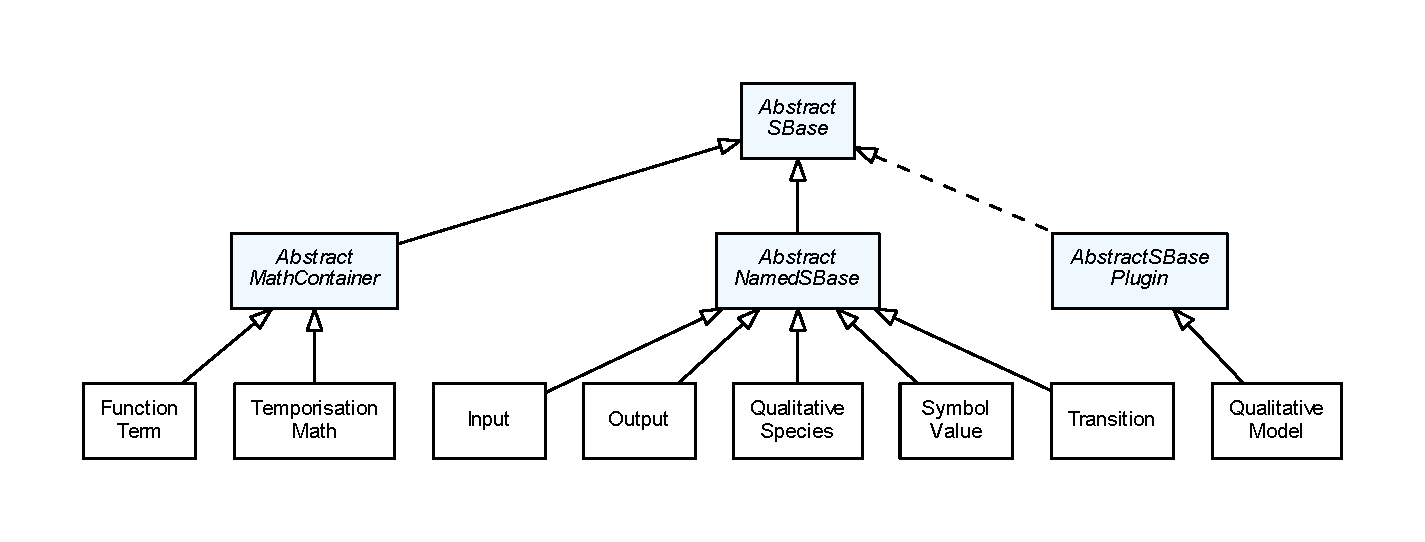
\includegraphics[width=\textwidth]{../../../extensions/qual/doc/img/type_hierarchy.pdf}
 \caption[Class diagram of the qualitative models extension]{Class diagram of the qualitative models extension. Qualitative Models package (\code{qual}, for short) allows species in a model to 
have non-quantitative or non-continuous concentrations \cite{Chaouiya2013}. 
This may manifest as Boolean or discrete values, and is primarily employed in 
modelling gene regulation, signalling pathways, and metabolic networks using 
logical/Boolean networks \cite{shmulevich2002} or Petri nets 
\cite{breitling2008}, which in turn, do not rely on traditional quantitative
coefficients to encode relationships between biochemical entities.}
 \label{fig:qual}
\end{figure}

\begin{figure}[hb]
 \centering
 \vspace*{2ex}
 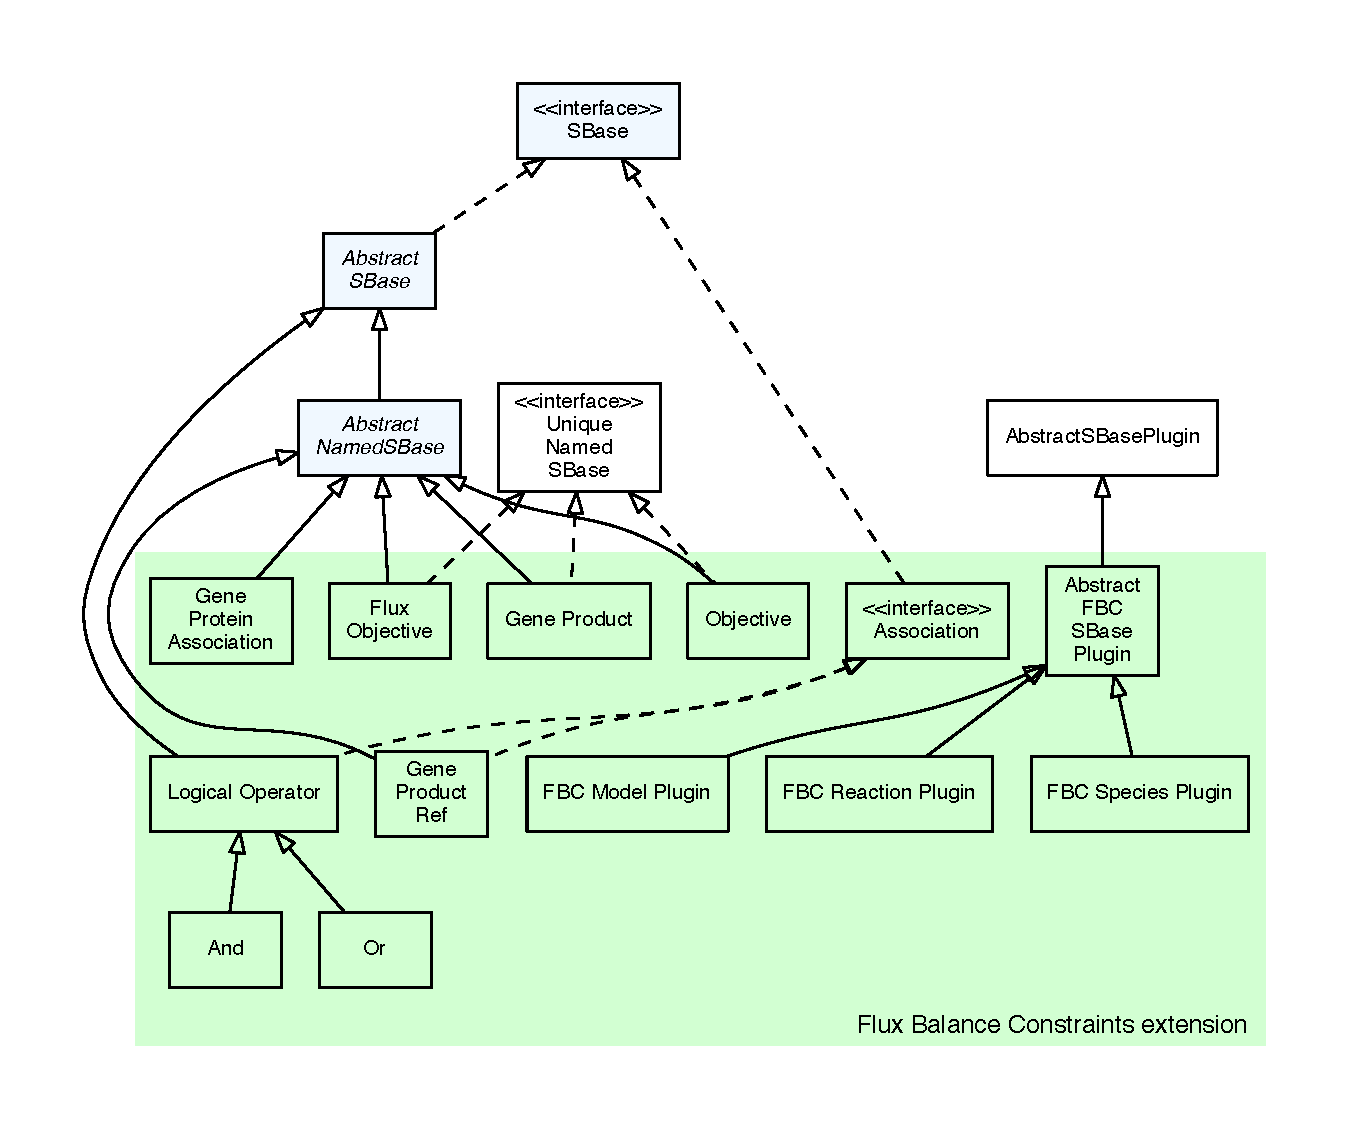
\includegraphics[width=\textwidth]{../../../extensions/fbc/doc/img/type_hierarchy.pdf}
 \caption[Class diagram of the flux balance constraints extension.]{Class diagram of the flux balance constraints extension. Constraints-based modelling \cite{lewis2012} utilizes a class of models in which
the canonical stoichiometric relations between reactions and metabolites are specified
as constraints for convex analysis and mathematical optimization. Although species,
reactions, and stoichiometry can be encoded using the SBML L3V1,
Flux Balance Constraints (\code{fbc}, \cite{olivier2013}) enable a constraints
based perspective. For example, the constraints based approach called
Flux Balance Analysis (FBA) often aims to find the maximum growth rate of the
cell given a set of uptake possibilities and the ratio of molecules needed
for cell growth. The mathematical formulation for this optimization problem
has variables of reaction fluxes and constraints of mass balances around the
metabolites and bounds on the variable reaction fluxes. Because this formulation is
underdetermined, an objective, usually one that maximizes a biomass function which
corresponds to growth rate, is supplied which optimizes the reaction fluxes. Therefore,
the \code{fbc} package extends the SBML Level 3 core to specifically encode for bounds on
fluxes, constraints, and objective functions, which facilitates a fluid interface to
existing constraints-based modelling software and optimization solvers.}
 \label{fig:fbc}
\end{figure}

\begin{figure}[hb]
 \centering
 \vspace*{2ex}
 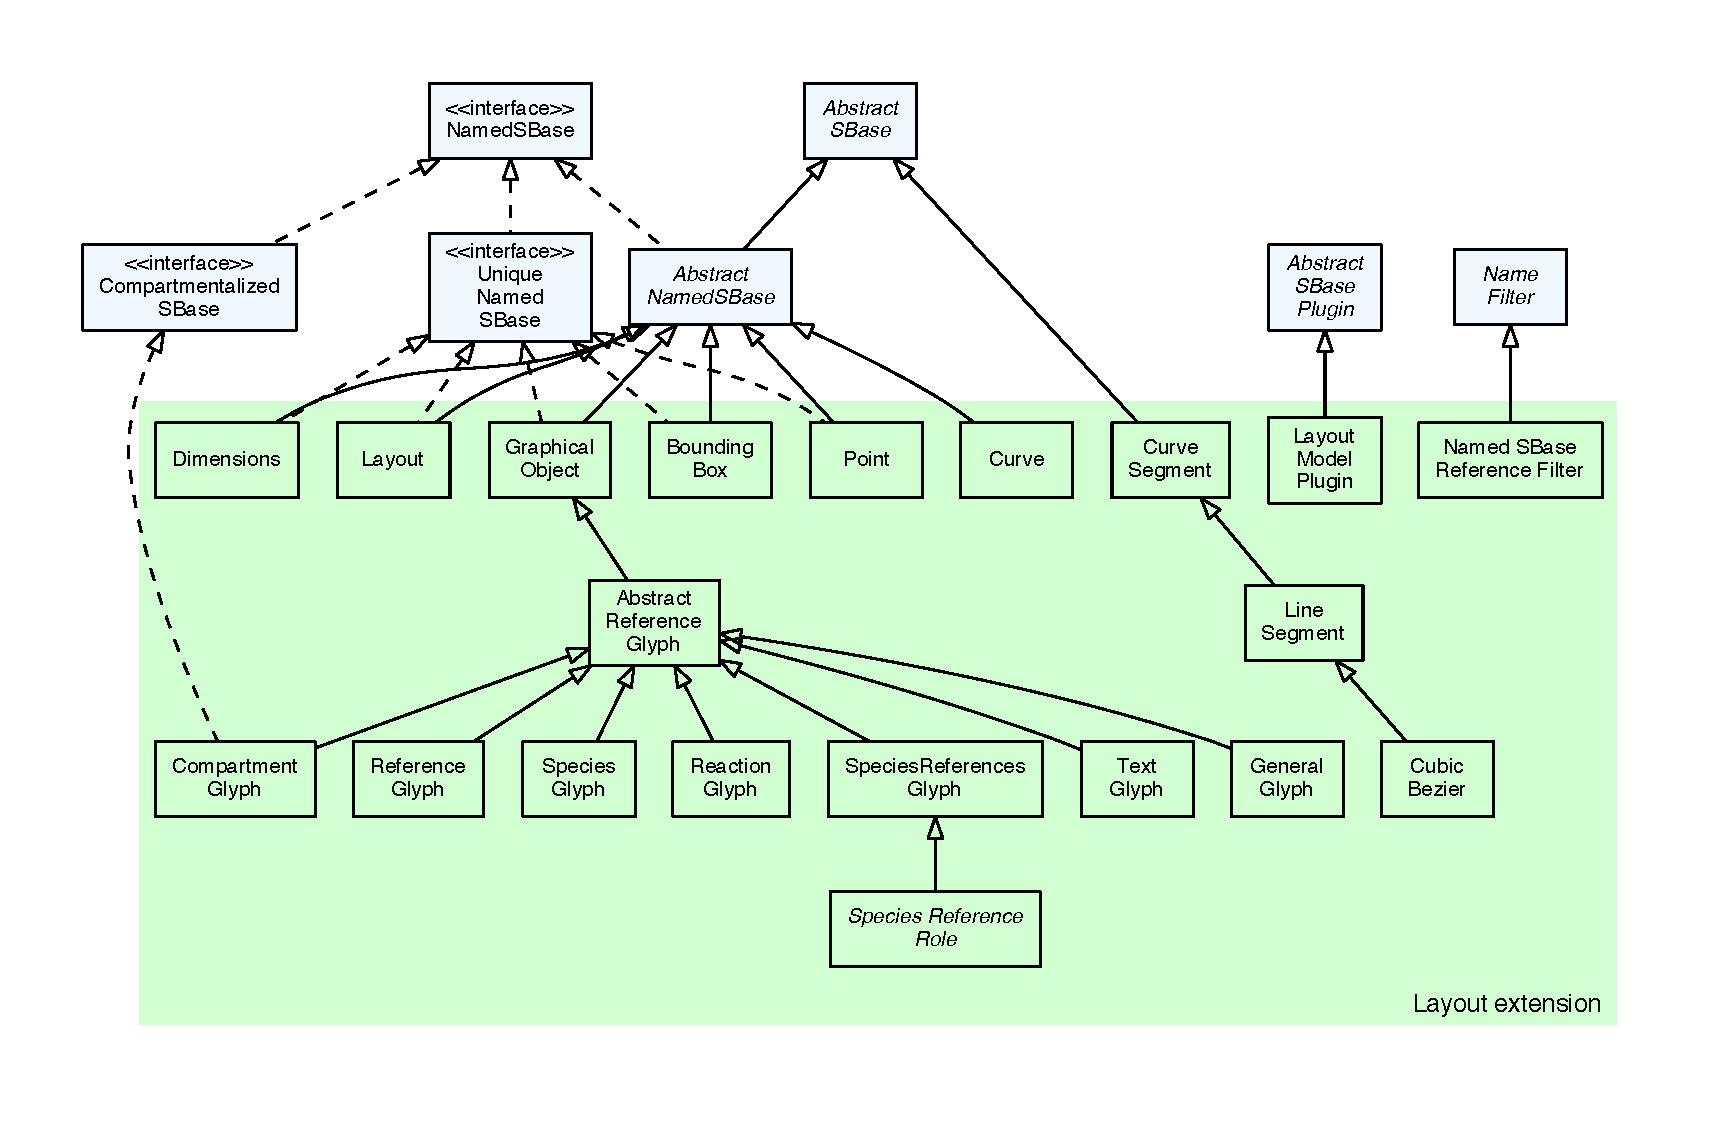
\includegraphics[width=\textwidth]{../../../extensions/layout/doc/img/type_hierarchy.pdf}
 \caption[Class diagram of the layout extension]{Class diagram of the layout extension. SBML encodes a core set of components (species, reactions) that make up
biochemical networks. The \code{layout} extension supports specifying graphical
information for these components. The structure for this extension mirrors 
the SBML Level 3 core hierarchy by introducing graphical object (\code{glyph})
counterparts to reactions and species. Different \code{glyph} types can optionally correspond
to elements in standard SBML, and there can be many \code{glyphs} for one element.
In addition, \code{layout} elements of non-standard model components can be specified
using the generic \code{GraphicalObject} class. Although this extension is powerful
enough to encode the position of all biochemically related graph components,
it should be noted that the scope of this package does not include rendering
of these components. This functionality is provided by the \code{Render} package.
Ultimately, the \code{layout} extension provides a common language that biochemical
graph editors and viewers can utilize to couple a model to a graph layout.}
 \label{fig:layout}
\end{figure}

\begin{figure}[hb]
 \centering
 \vspace*{2ex}
 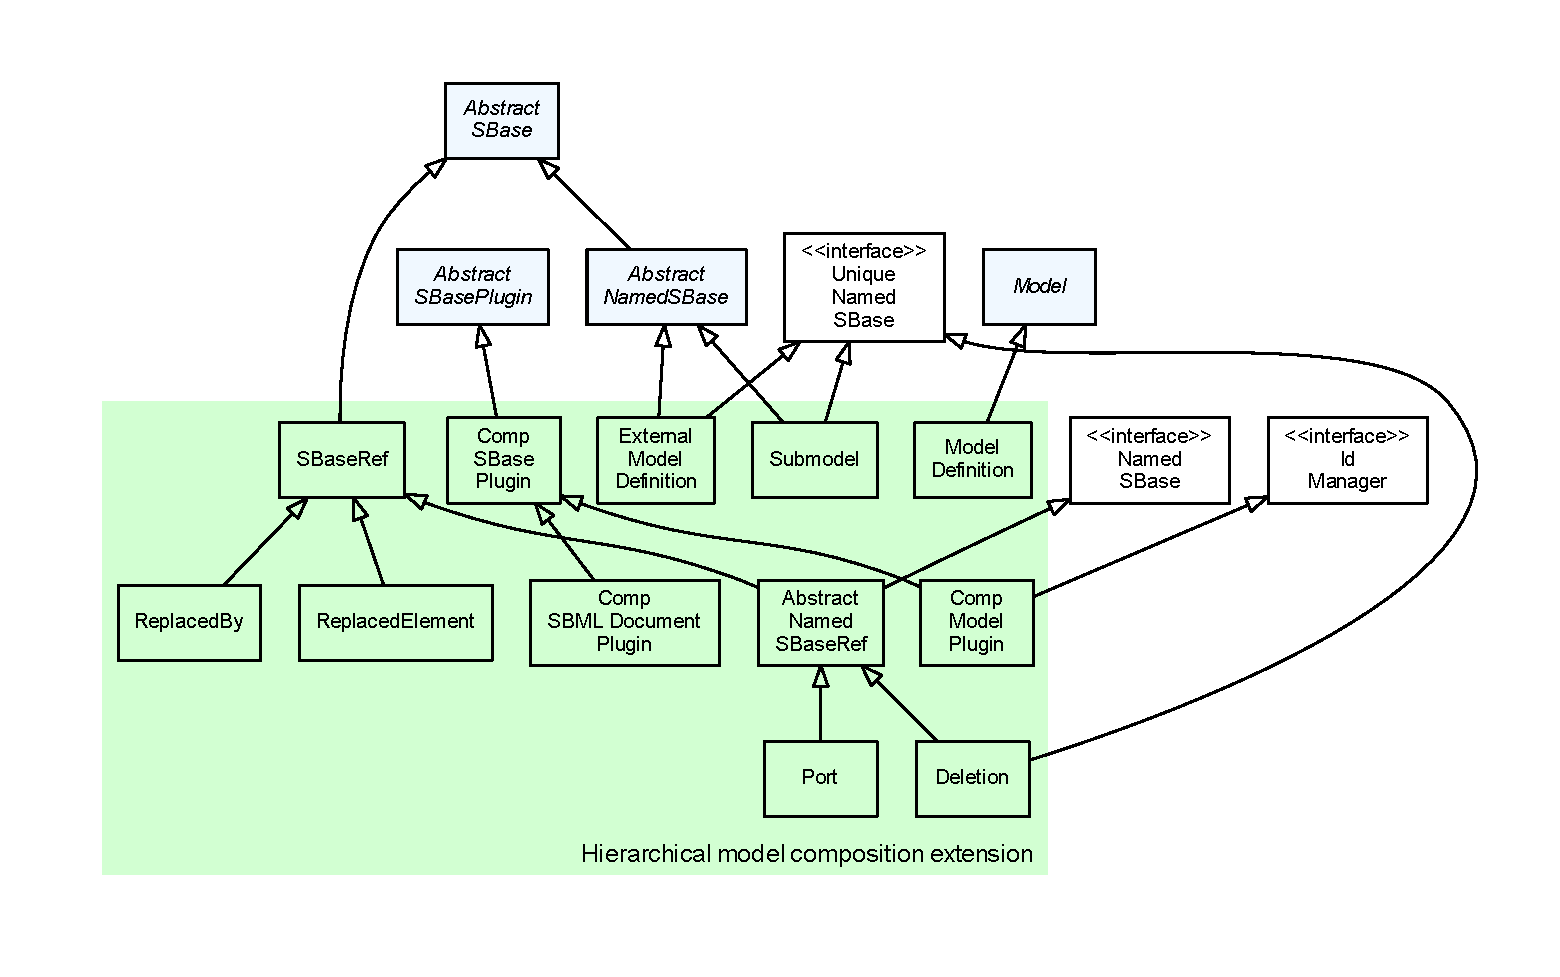
\includegraphics[width=\textwidth]{../../../extensions/comp/doc/img/type_hierarchy.pdf}
 \caption[Class diagram of the hierarchical model composition extension]{Class diagram of the hierarchical model composition extension. As the amount of information for biochemical networks increases, models tend to
increase in complexity as well. The Hierarchical Model Composition extension (\code{comp}; \cite{smith2010})
attempts to contextualize this complexity by providing a generic framework to encode
models as hierarchical entities in an SBML document. This functionality also allows
for storing multiple instances of a model within an enclosing model or document, which
can be used to build libraries of models within a document or to independently manage
different parts of a large model. Classes allow modellers to access elements within
sub-models and interface with other sub-models, and \code{comp} provides a standardized approach
to define sub-model differences with respect to parent or reference models. Overall, \code{comp}
is a powerful extension to the SBML Level 3 core that gives modellers and programmers
options to standardize the encoding of complex, modular modelling frameworks. 
}
 \label{fig:comp}
\end{figure}

\begin{figure}[hb]
 \centering
 \vspace*{2ex}
 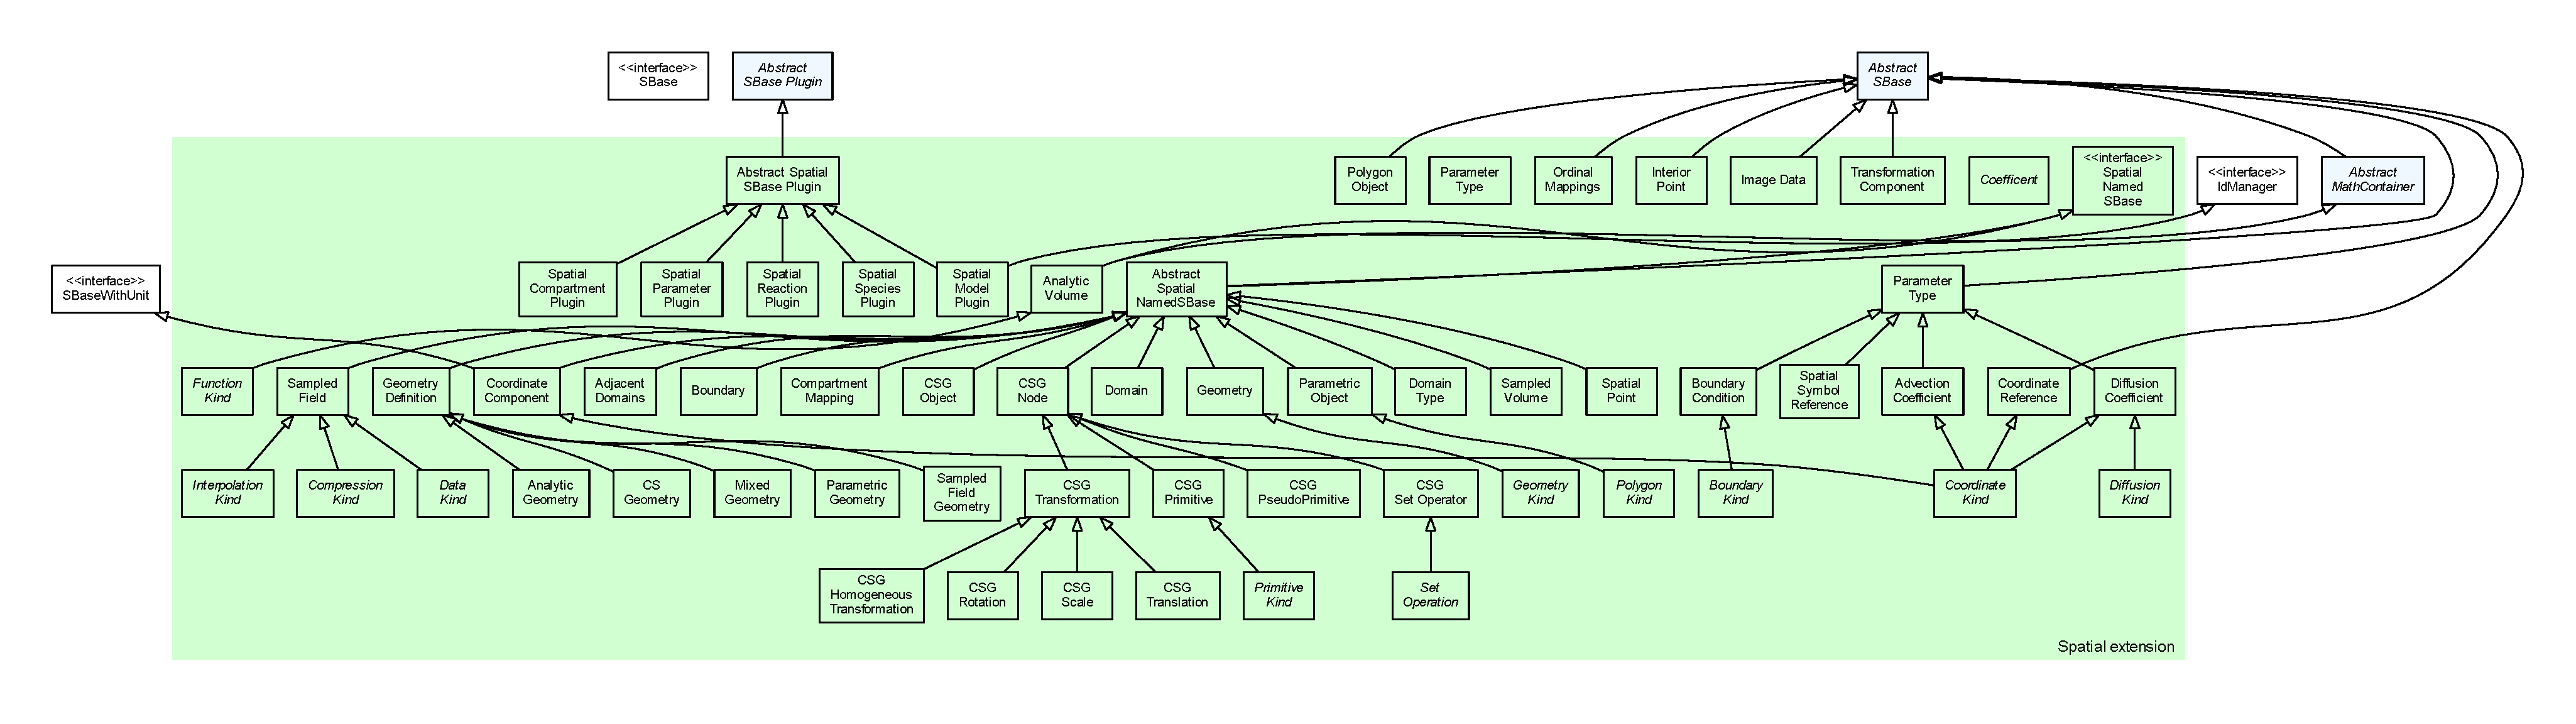
\includegraphics[width=\textwidth]{../../../extensions/spatial/doc/img/type_hierarchy.pdf}
 \caption[Class diagram of the spatial processes extension]{Class diagram of the spatial processes extension. The Spatial Processes extension (\code{spatial}, \cite{Schaff2014})
provides the ability to the SBML Level 3 core to specify subcellular,
geometric locations for components in biochemical
models. Although subcellular locations can be abstractly represented via
compartments in the SBML core specifications, \code{spatial} enables the encoding of
a cellular coordinate system which can describe non-uniform molecular distributions,
diffusive transport, and spatially localized reactions. The \code{Geometry} class holds
the spatial information and the extended \code{Species}, \code{Reaction}, \code{Compartment}, and
\code{Parameter} objects have mappings to the \code{spatial} objects that hold information on
molecular transport coefficients, geometric domains, and coordinates. \code{Spatial} is
therefore able to store the geometric information commonly used in spatial modelling
tools for the biochemical entities from standard SBML.}
 \label{fig:spatial}
\end{figure}

\begin{figure}[hb]
 \centering
 \vspace*{2ex}
 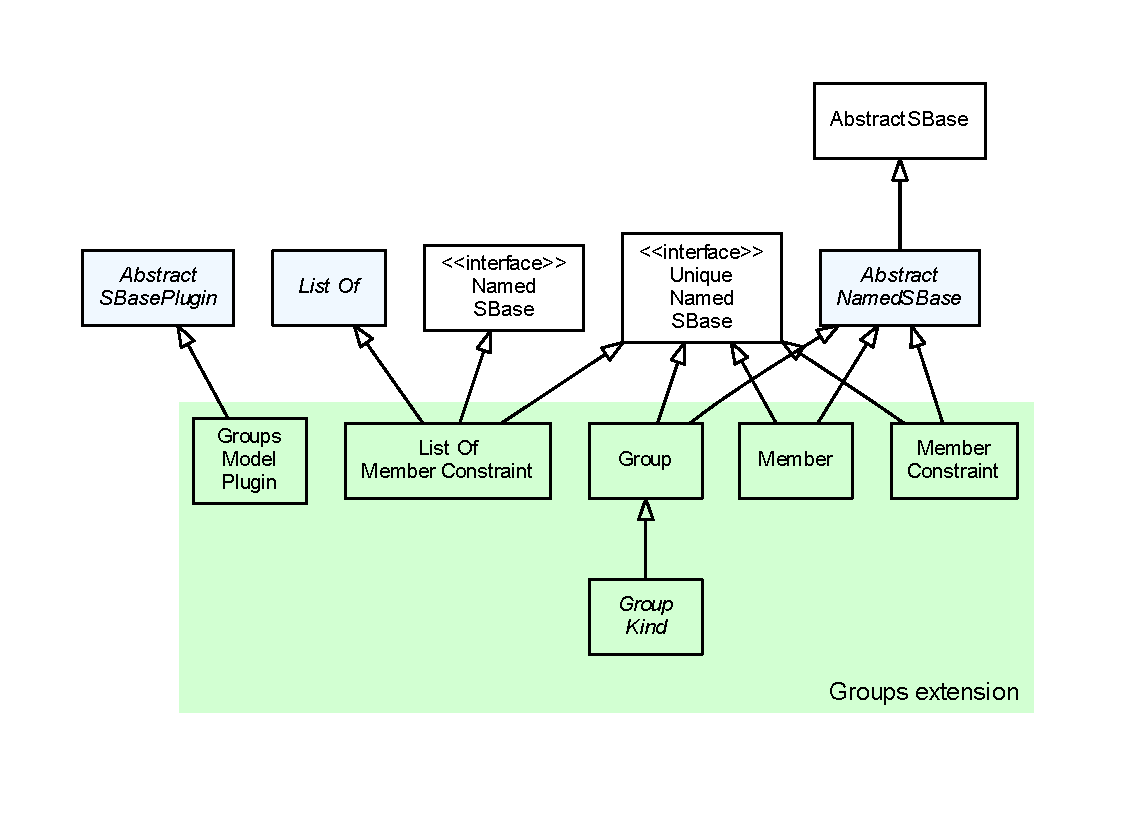
\includegraphics[width=\textwidth]{../../../extensions/groups/doc/img/type_hierarchy.pdf}
 \caption[Class diagram of the groups extension]{Class diagram of the groups extension. \code{Groups} is a simple extension that links together elements in an SBML model. Coupling
\code{groups} information with annotation and SBO terms \cite{Courtot2011a} 
contextualizes these sets of objects for properly conveying roles of groups 
for other programmers and modellers.}
 \label{fig:groups}
\end{figure}


\begin{figure}[hb]
 \centering
 \vspace*{2ex}
 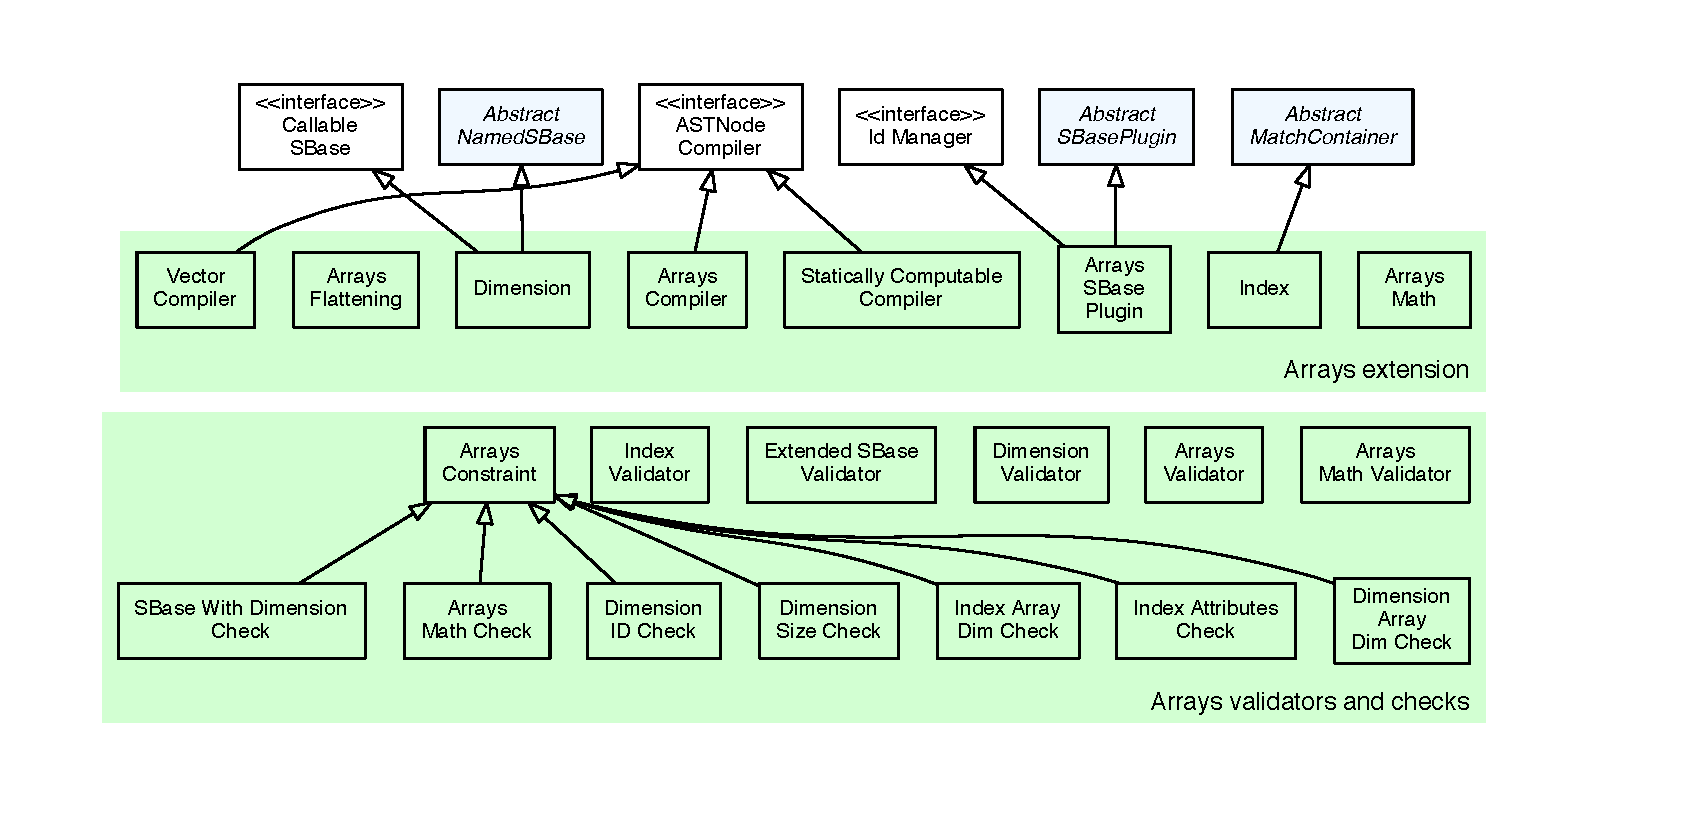
\includegraphics[width=\textwidth]{../../../extensions/arrays/doc/img/type_hierarchy.pdf}
 \caption[Class diagram of the arrays extension]{Class diagram of the arrays extension. Arrays (\code{arrays}, \cite{Watanabe2013}) extends SBML variables to include arrays of values,
thereby representing repeated or regular model structures more efficiently.
\code{Arrays} provides the ability to access sets of values with indices instead of explicit
declaration and creation of sub-data objects.}
 \label{fig:arrays}
\end{figure}


\begin{figure}[hb]
 \centering
 \vspace*{2ex}
 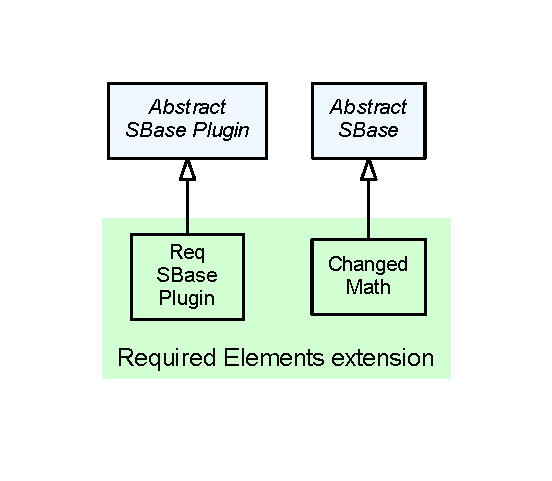
\includegraphics[width=.5\textwidth]{../../../extensions/req/doc/img/type_hierarchy.pdf}
 \caption[Class diagram of the required elements extension]{Class diagram of the required elements extension. Required Elements (\code{req}, \cite{Smith2013}) allows a model to indicate which
components have had their mathematical meanings changed by (e.g.) the use of
another SBML package.}
 \label{fig:arrays}
\end{figure}


\begin{figure}[hb]
 \centering
 \vspace*{2ex}
 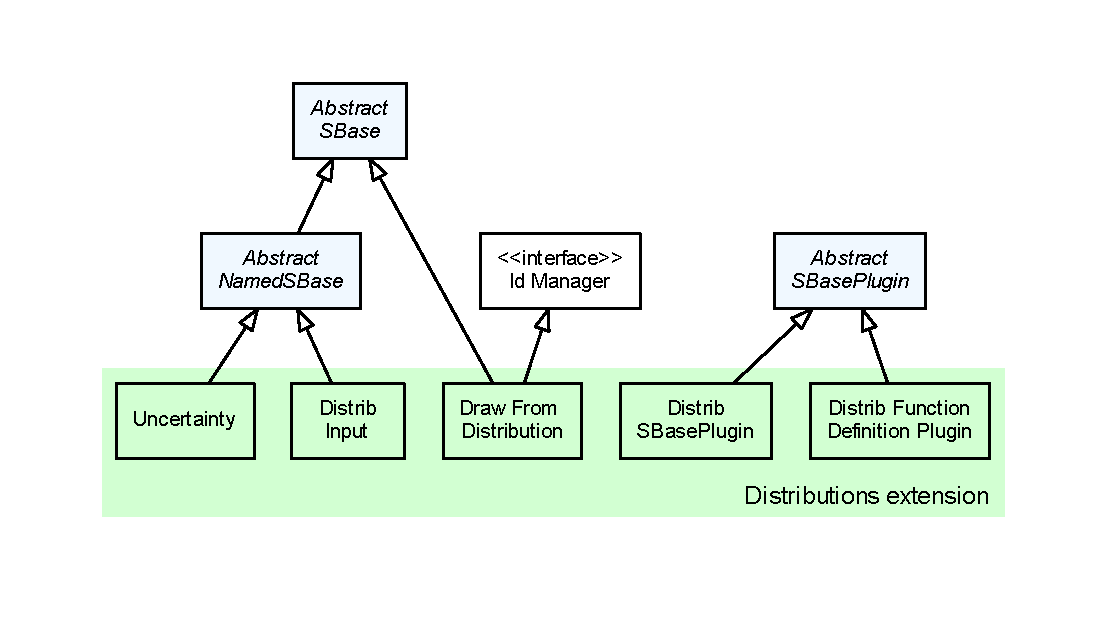
\includegraphics[width=\textwidth]{../../../extensions/distrib/doc/img/type_hierarchy.pdf}
 \caption[Class diagram of the distributions extension.]{ Class diagram of the distributions extension. Distributions 
 (\code{distrib}, \cite{Moodie2013}) encodes statistical distributions and their sampling.}
 \label{fig:distrib}
\end{figure}

\begin{figure}[hb]
 \centering
 \vspace*{2ex}
 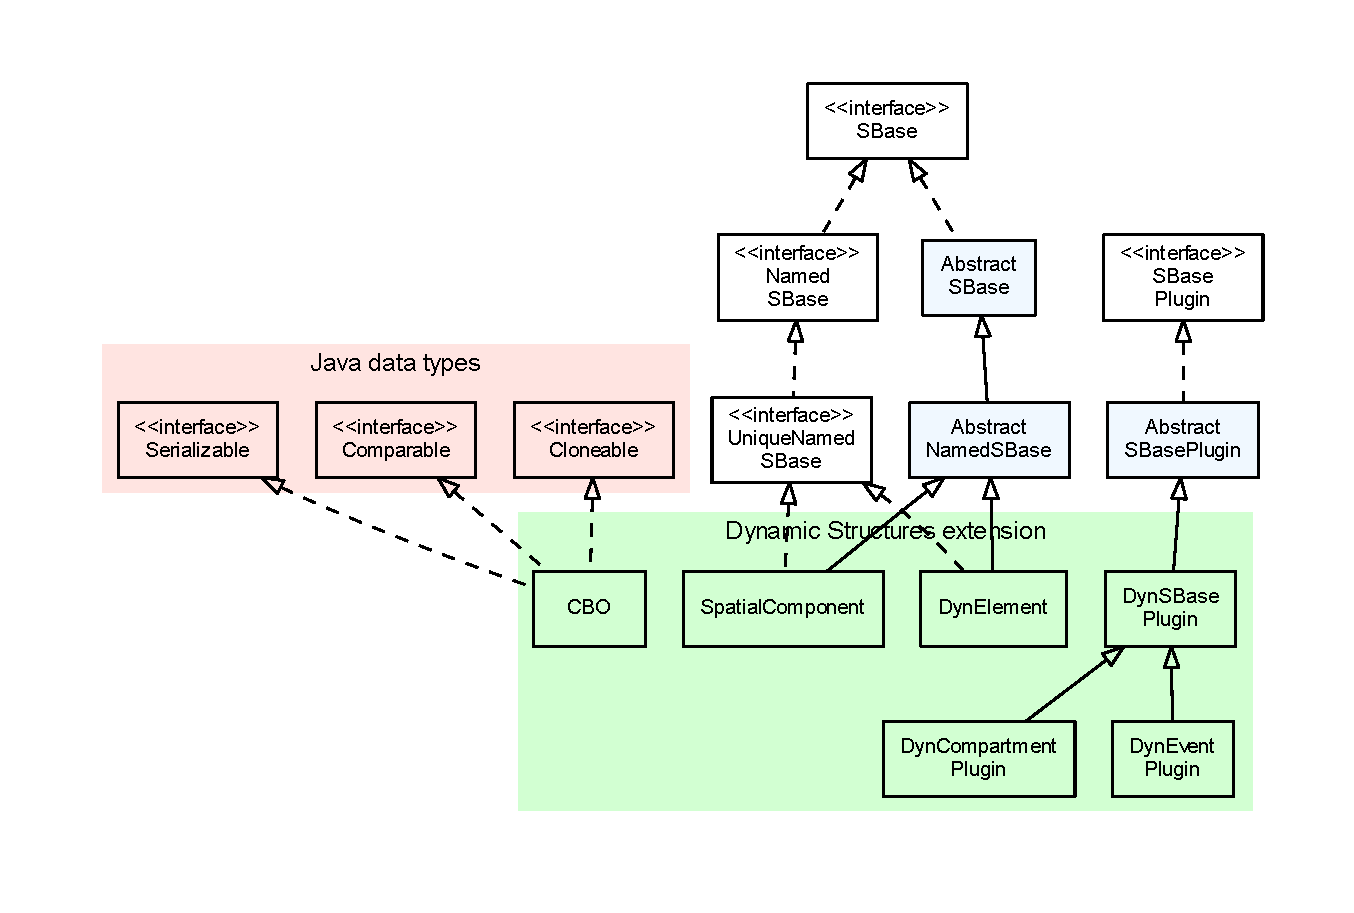
\includegraphics[width=\textwidth]{../../../extensions/dyn/doc/img/type_hierarchy.pdf}
 \caption[Class diagram of the dynamic structures extension]{Class diagram of the dynamic structures extension. Dynamic Structures (\code{dyn}, \cite{Gomez2014}), supports the definition of dynamical behaviors for model entities.
}
 \label{fig:dyn}
\end{figure}


\begin{figure}[hb]
 \centering
 \vspace*{2ex}
 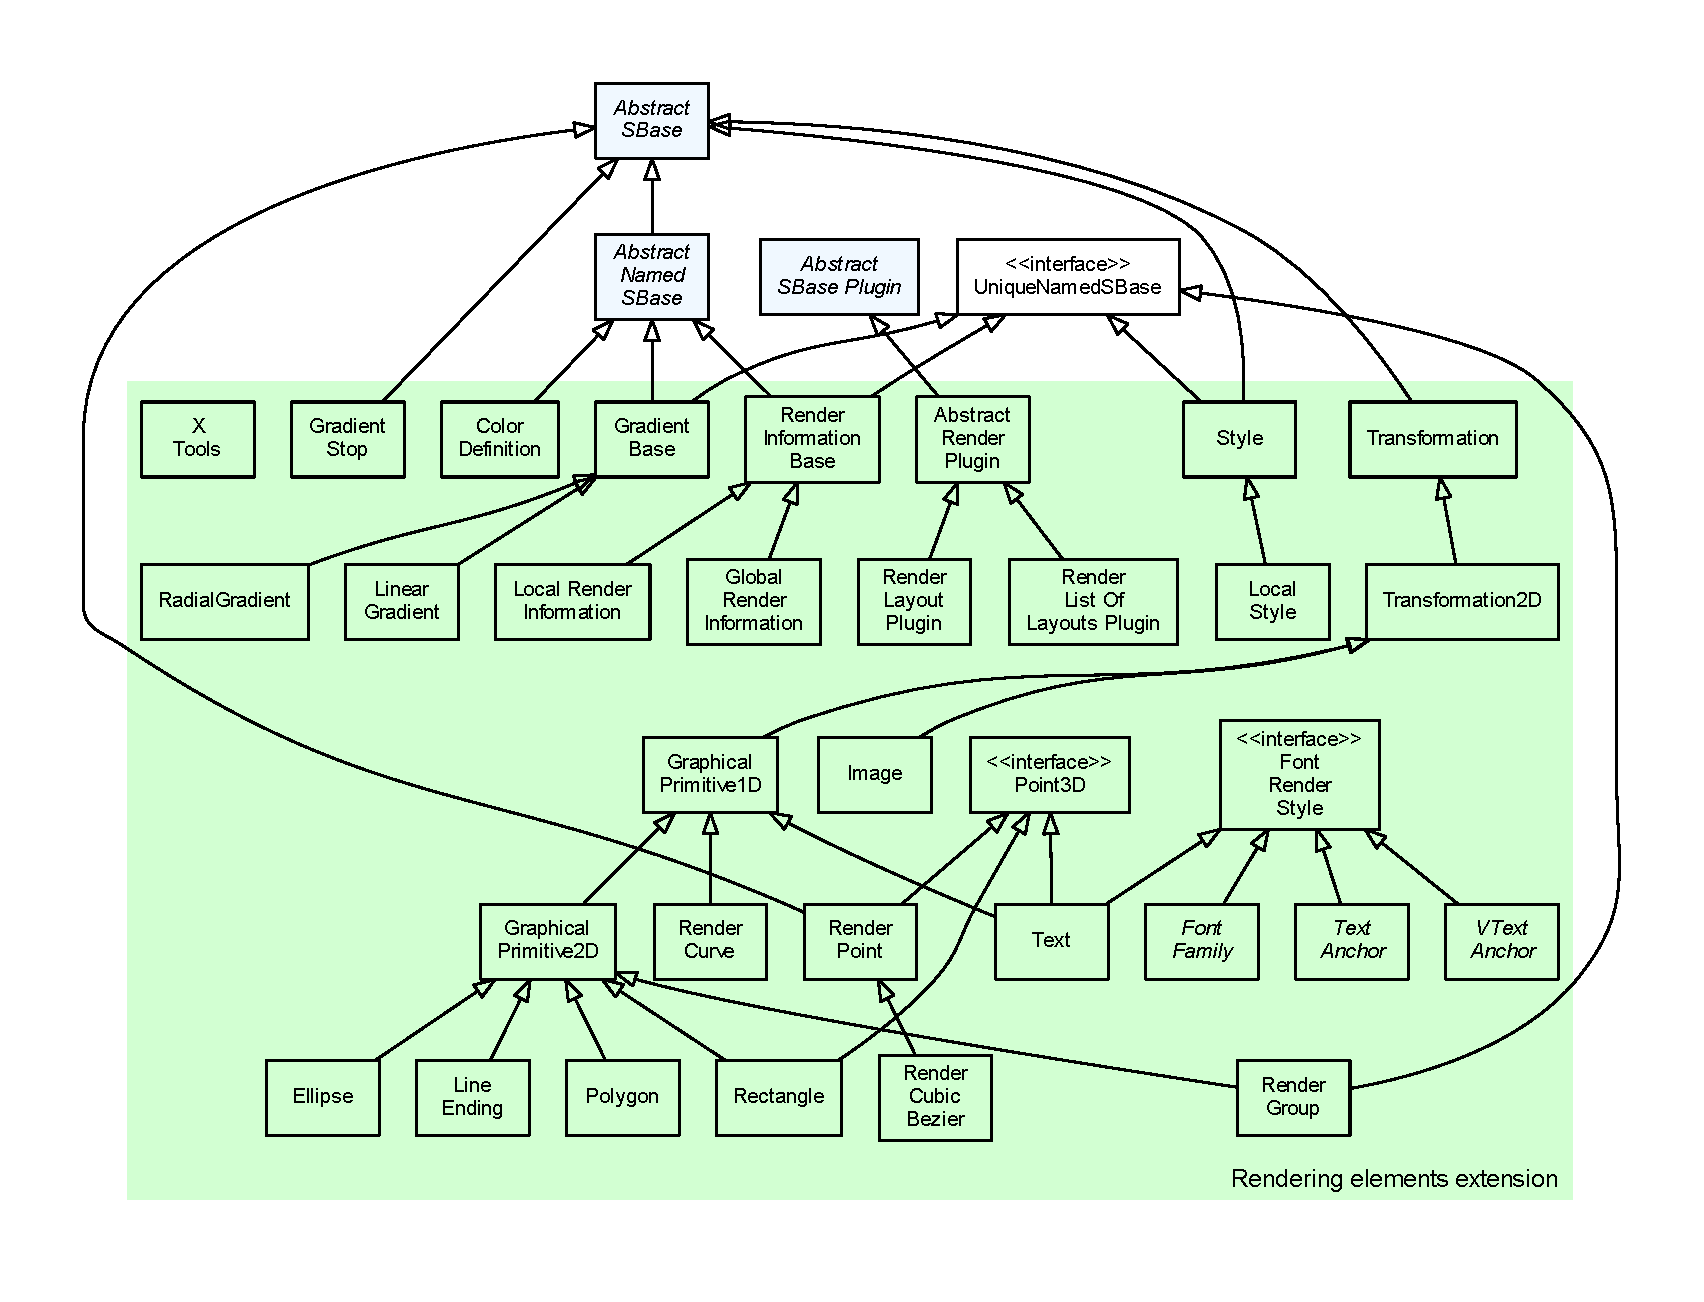
\includegraphics[width=\textwidth]{../../../extensions/render/doc/img/type_hierarchy.pdf}
 \caption[Class diagram of the rendering extension.]{Class diagram of the rendering extension. Rendering (\code{render}, \cite{gauges2006}) couples with \cite{Layout} to provide symbol and style information for network diagrams.}
 \label{fig:render}
\end{figure}



\chapter{Acknowledgments}
\label{chp:acknowledgements}

% -*- TeX-master: "User_guide"; fill-column: 75 -*-

The development and support of JSBML is a substantial undertaking and many
people have put in time and effort on this project.  The authors especially
thank the following individuals for their many contributions to JSBML:
Meike Aichele, Sebastian Fr\"ohlich, Roland Keller, Sarah Rachel M\"uller
vom Hagen, Alexander Peltzer, and Simon Sch\"afer (in alphabetical order).

The development of JSBML is currently funded by the following
organizations:

\begin{itemize}

\item The National Institute of General Medical Sciences (USA) via grant
number R01~GM070923, 

\item The EMBL European Bioinformatics Institute (Germany and UK), and

\item The Federal Ministry of Education and Research (BMBF, Germany) via grant numbers 0315756 and 0315384C for the \emph{Virtual Liver Network} and the MedSys (Medical Systems Biology) project \emph{Spher4Sys}.

\end{itemize}

Last but not least, JSBML is an open-source project, and we thank others
who have helped in its progress, in the form of comments, bug reports, bug
fixes, and other contributions.

Other interested people are welcome to join the team and to contribute to
the project.  The JSBML Team also explicitely encourages students who would
like to participate in a large software project, to ask for current
JSBML subprojects that are in need of doing.



\appendix

\chapter{Frequently Asked Questions (FAQ)}
\label{chp:faq}

For questions regarding SBML, please see the SBML FAQ at
\url{http://sbml.org/Documents/FAQ}.
\begin{description}
\item[Why does the class \texttt{LocalParameter} not inherit from
\texttt{Parameter}?]
\index{parameter!\texttt{LocalParameter}}
\index{parameter!\texttt{Parameter}}
The reason is the Boolean
\index{Boolean}
attribute \texttt{constant}, which is present in
\index{constant}
\index{parameter!\texttt{constant}}
\texttt{Parameter} and can be set to \texttt{false}. A parameter in the meaning
of SBML is not a constant, it might be some system variable
\index{JSBML!variable@\texttt{Variable}}
and can therefore be the subject of \texttt{Rule}s,
\index{rule}
\texttt{Event}s\index{event!\texttt{Event}}, \texttt{InitialAssignment}s
\index{InitialAssignment@\texttt{InitialAssignment}}
and so on, i.e., all instances of \texttt{Assignment},
\index{JSBML!assignment@\texttt{Assignment}}
whereas a \texttt{LocalParameter} is defined as a constant quantity that never
changes its value during the evaluation of a model\index{model}. It would
therefore only be possible to let \texttt{Parameter} inherit from
\texttt{LocalParameter} but this could lead to a semantic misinterpretation.


\item[Does JSBML depend on SWING or any particular graphical user interface
implementation?]
Although all classes in JSBML implement the \texttt{TreeNode} interface, which
is located in the package \texttt{javax.swing.tree}, all classes in JSBML are
entirely independent from any graphical user interface, such as the SWING
implementation. When loading the \texttt{TreeNode} interface, no other class
from SWING will be initialized or loaded; hence JSBML can also be used on
computers that do not provide any graphical system without the necessity of
catching a \texttt{HeadlessException}. The \texttt{TreeNode} interface only
defines methods and properties that all recursive tree data structures have to
implement anyway. Letting JSBML classes extend this interface makes JSBML
compatible with many other Java classes and methods that make use of the
standard \texttt{TreeNode} interface, hence ensuring a high compatibility with
other Java libraries. Since the SWING package belongs to the standard
Java\texttrademark{} distribution, it is ensured that the \texttt{TreeNode}
interface can always be localized by the Java Virtual Machine,
independent from the specific hardware or system.

\item[Does the usuage of the the \texttt{java.beens} package for the
\texttt{TreeNodeChangeListener} lead to an incompatibility with light-weight
Java installations?]
With the \texttt{java.beens} package being part of the standard Java
distribution, such an incompatibility will not occur. Extending existing
standard Java classes leads to a higher compatibility with other libraries and
should therefore be the preferred way to go in the development of JSBML.
\end{description}



\chapter{Open tasks in JSBML development}
\label{chp:open-tasks}

\begin{itemize}
\item JSBML does not yet provide a complete validator for SBML.
\item The support for SBML Level 3\index{SBML!Level~3} should be completed, particularly extension packages.\index{SBML!extension packages}
\item The \texttt{toSBML()}\index{SBase@\texttt{SBase}!\texttt{toSBML()}}
methods in \texttt{SBase} are still missing.
\item Constructors and methods with namespaces are not yet provided.
\item The libSBML compatibility module\index{libSBML!compatibility module} need
to be implemented.
\end{itemize}



\clearpage

\thispagestyle{plain}
\pagestyle{plain}
\bibliography{../common/tex/literature}

% Index
\setindexprenote{\vspace*{0.1ex}}
\printindex

\end{document}



% -----------------------------------------------------------------------------
% 2012-04-06 <mhucka@caltech.edu> I think these comments are no longer
% relevant, and can be deleted.  They were originally below the abstract above.


% It includes instructions and descriptions of where and how to obtain the JSBML
% library and the JSBML modules.

%Although the libraries JSBML and libSBML, used to work with files and data
%structures defined in SBML (Systems Biology Markup Language), are
%very similar and share a common scope, users should be informed about their
%major differences to help switch more easily from one library to the other. To
%this end, the document at hand gives a brief overview of the main differences
%between the Java\texttrademark{} application programming interfaces (API) of
%both libraries.
%
%In addition, JSBML can be used as a communication layer between the widespread
%application CellDesigner and any application that works with JSBML as its
%internal data structure. An example is given, that demonstrates how to
%convert between CellDesigner's plugin data structures and JSBML objects.
%
%In the same way, it is possible to inter-convert between data structures
%obtained from libSBML and JSBML \textcolor{red}{No need to mention the
%specific versions in the abstract, I think}. We provides an example of how to
%read SBML files with libSBML, turn them into JSBML data structures, manipulate
% them and turn them back to libSBML for writing.
%
%Furthermore, JSBML will provides a compatibility module, whose member classes
%show an identical API as defined in libSBML. In this way, the
%compatibility module will facilitate a switch from libSBML to JSBML and vice
%versa by simply exchanging the included JAR file in the project.
%
%\textcolor{red}{This document gives an example for the usage of the
%compatibility module.}
% Not sure we need to mention in the abstract that we gives examples code for
% each point and anyway, there is not example at the moment for this module.

% I removed the line return for the \index to try to remove the extra spaces
% that were added.
